% Options for packages loaded elsewhere
\PassOptionsToPackage{unicode}{hyperref}
\PassOptionsToPackage{hyphens}{url}
%
\documentclass[
  9pt,
]{book}
\usepackage{amsmath,amssymb}
\usepackage[]{mathpazo}
\usepackage{ifxetex,ifluatex}
\ifnum 0\ifxetex 1\fi\ifluatex 1\fi=0 % if pdftex
  \usepackage[T1]{fontenc}
  \usepackage[utf8]{inputenc}
  \usepackage{textcomp} % provide euro and other symbols
\else % if luatex or xetex
  \usepackage{unicode-math}
  \defaultfontfeatures{Scale=MatchLowercase}
  \defaultfontfeatures[\rmfamily]{Ligatures=TeX,Scale=1}
\fi
% Use upquote if available, for straight quotes in verbatim environments
\IfFileExists{upquote.sty}{\usepackage{upquote}}{}
\IfFileExists{microtype.sty}{% use microtype if available
  \usepackage[]{microtype}
  \UseMicrotypeSet[protrusion]{basicmath} % disable protrusion for tt fonts
}{}
\makeatletter
\@ifundefined{KOMAClassName}{% if non-KOMA class
  \IfFileExists{parskip.sty}{%
    \usepackage{parskip}
  }{% else
    \setlength{\parindent}{0pt}
    \setlength{\parskip}{6pt plus 2pt minus 1pt}}
}{% if KOMA class
  \KOMAoptions{parskip=half}}
\makeatother
\usepackage{xcolor}
\IfFileExists{xurl.sty}{\usepackage{xurl}}{} % add URL line breaks if available
\IfFileExists{bookmark.sty}{\usepackage{bookmark}}{\usepackage{hyperref}}
\hypersetup{
  pdftitle={Supplement to Early childhood linear growth failure in low-and middle-income countries},
  pdfauthor={Jade Benjamin-Chung et al.},
  hidelinks,
  pdfcreator={LaTeX via pandoc}}
\urlstyle{same} % disable monospaced font for URLs
\usepackage{longtable,booktabs,array}
\usepackage{calc} % for calculating minipage widths
% Correct order of tables after \paragraph or \subparagraph
\usepackage{etoolbox}
\makeatletter
\patchcmd\longtable{\par}{\if@noskipsec\mbox{}\fi\par}{}{}
\makeatother
% Allow footnotes in longtable head/foot
\IfFileExists{footnotehyper.sty}{\usepackage{footnotehyper}}{\usepackage{footnote}}
\makesavenoteenv{longtable}
\usepackage{graphicx}
\makeatletter
\def\maxwidth{\ifdim\Gin@nat@width>\linewidth\linewidth\else\Gin@nat@width\fi}
\def\maxheight{\ifdim\Gin@nat@height>\textheight\textheight\else\Gin@nat@height\fi}
\makeatother
% Scale images if necessary, so that they will not overflow the page
% margins by default, and it is still possible to overwrite the defaults
% using explicit options in \includegraphics[width, height, ...]{}
\setkeys{Gin}{width=\maxwidth,height=\maxheight,keepaspectratio}
% Set default figure placement to htbp
\makeatletter
\def\fps@figure{htbp}
\makeatother
\setlength{\emergencystretch}{3em} % prevent overfull lines
\providecommand{\tightlist}{%
  \setlength{\itemsep}{0pt}\setlength{\parskip}{0pt}}
\setcounter{secnumdepth}{5}
\usepackage{booktabs}
\usepackage{amsthm}
\makeatletter
\def\thm@space@setup{%
  \thm@preskip=8pt plus 2pt minus 4pt
  \thm@postskip=\thm@preskip
}
\makeatother
\ifluatex
  \usepackage{selnolig}  % disable illegal ligatures
\fi
\usepackage[]{natbib}
\bibliographystyle{apalike}

\title{Supplement to Early childhood linear growth failure in low-and middle-income countries}
\author{Jade Benjamin-Chung et al.}
\date{2021-07-13}

\begin{document}
\maketitle

{
\setcounter{tocdepth}{1}
\tableofcontents
}
\hypertarget{overview}{%
\chapter{Overview}\label{overview}}

\textbf{Recommended citation:} Benjamin-Chung J, et al.~2020. Early childhood linear growth failure in low-and middle-income countries. \emph{Submitted}. doi.

This site contains supplementary information to the \emph{Early childhood linear growth failure in low-and middle-income countries}.

\hypertarget{QA}{%
\chapter{Quality assurance}\label{QA}}

\raggedright

To check for outliers in length measurements, we plotted the distribution of raw length measurements by age and sex against different percentiles of the World Health Organization child growth standard distribution. The majority of observations fell within 3 standard deviations of the mean of the standard for males and females. There were certain cohorts, such as COHORTs Guatemala, that had a larger proportion of observations outside of 3 standard deviations from the mean. There was a higher variability of length measurements in the PROBIT, ZVITAMBO, and Keneba cohorts.

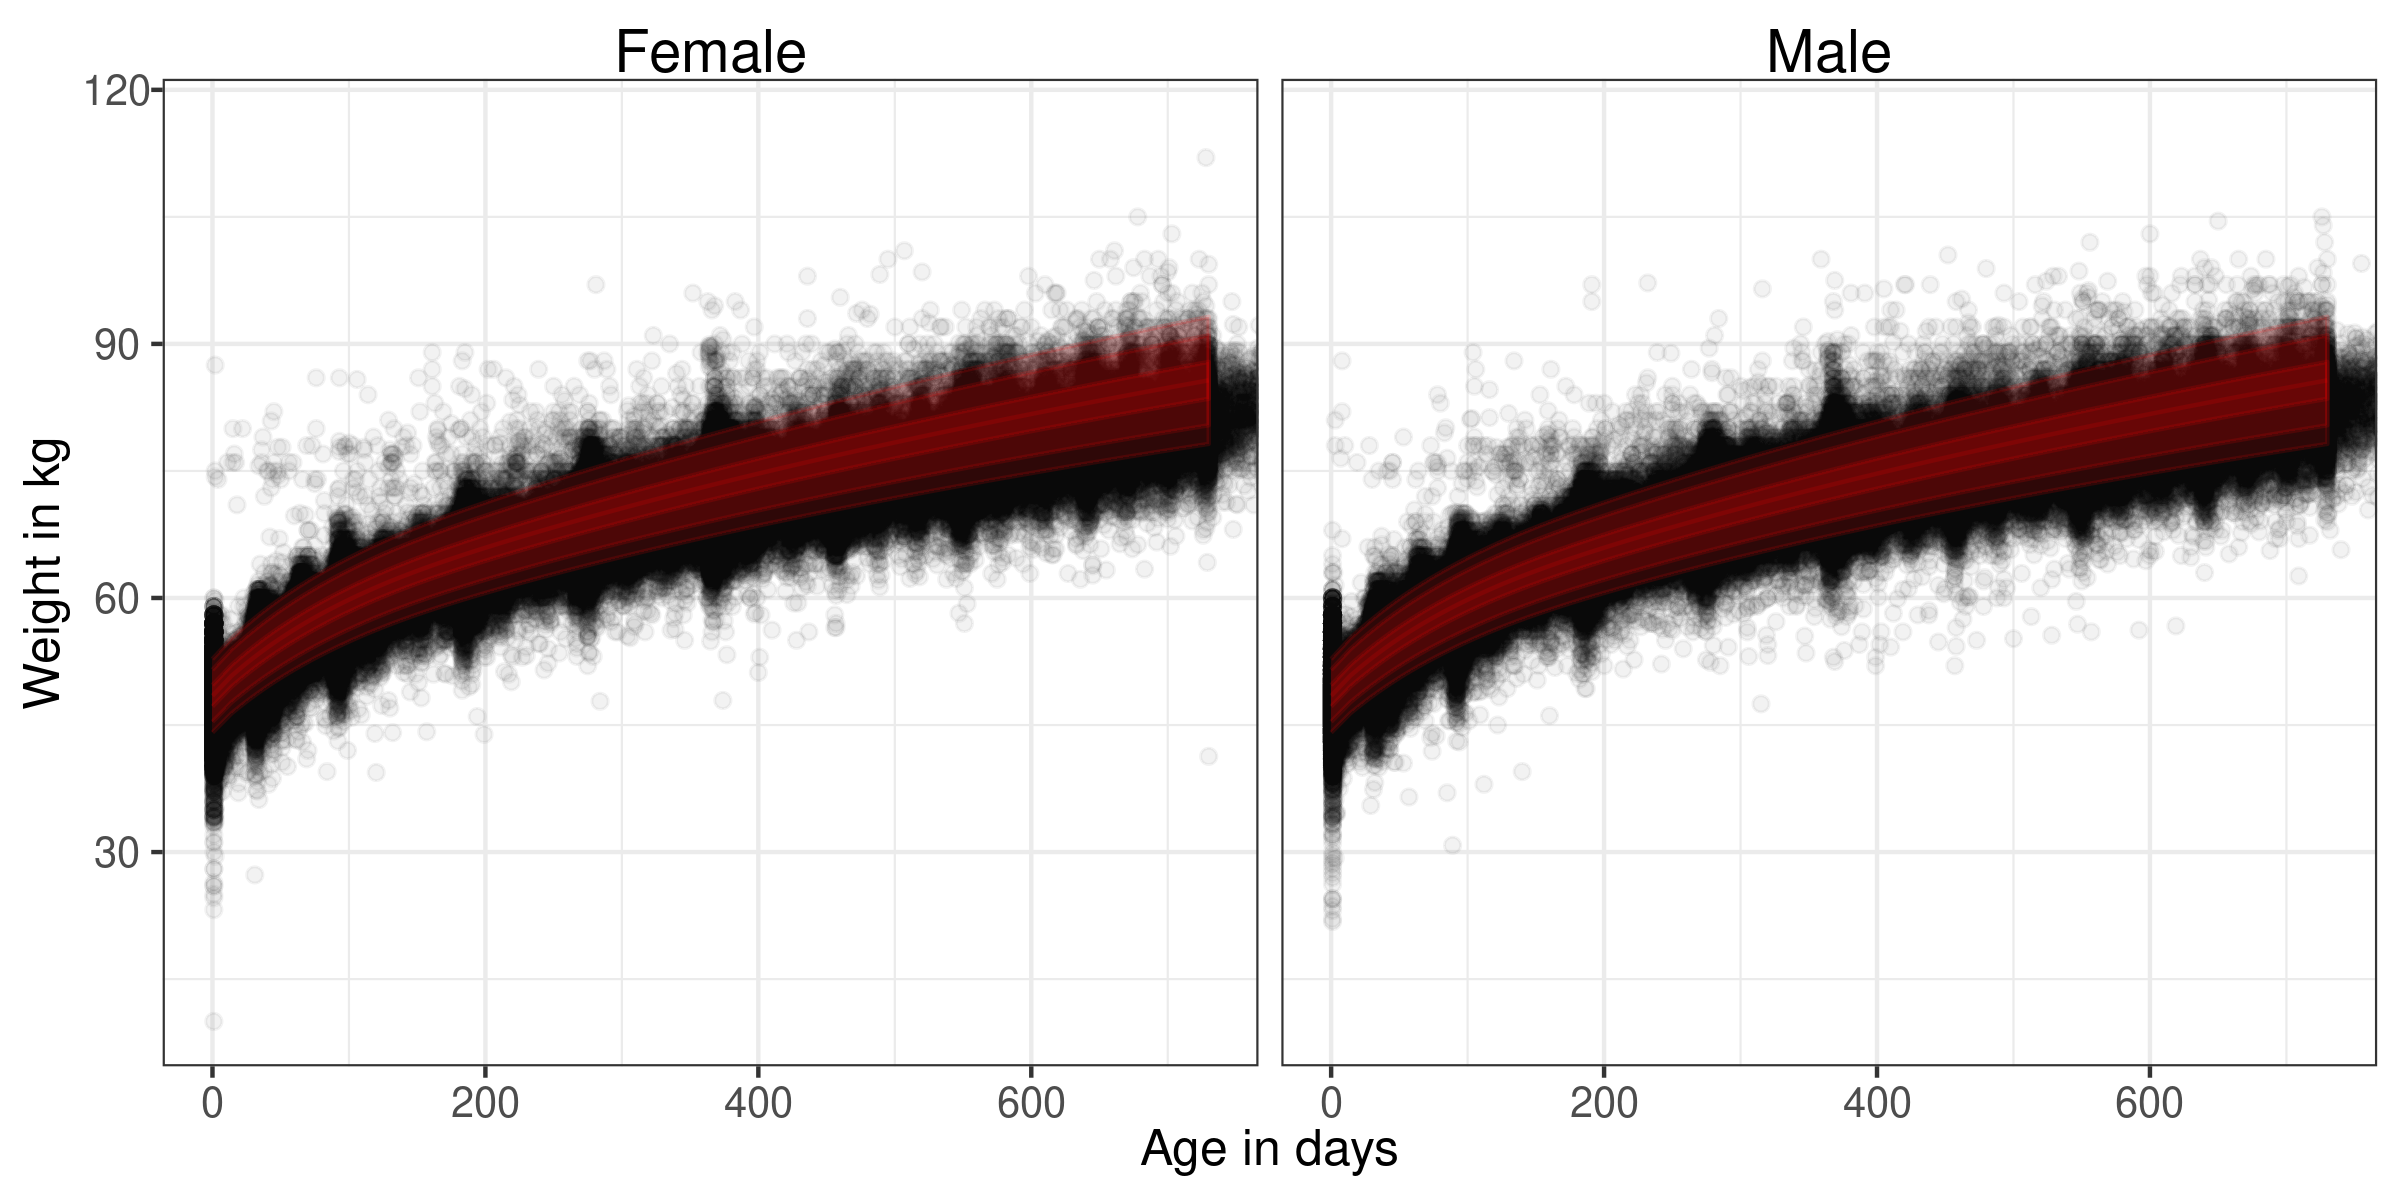
\includegraphics[width=33.33in]{figures//shared/laz_QA}

\includegraphics[width=104.17in]{figures//shared/laz_QA_cohort}

\hypertarget{severe-stunting}{%
\chapter{Severe stunting analyses}\label{severe-stunting}}

\raggedright

Below, we display plots for the age-specific prevalence and cumulative incidence of severe stunting (LAZ \textless{} -3). Overall, the patterns are the same as for stunting (LAZ \textless{} -2), with the peak in prevalence at ages 18-24 months and the highest incidence proportion from 0-3 months.

\hypertarget{age-specific-severe-stunting-prevalence}{%
\section{Age-specific severe stunting prevalence}\label{age-specific-severe-stunting-prevalence}}

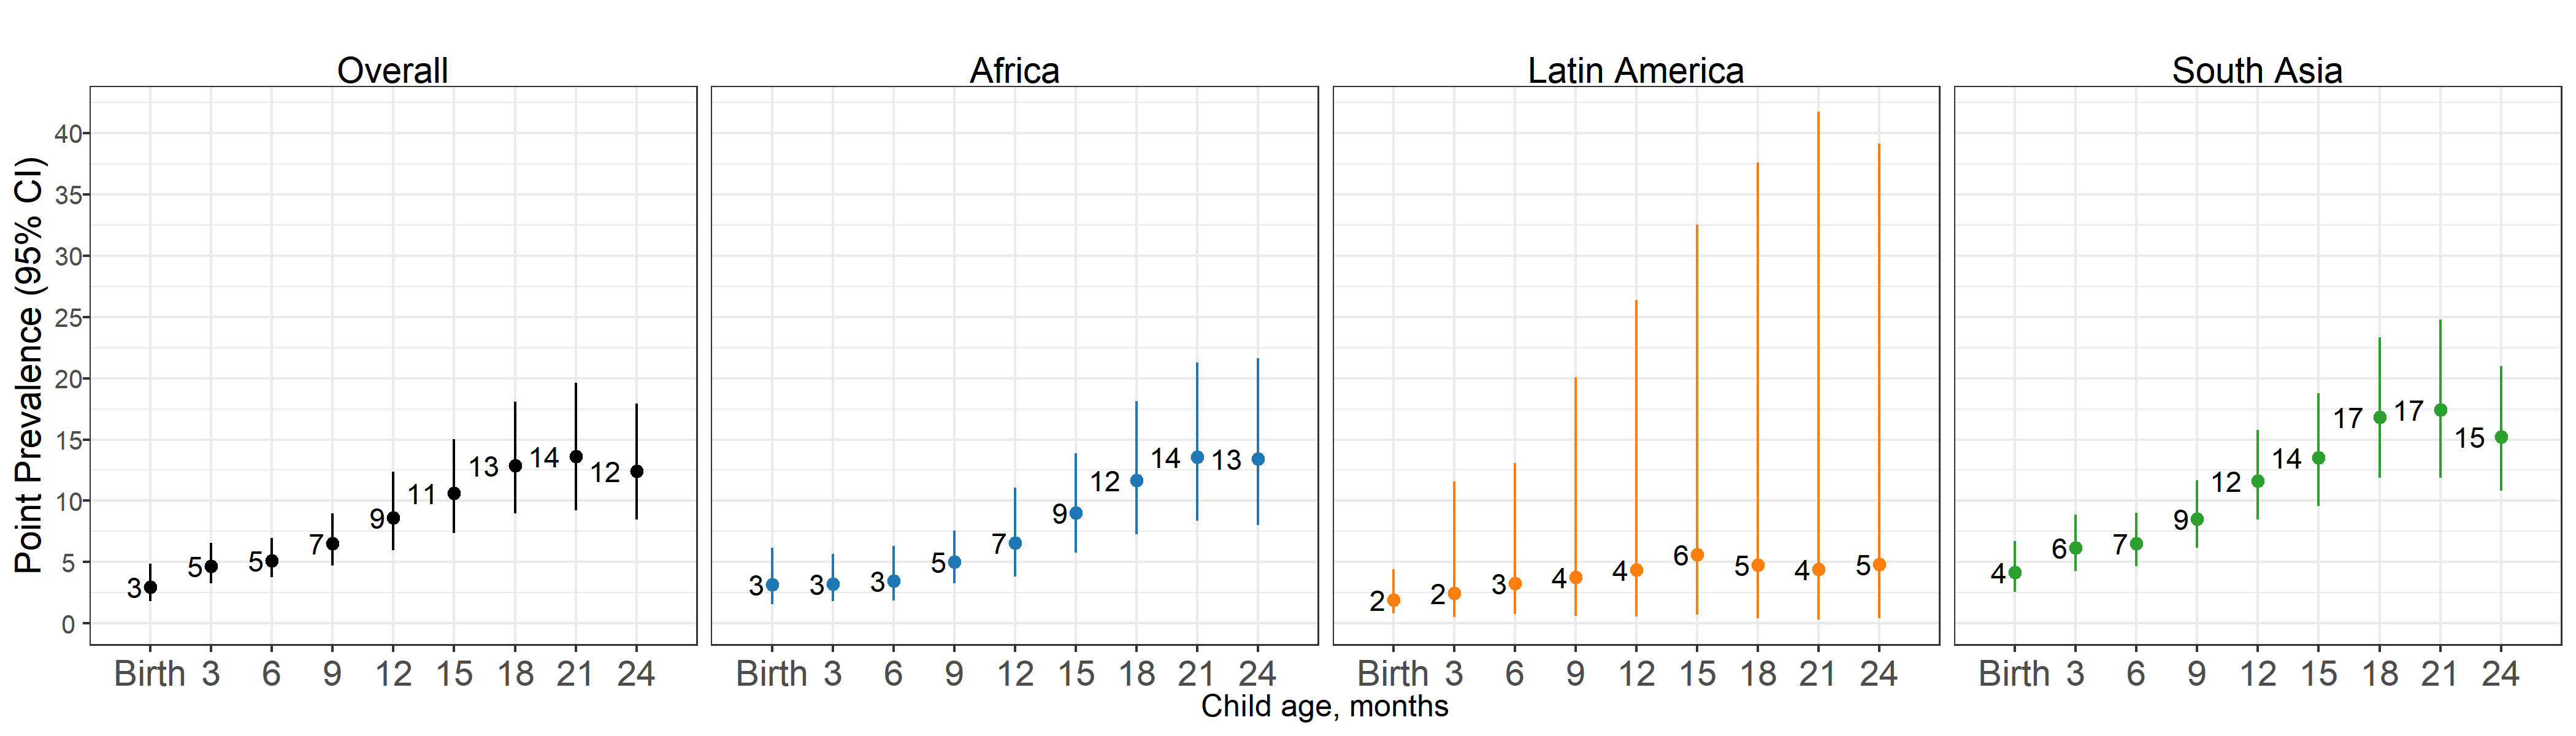
\includegraphics[width=58.33in]{figures//stunting/fig-stunt-3-prev-overall_region--allage-primary}

\hypertarget{age-specific-severe-stunting-incidence}{%
\section{Age-specific severe stunting incidence}\label{age-specific-severe-stunting-incidence}}

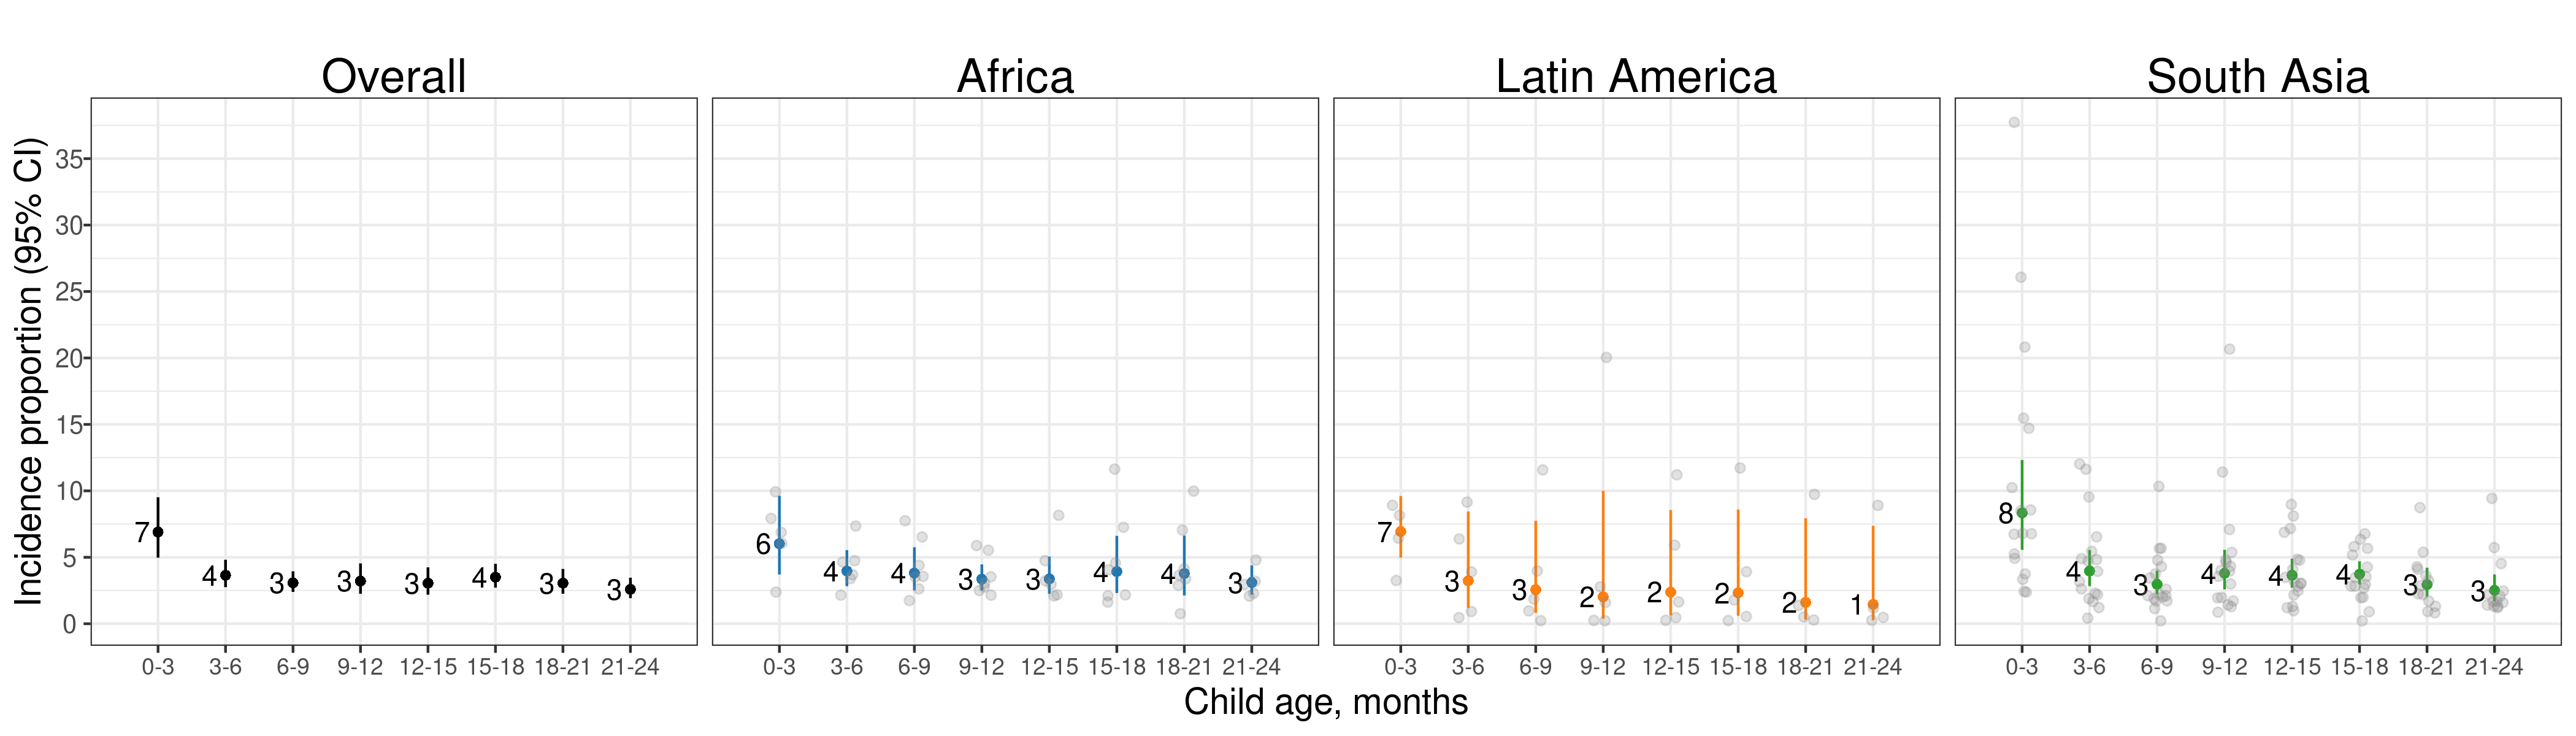
\includegraphics[width=58.33in]{figures//stunting/fig-stunt-3-inc-overall_region--allage-primary}

\hypertarget{secular-trends}{%
\chapter{Assessment of potential secular trends}\label{secular-trends}}

\raggedright

This study included cohorts that measured child growth from 1969 to 2014. To assess potential secular trends, we plotted the mean length-for-age Z-score (LAZ) over time. The plot below shows the individual observations from included studies over this range of years. Curves were fit to the data using generalized additive models, with the solid line fit through the median LAZ by birth year, and the dashed lines mark the 1st and 3rd quartiles. There does not appear to be a secular trend in LAZ.

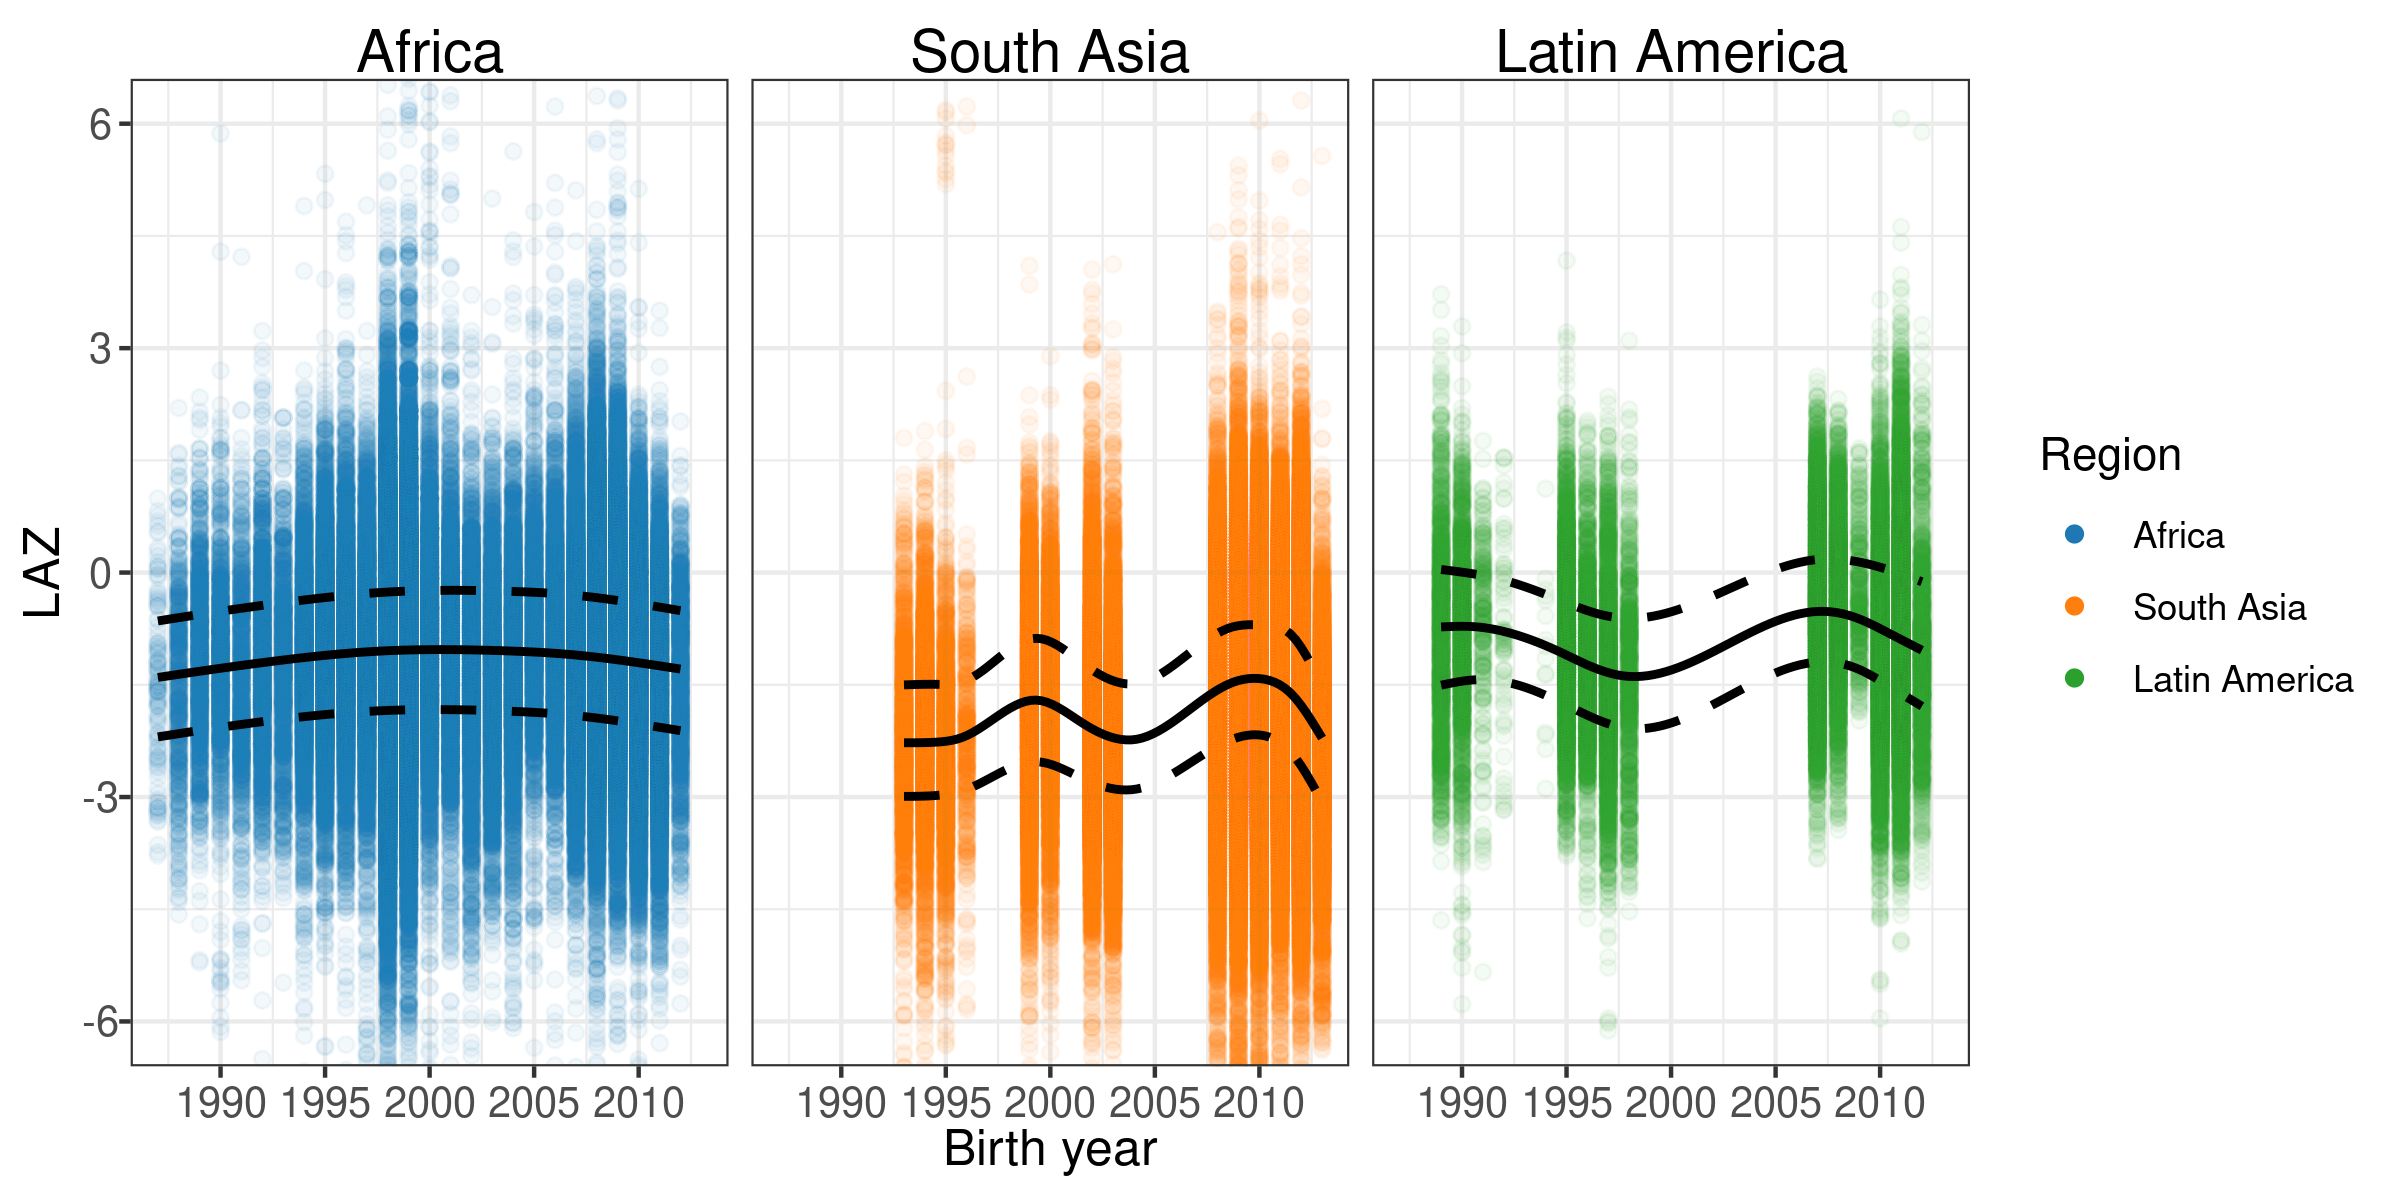
\includegraphics[width=33.33in]{figures//shared/laz_secular_trend}

\hypertarget{age-meas}{%
\chapter{Analyses of age at first measurement}\label{age-meas}}

\raggedright

Our analyses of stunting incidence assumed that children whose first measurement occurred after birth were assumed to have experienced stunting onset at the age halfway between birth and the first measurement. To assess the extent to which this assumption influenced our estimates, we plotted the distribution of age at first measurement and the age at enrollment. The vast majority of children were enrolled close to birth, and the majority were less than 5 days of age at their first measurement.

\hypertarget{histogram-of-first-measurement-within-age-0-30-days}{%
\section{Histogram of first measurement within age 0-30 days}\label{histogram-of-first-measurement-within-age-0-30-days}}

\hypertarget{all-cohorts}{%
\subsection{All cohorts}\label{all-cohorts}}

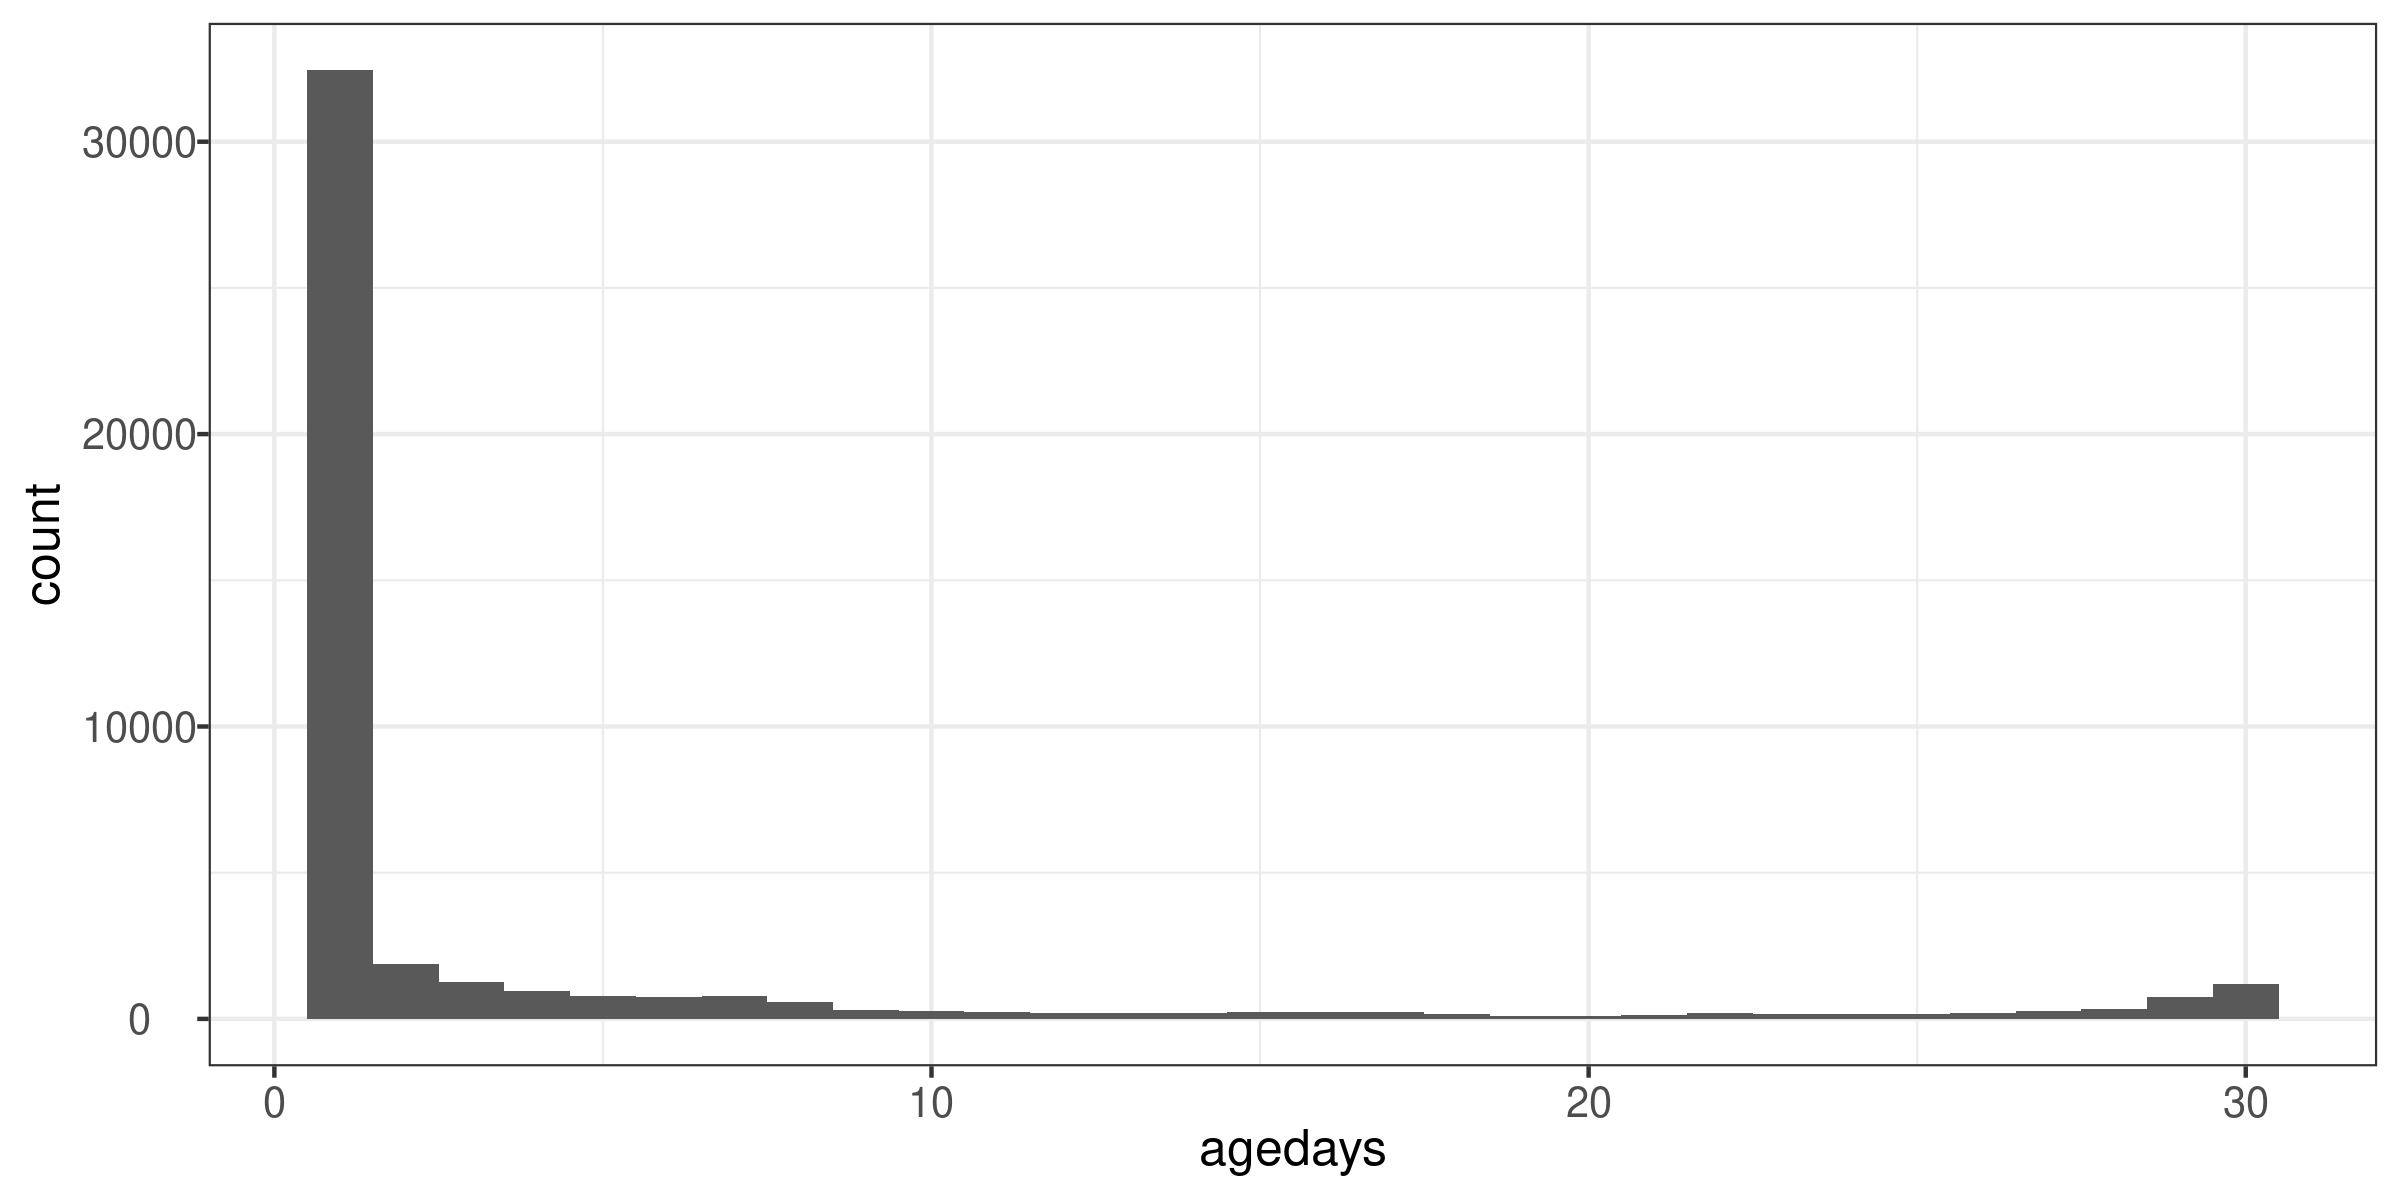
\includegraphics[width=33.33in]{figures//shared/age_histogram_first_month}

\hypertarget{cohort-stratified}{%
\subsection{Cohort-stratified}\label{cohort-stratified}}

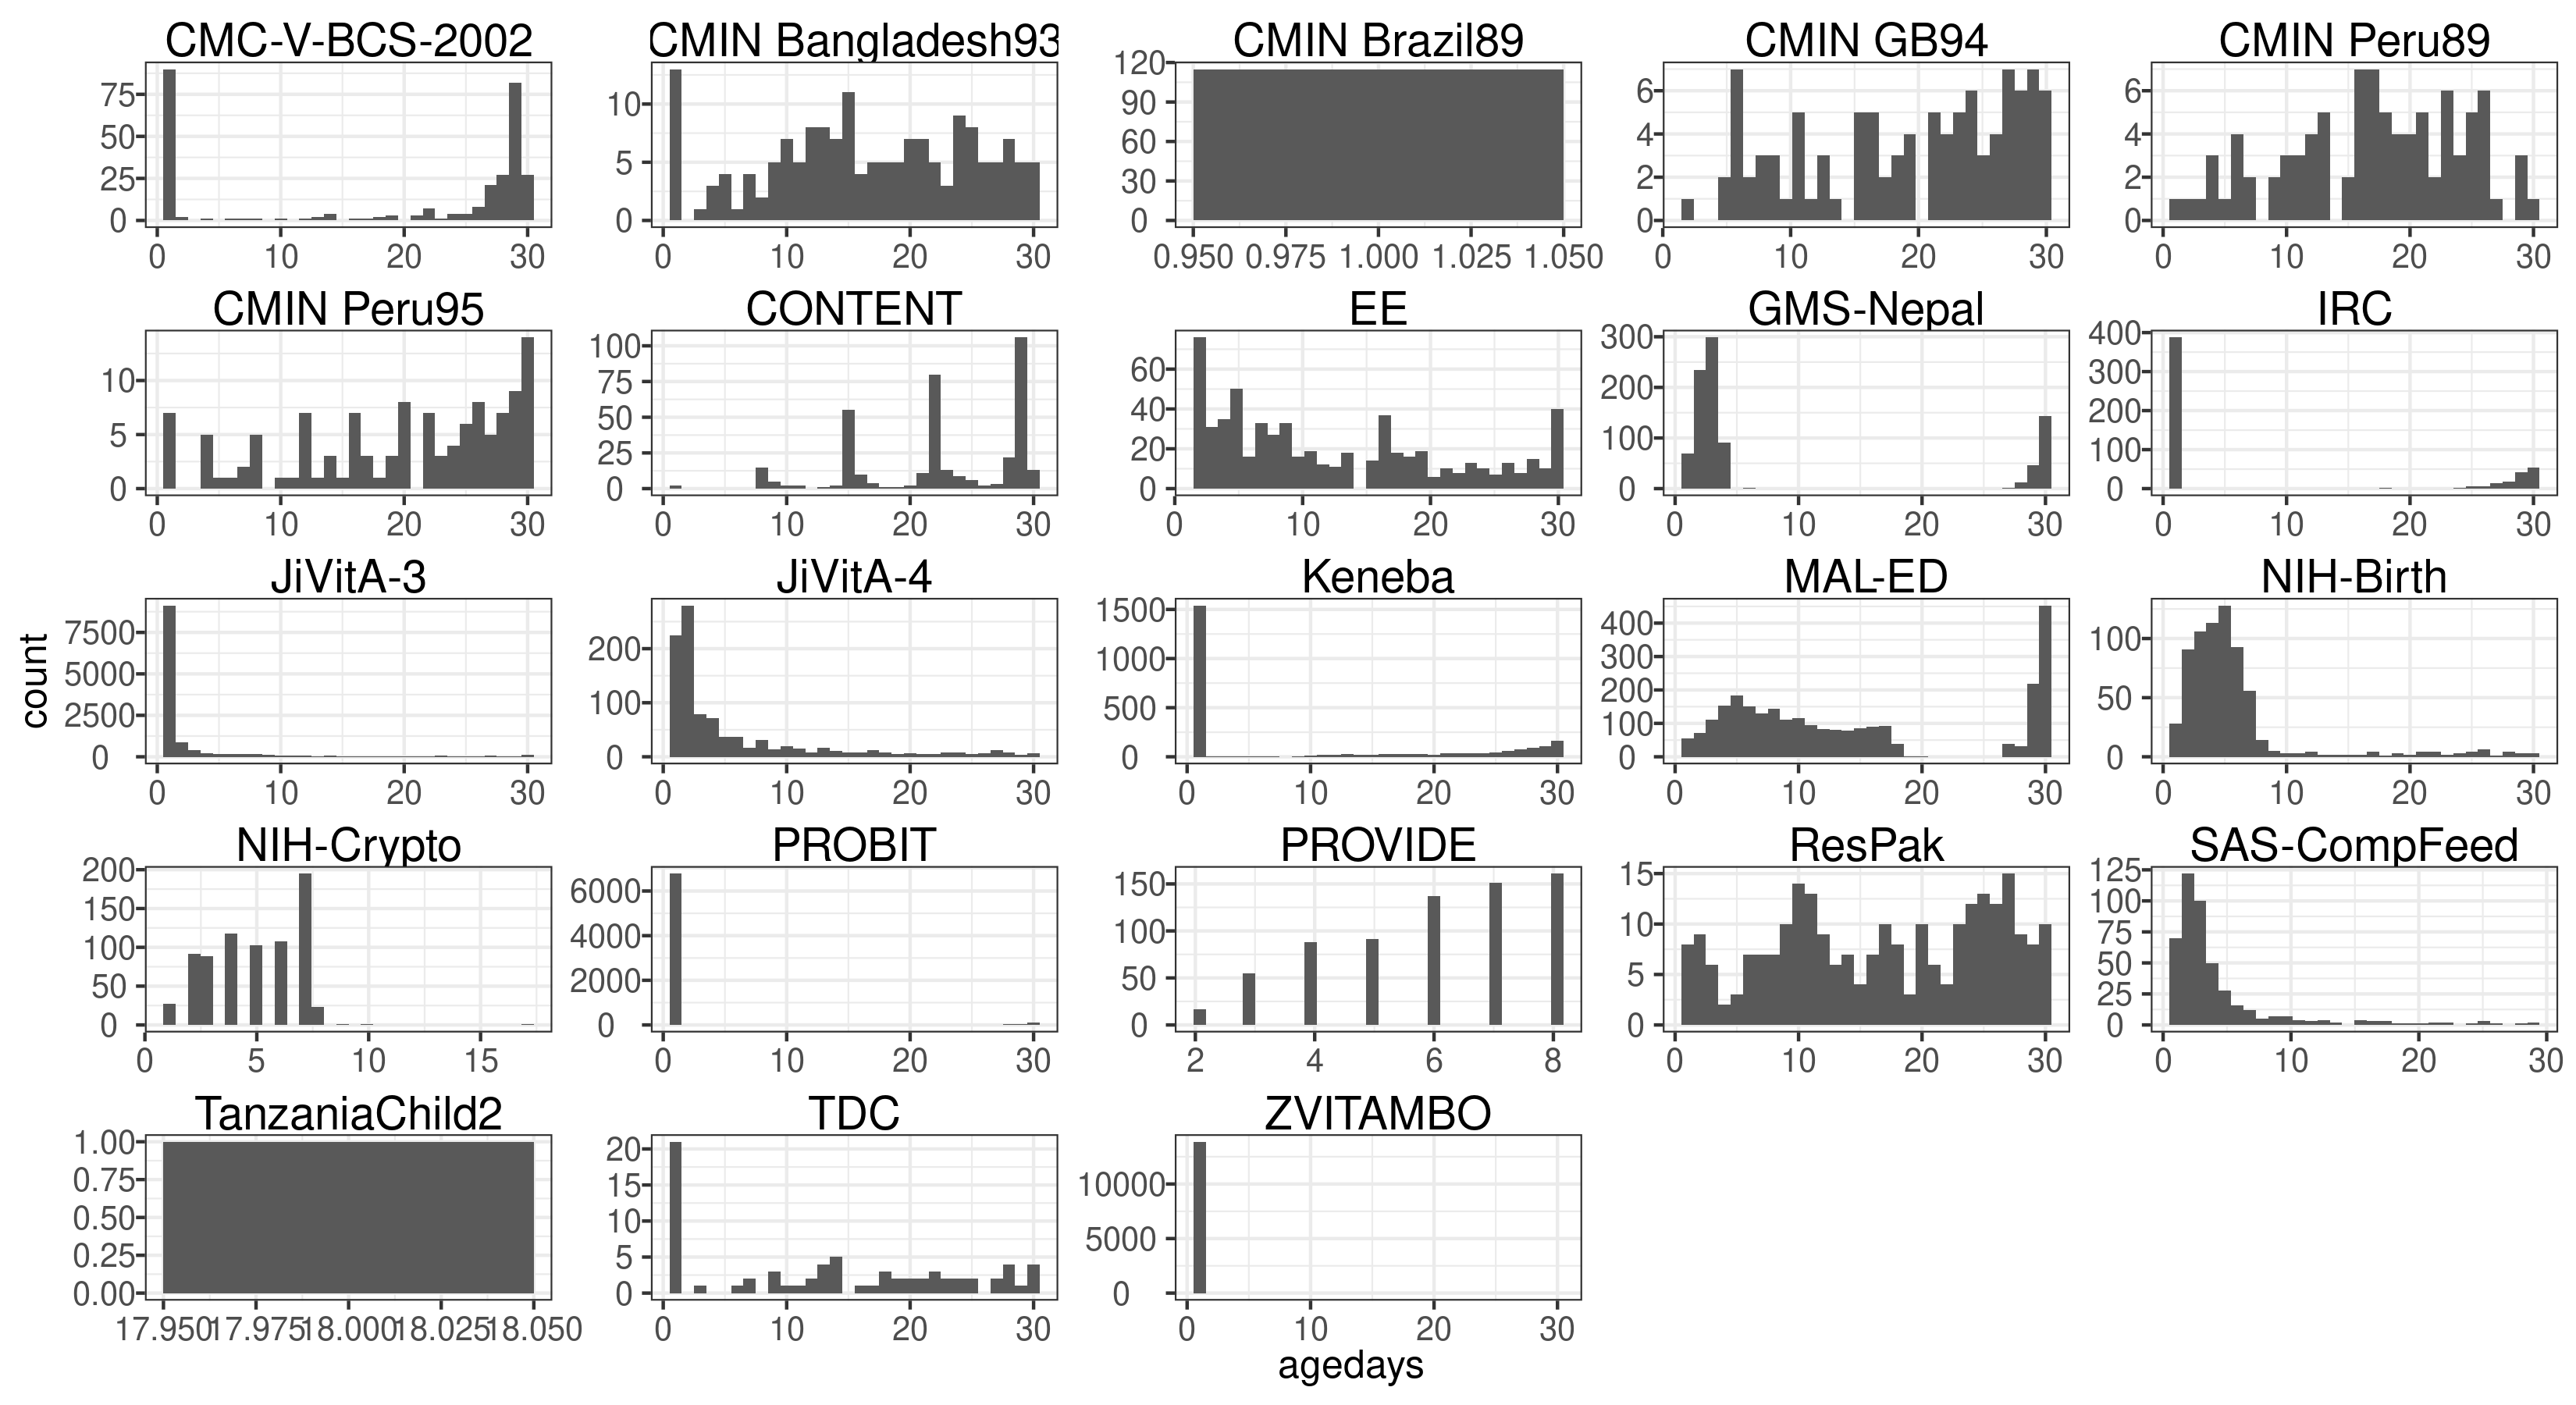
\includegraphics[width=45.83in]{figures//shared/age_histogram_first_month_cohort}

\hypertarget{histogram-of-age-at-enrollment}{%
\section{Histogram of age at enrollment}\label{histogram-of-age-at-enrollment}}

\hypertarget{all-cohorts-1}{%
\subsection{All cohorts}\label{all-cohorts-1}}

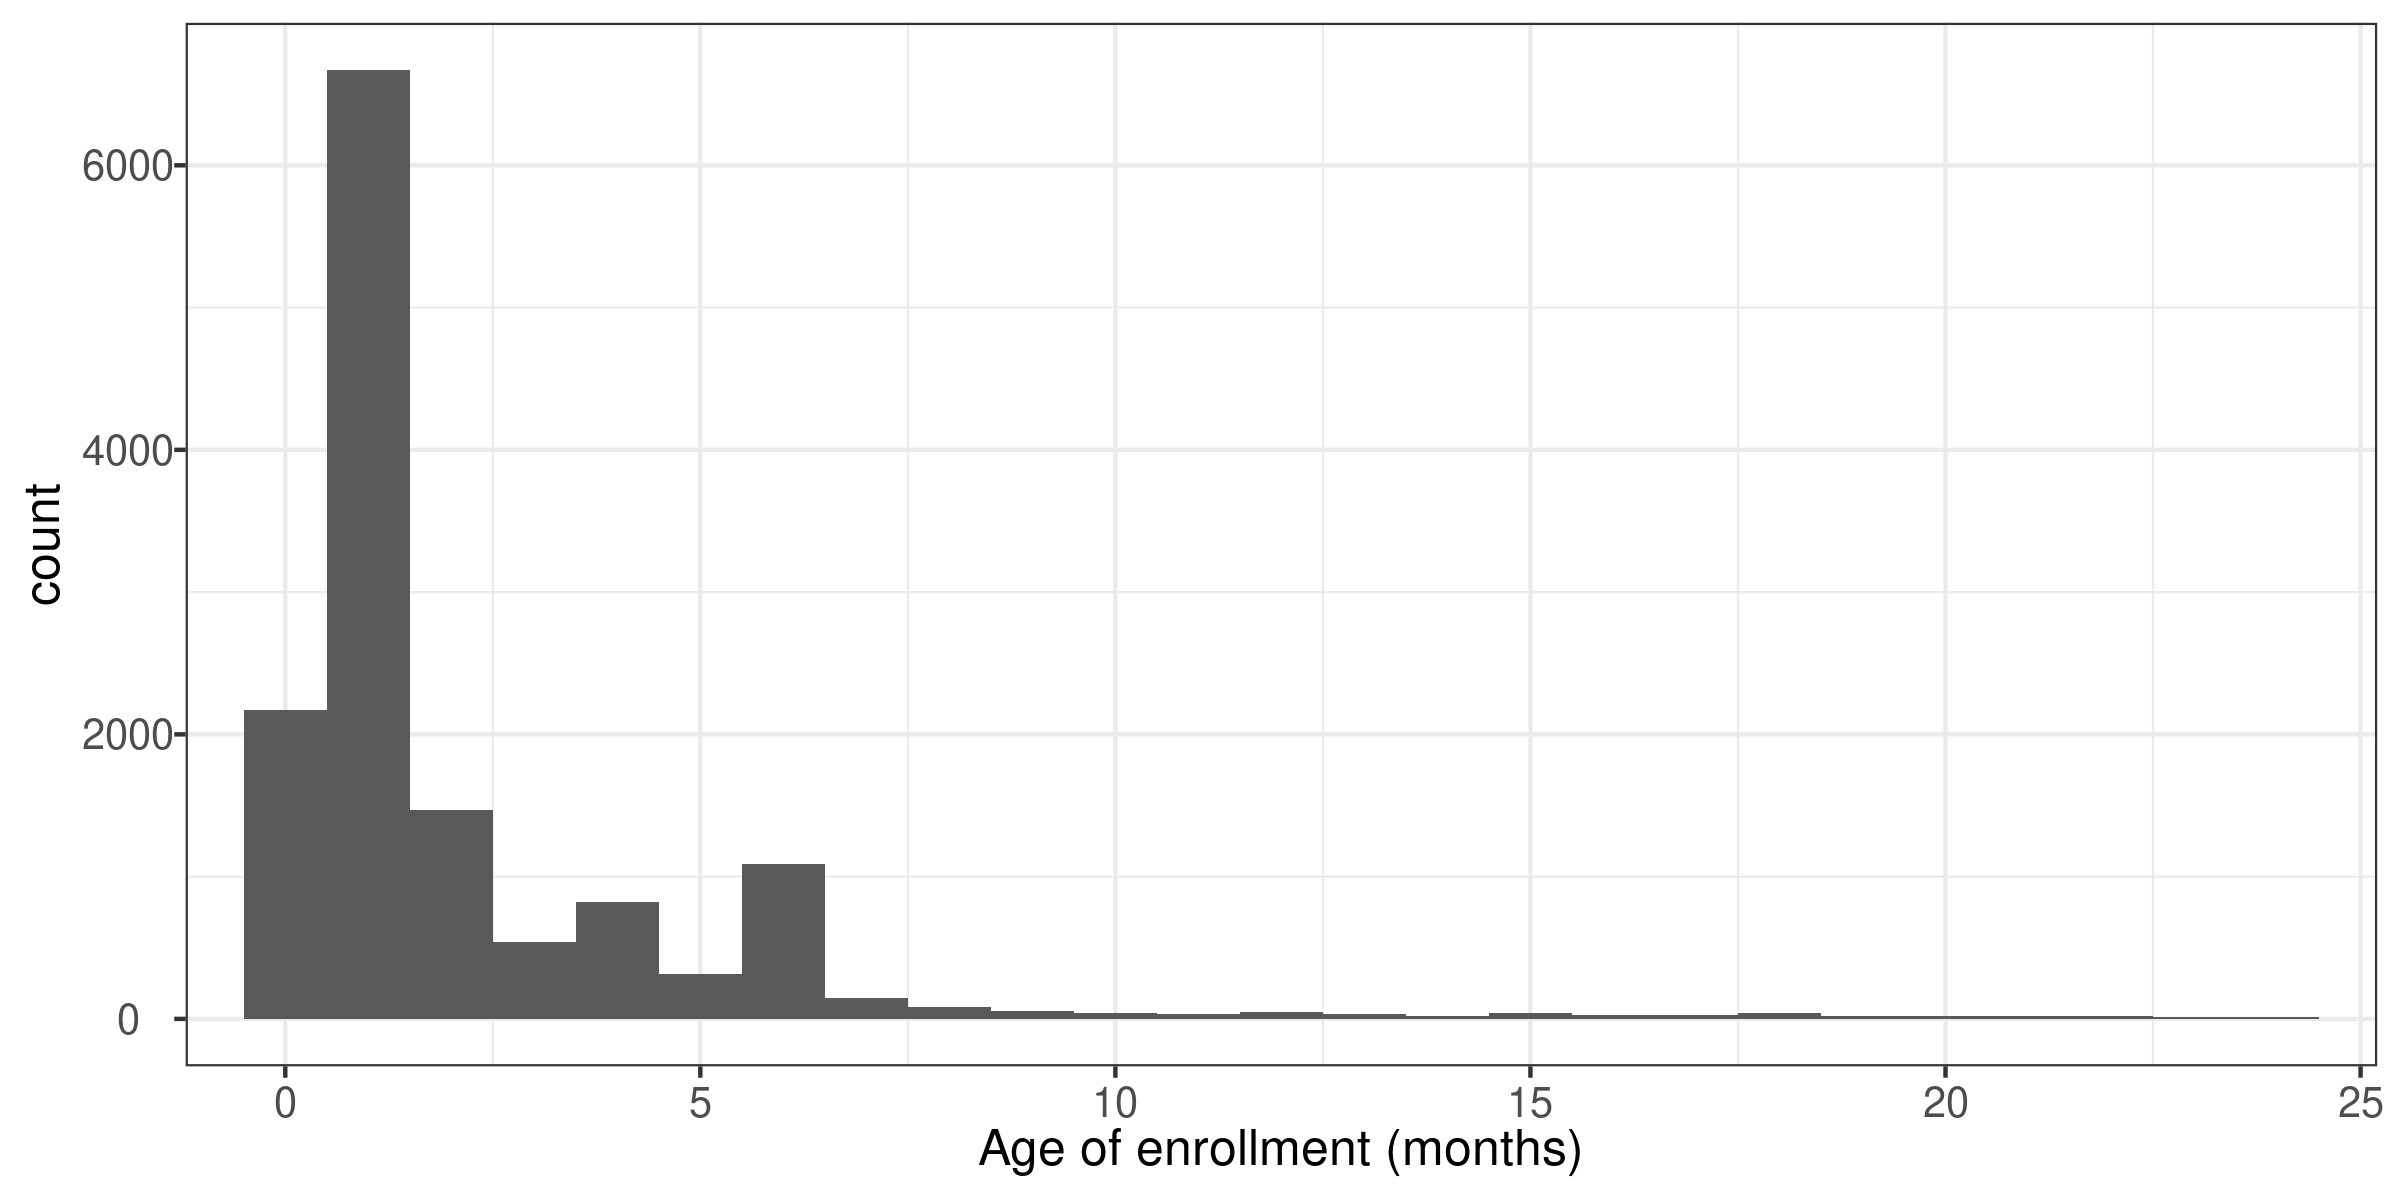
\includegraphics[width=33.33in]{figures//shared/enrollment_age_histogram_over_7d}

\hypertarget{cohort-stratified-1}{%
\subsection{Cohort-stratified}\label{cohort-stratified-1}}

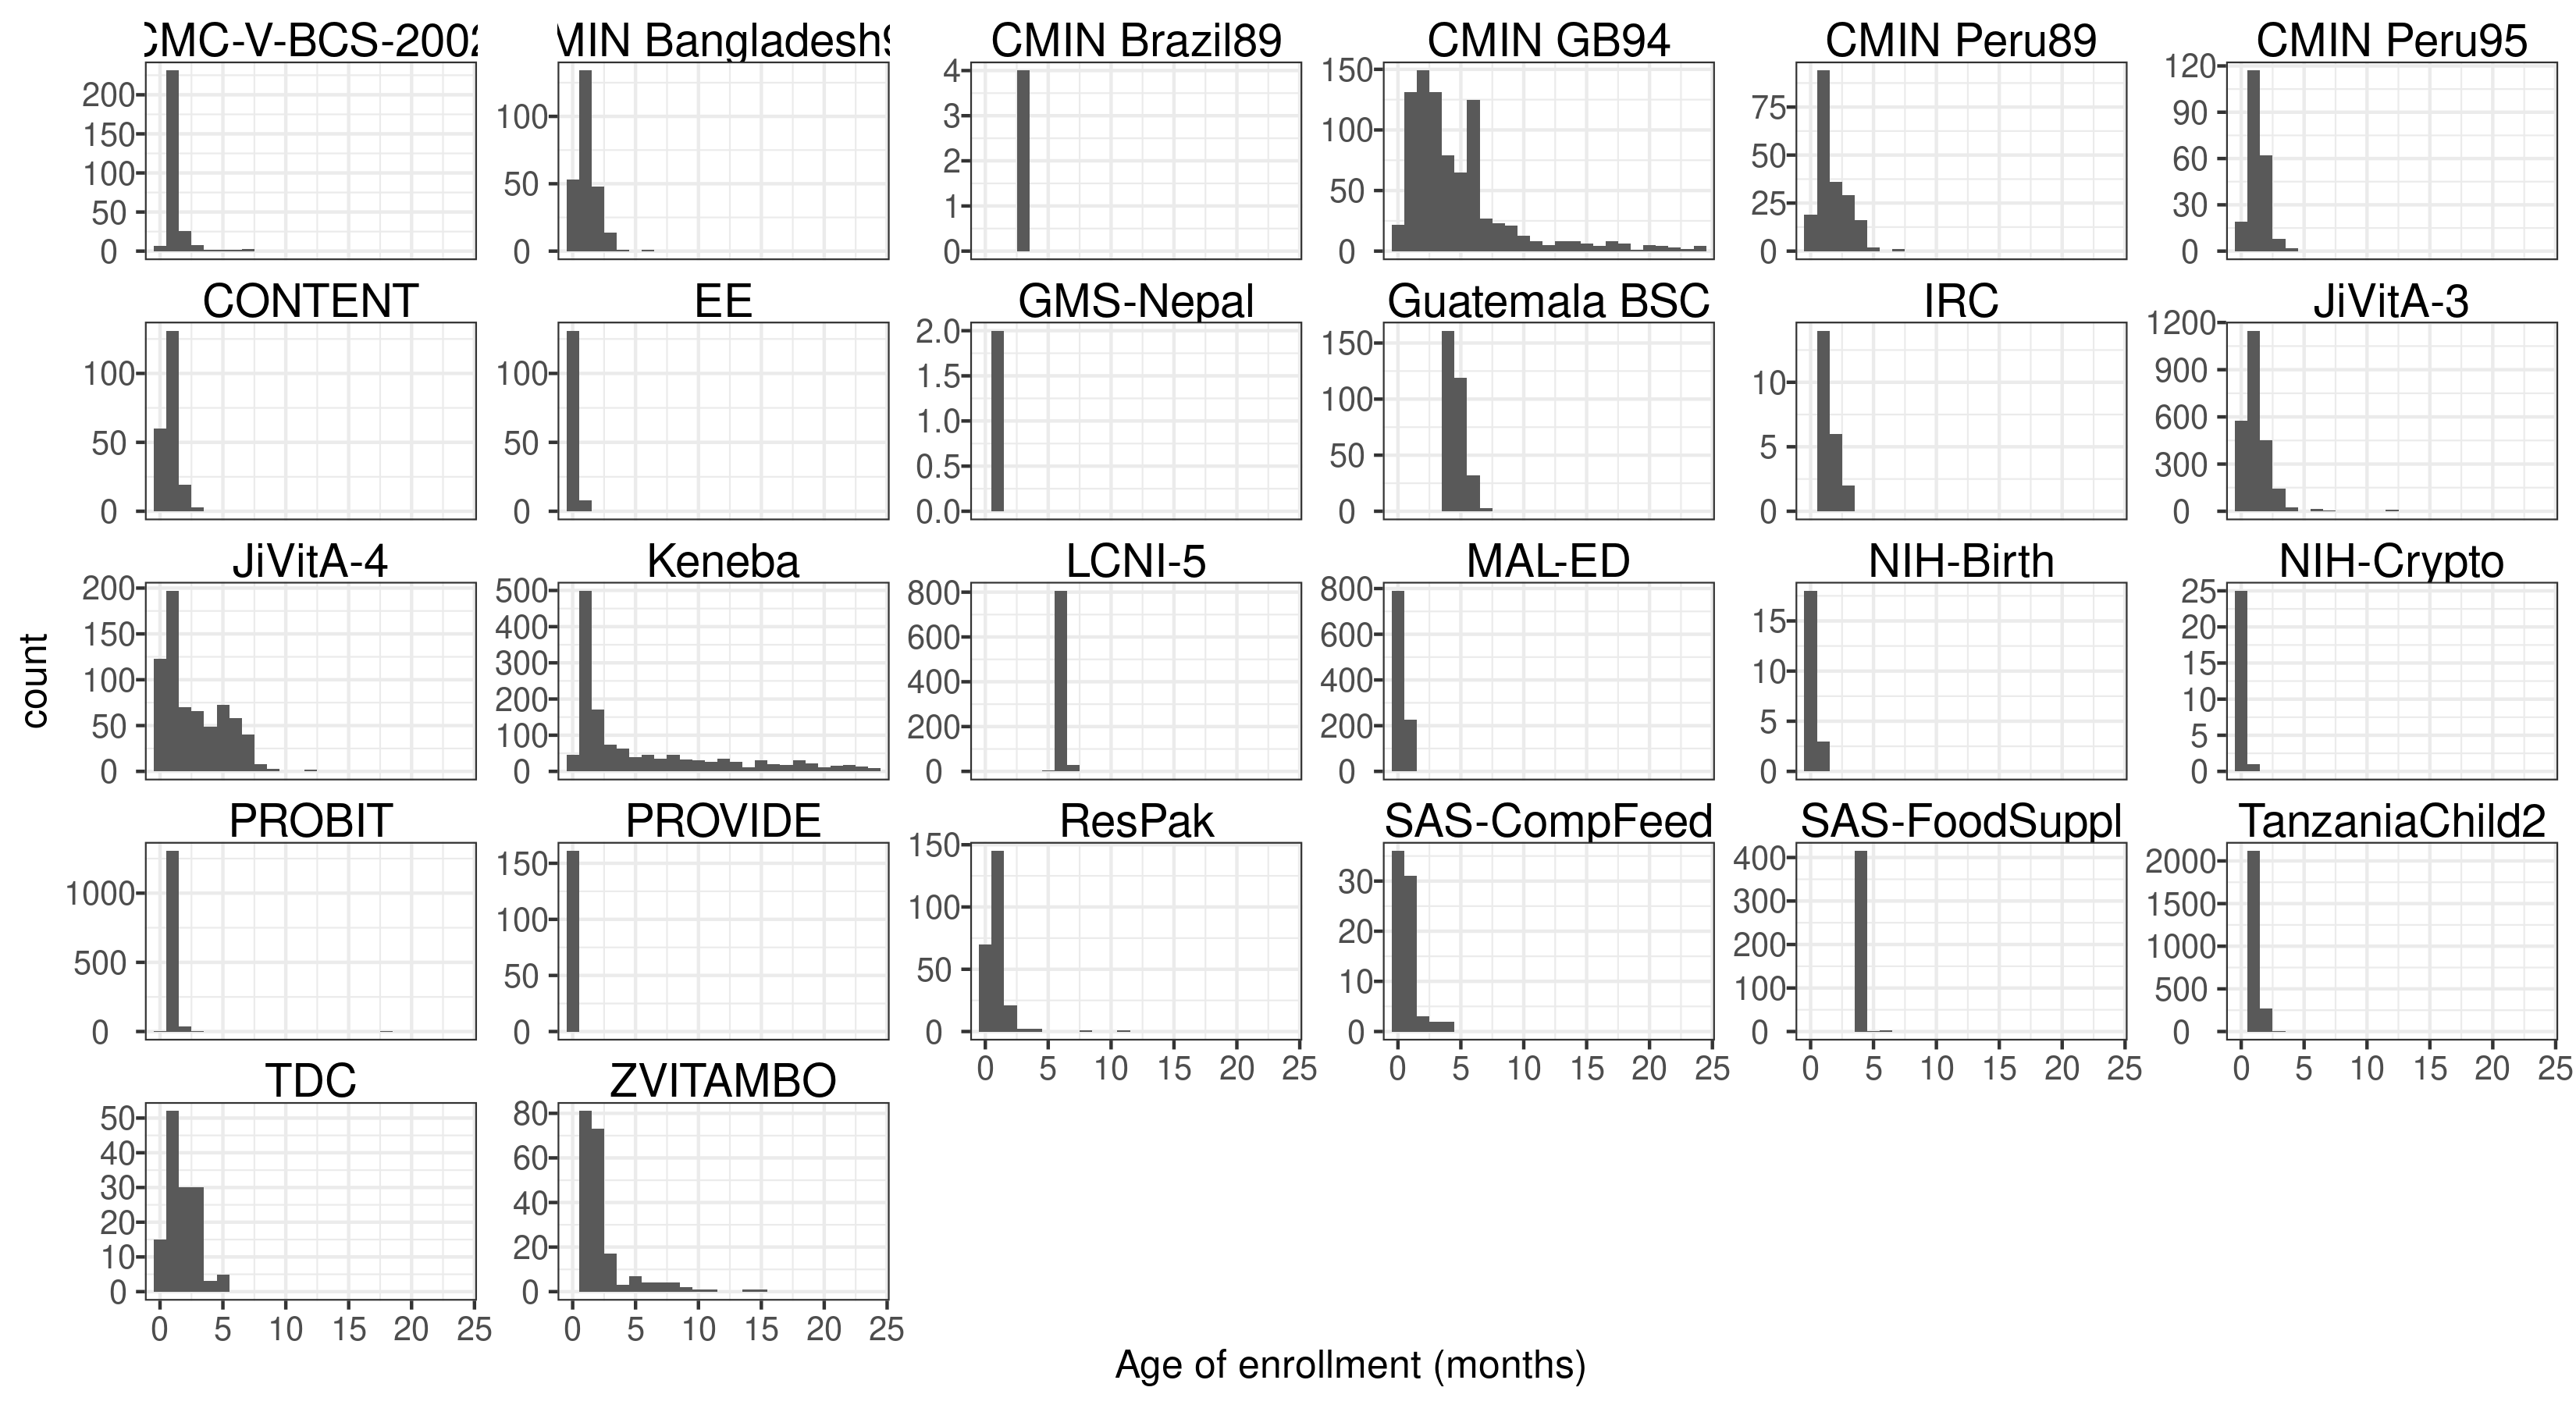
\includegraphics[width=45.83in]{figures//shared/enrollment_age_histogram_over_7d_cohort}

\hypertarget{DHS}{%
\chapter{Comparison to DHS surveys from matching countries}\label{DHS}}

\raggedright

In the manuscript, we compared the mean length-for-age Z-score by age and region in our included studies and in Demographic and Health Survey (DHS) datasets from the same countries as those included in our study. Here we present analogous plots including all of the countries from each region. The plots are kernel density distributions of length-for-age z-scores (LAZ) in Demographic and Health Survey (DHS) datasets (dashed lines) and ki cohorts (solid lines). DHS estimates use the most recent survey from all countries in each region. Open circles indicate median LAZ in ki cohorts; closed circles indicate median LAZ in DHS cohorts.

\#\#\#\#\#NEED TO UPDATE FIGURE-NOT FOUND

\hypertarget{cohort}{%
\chapter{Cohort-specific results}\label{cohort}}

\raggedright

Here, we present cohort-specific estimates of length-for-age Z-score by age, age-specific prevalence, and age-specific incidence.

\hypertarget{mean-length-for-age-z-score-by-age}{%
\section{Mean length-for-age Z-score by age}\label{mean-length-for-age-z-score-by-age}}

\hypertarget{africa}{%
\subsection{Africa}\label{africa}}

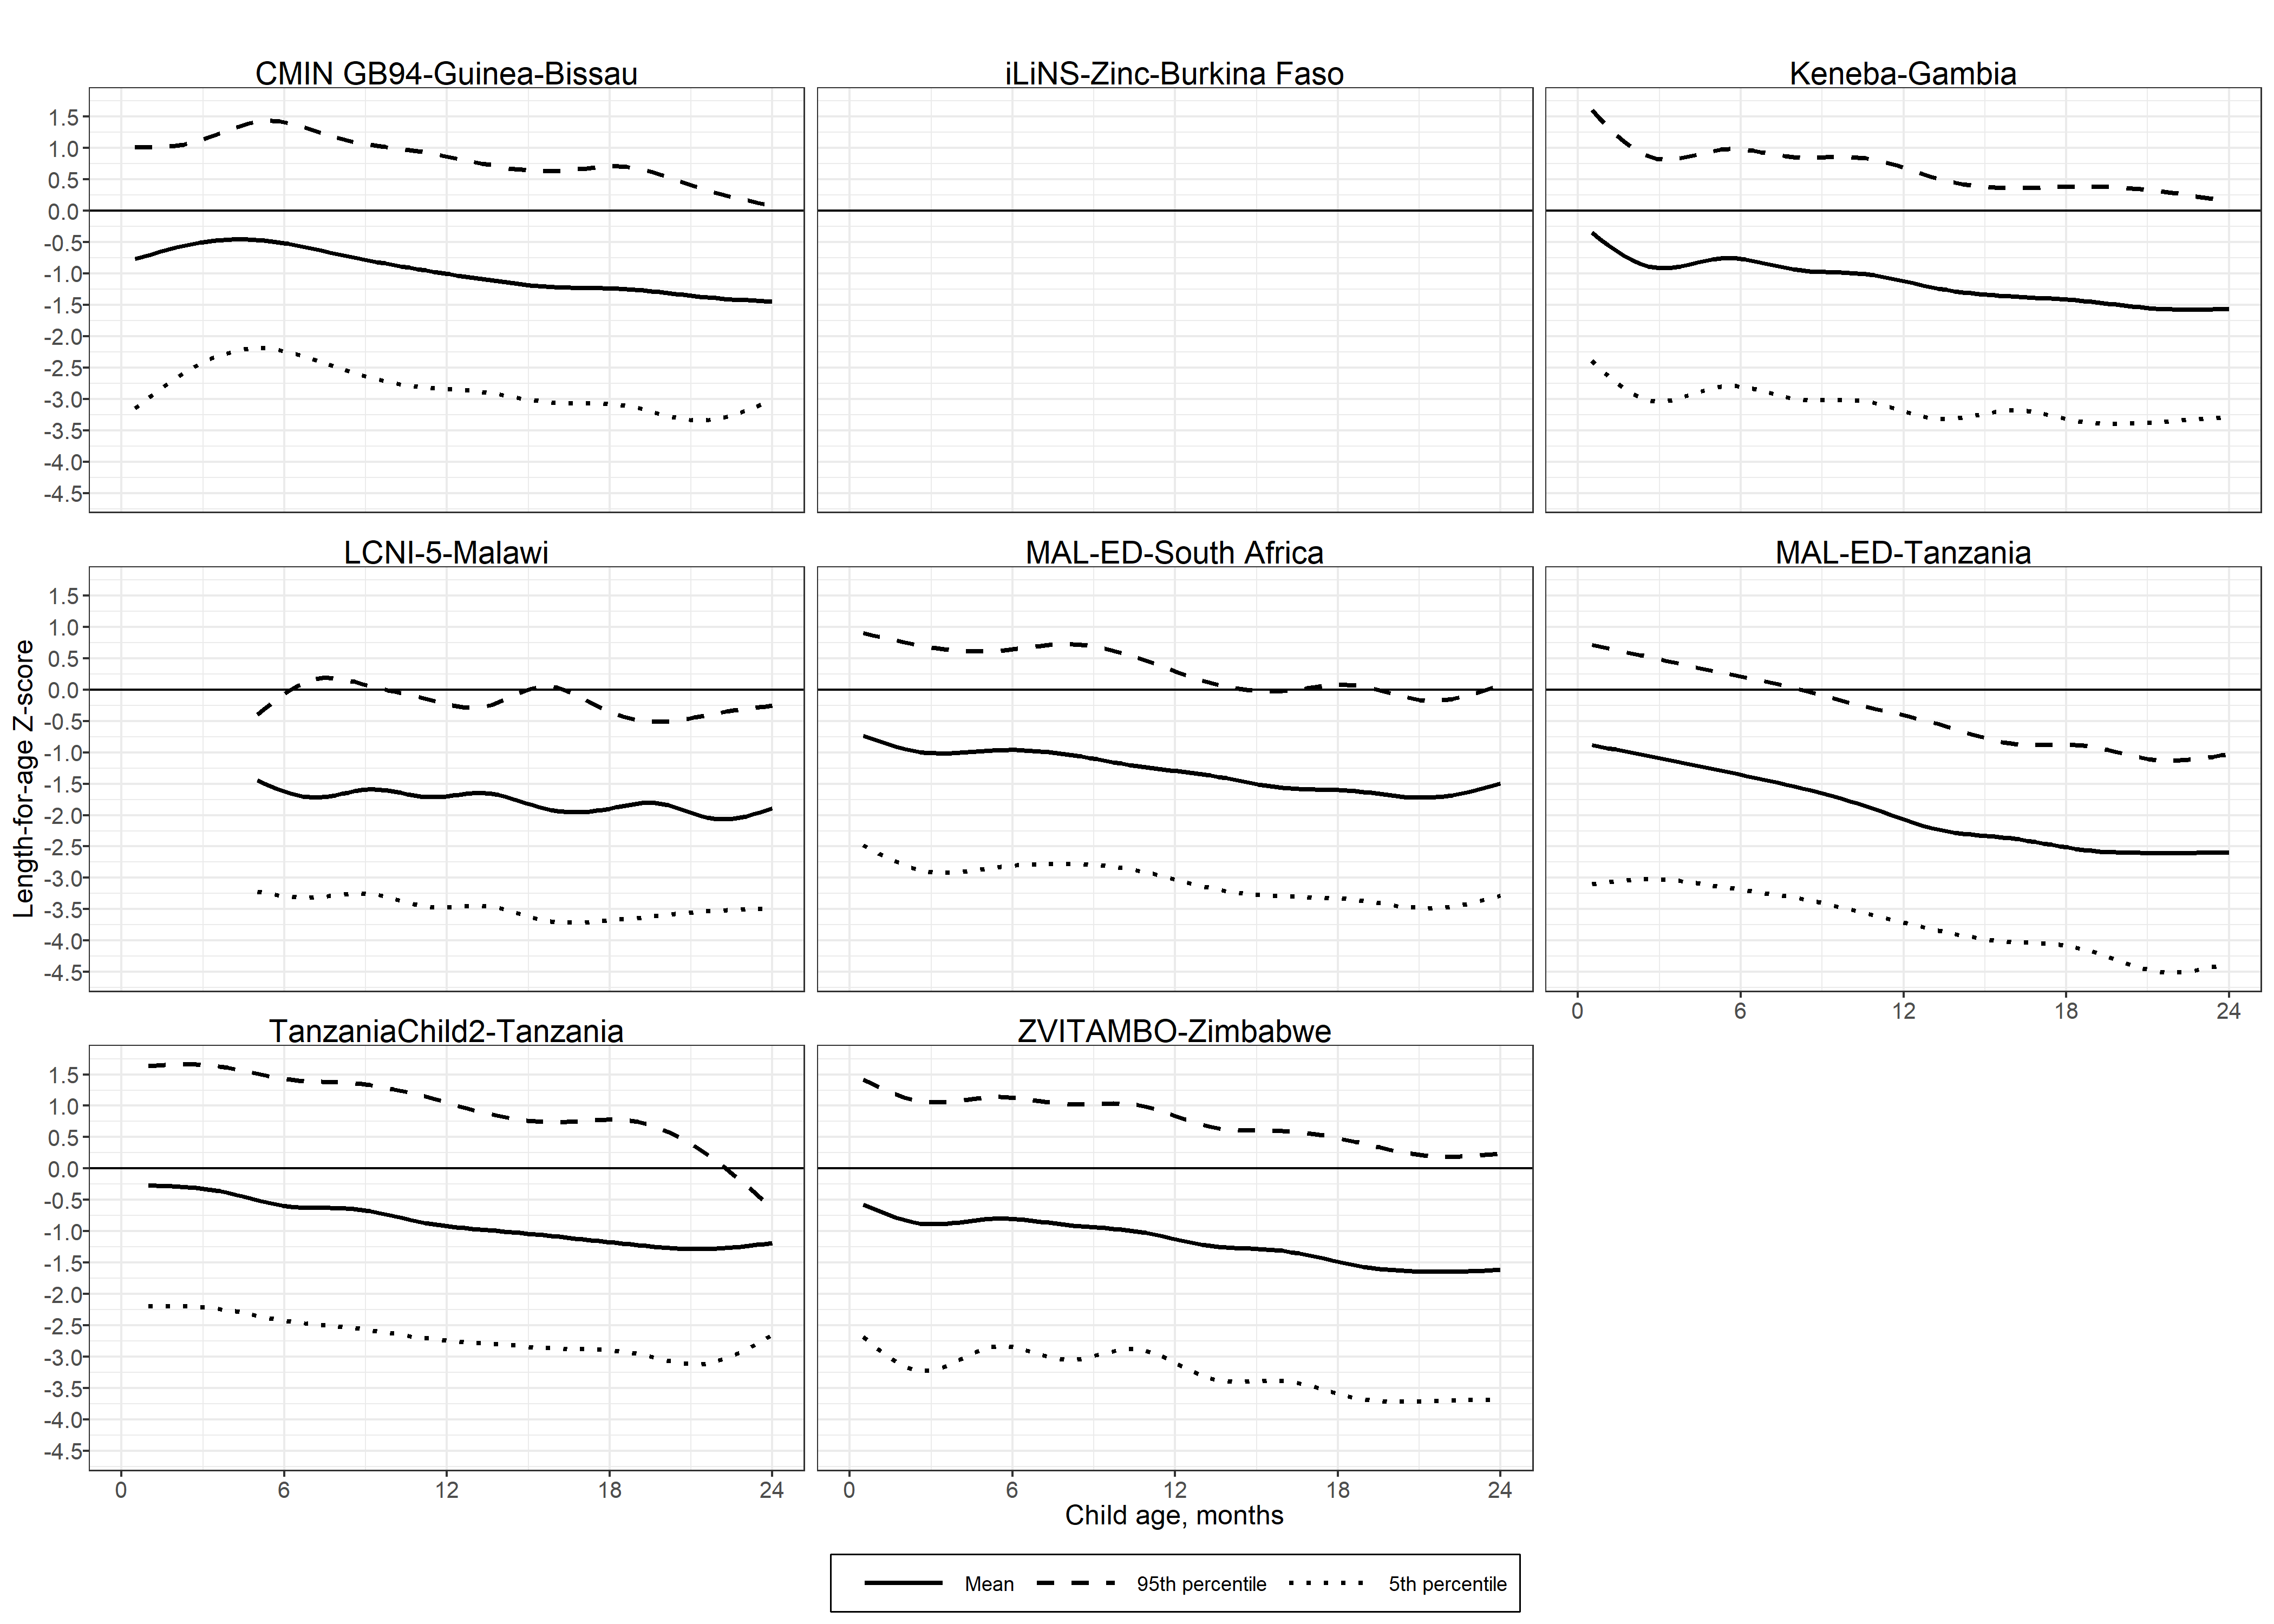
\includegraphics[width=58.33in]{figures//stunting/fig-laz-2-quant-cohort-africa-allage-primary}

\hypertarget{latin-america}{%
\subsection{Latin America}\label{latin-america}}

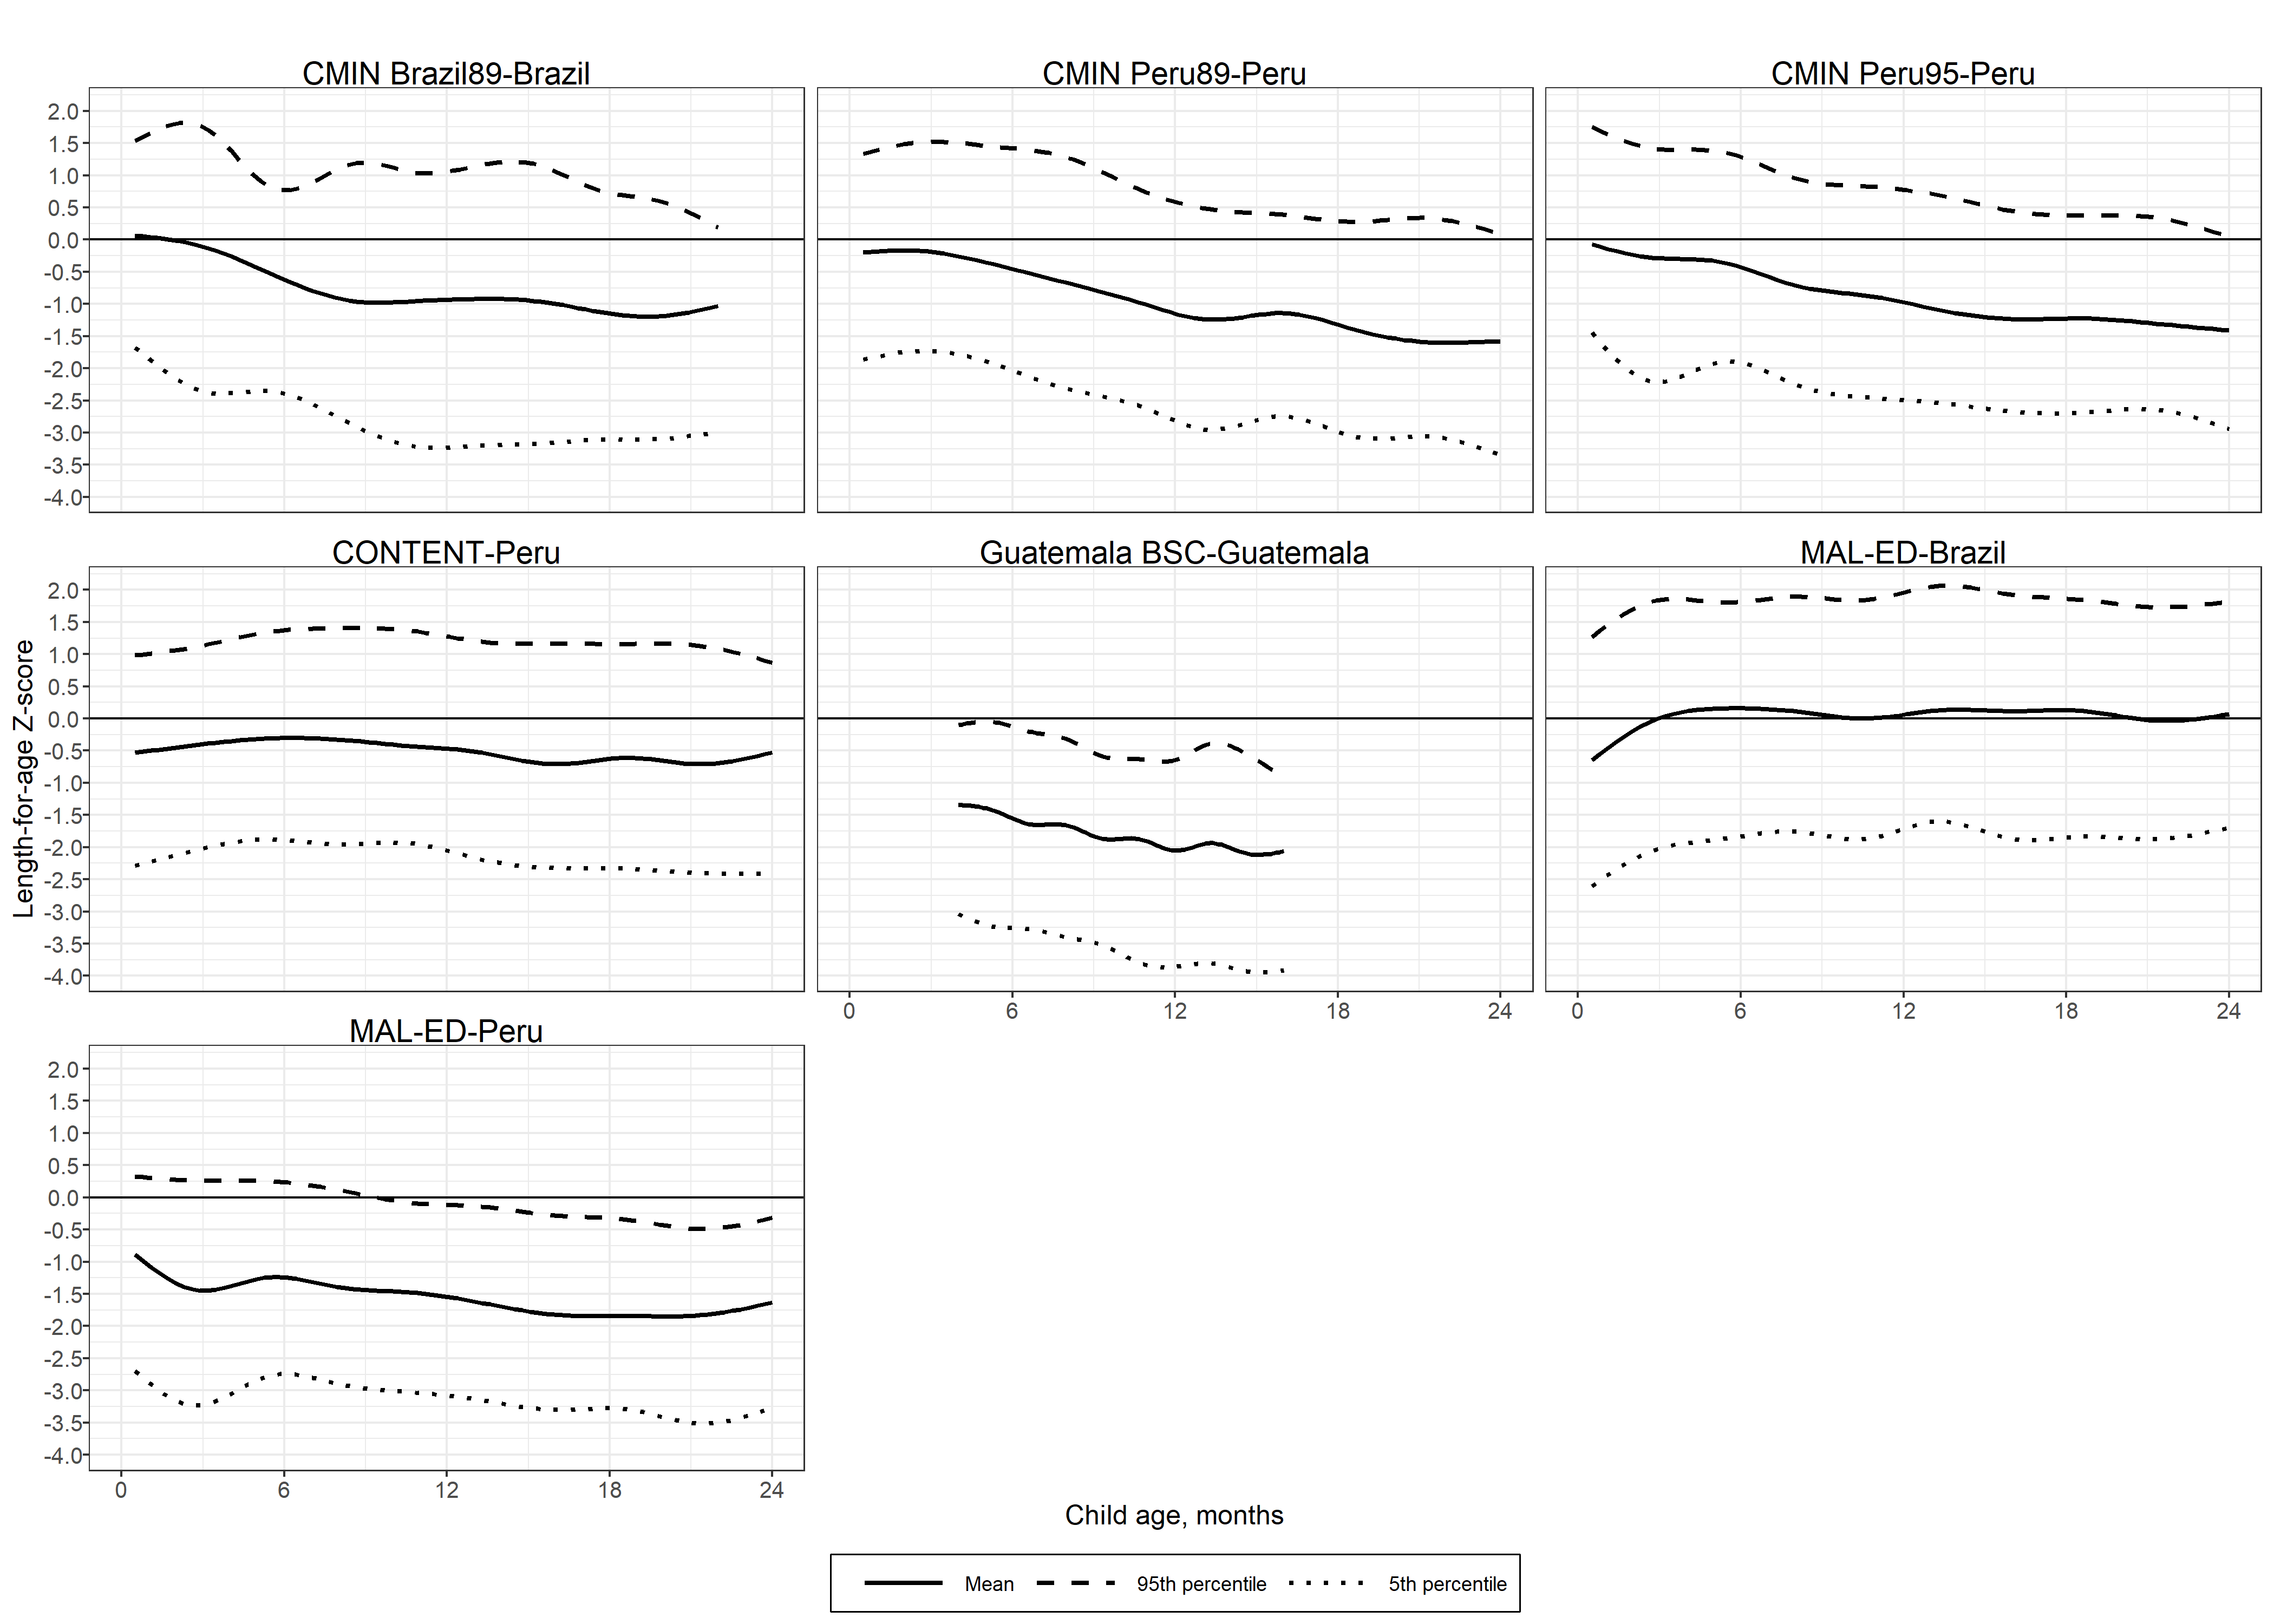
\includegraphics[width=58.33in]{figures//stunting/fig-laz-2-quant-cohort-latamer-allage-primary}

\hypertarget{south-asia}{%
\subsection{South Asia}\label{south-asia}}

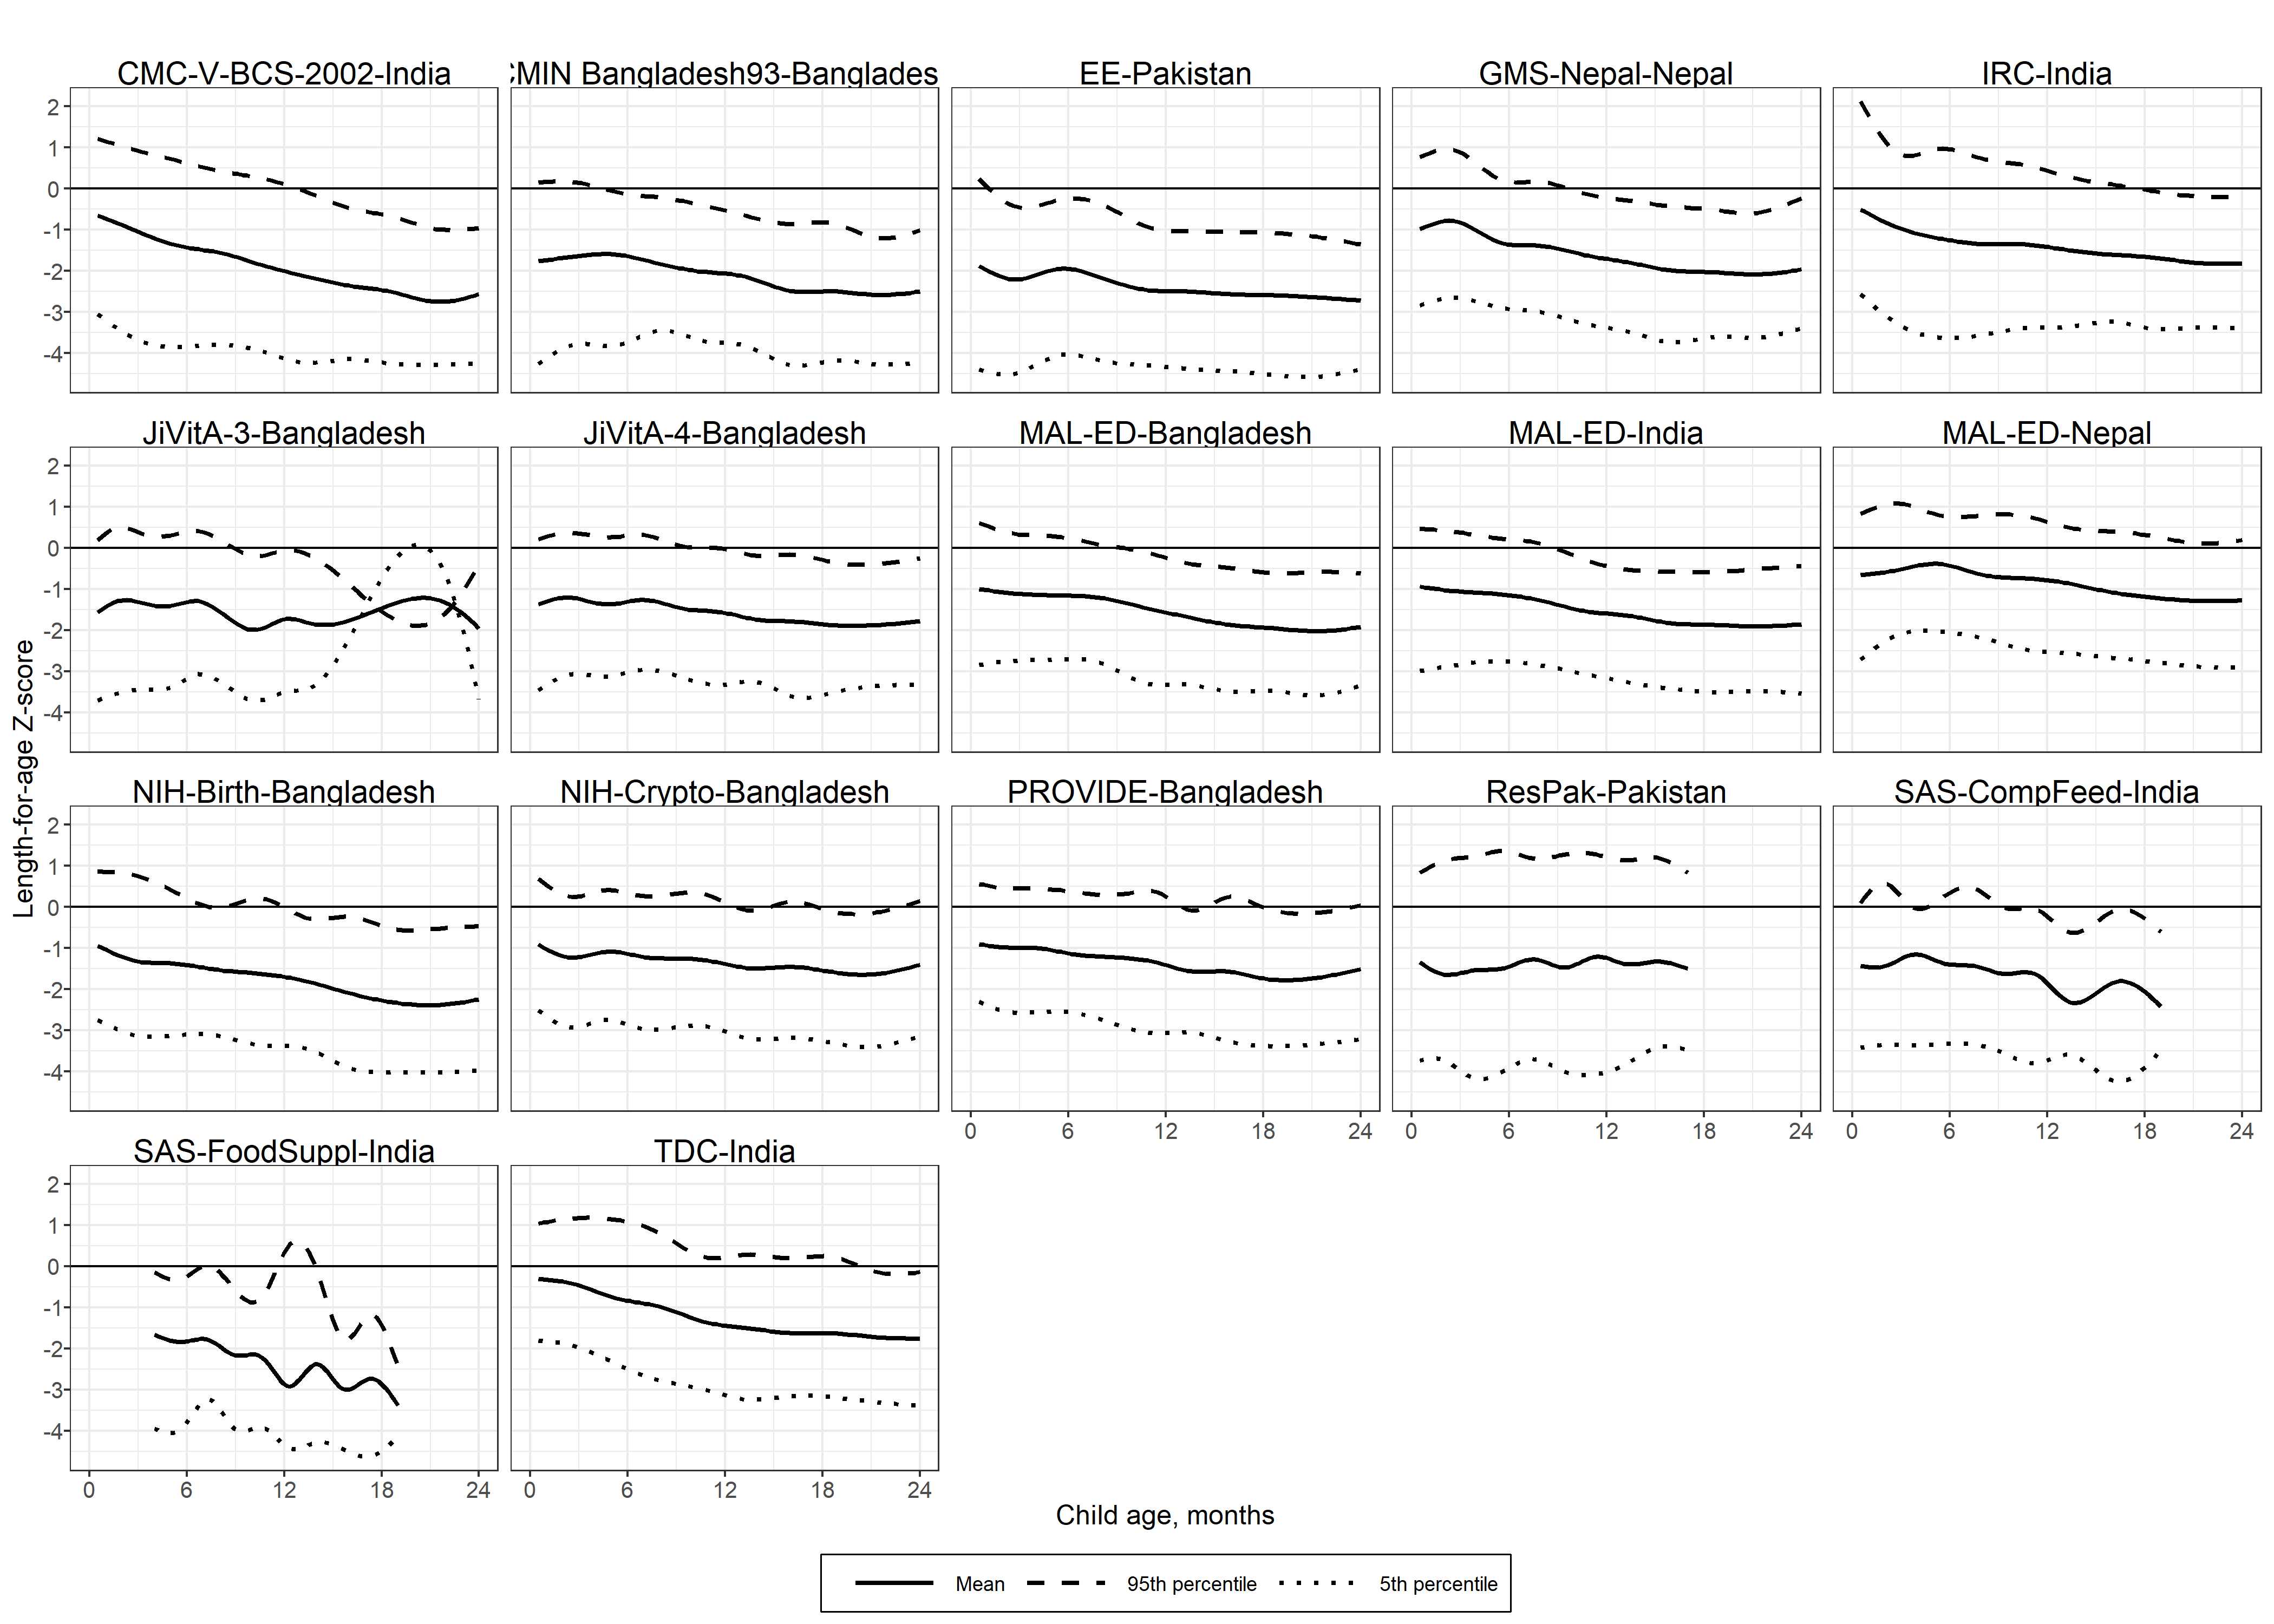
\includegraphics[width=58.33in]{figures//stunting/fig-laz-2-quant-cohort-asia-allage-primary}

\hypertarget{age-specific-prevalence}{%
\section{Age-specific prevalence}\label{age-specific-prevalence}}

\hypertarget{africa-1}{%
\subsection{Africa}\label{africa-1}}

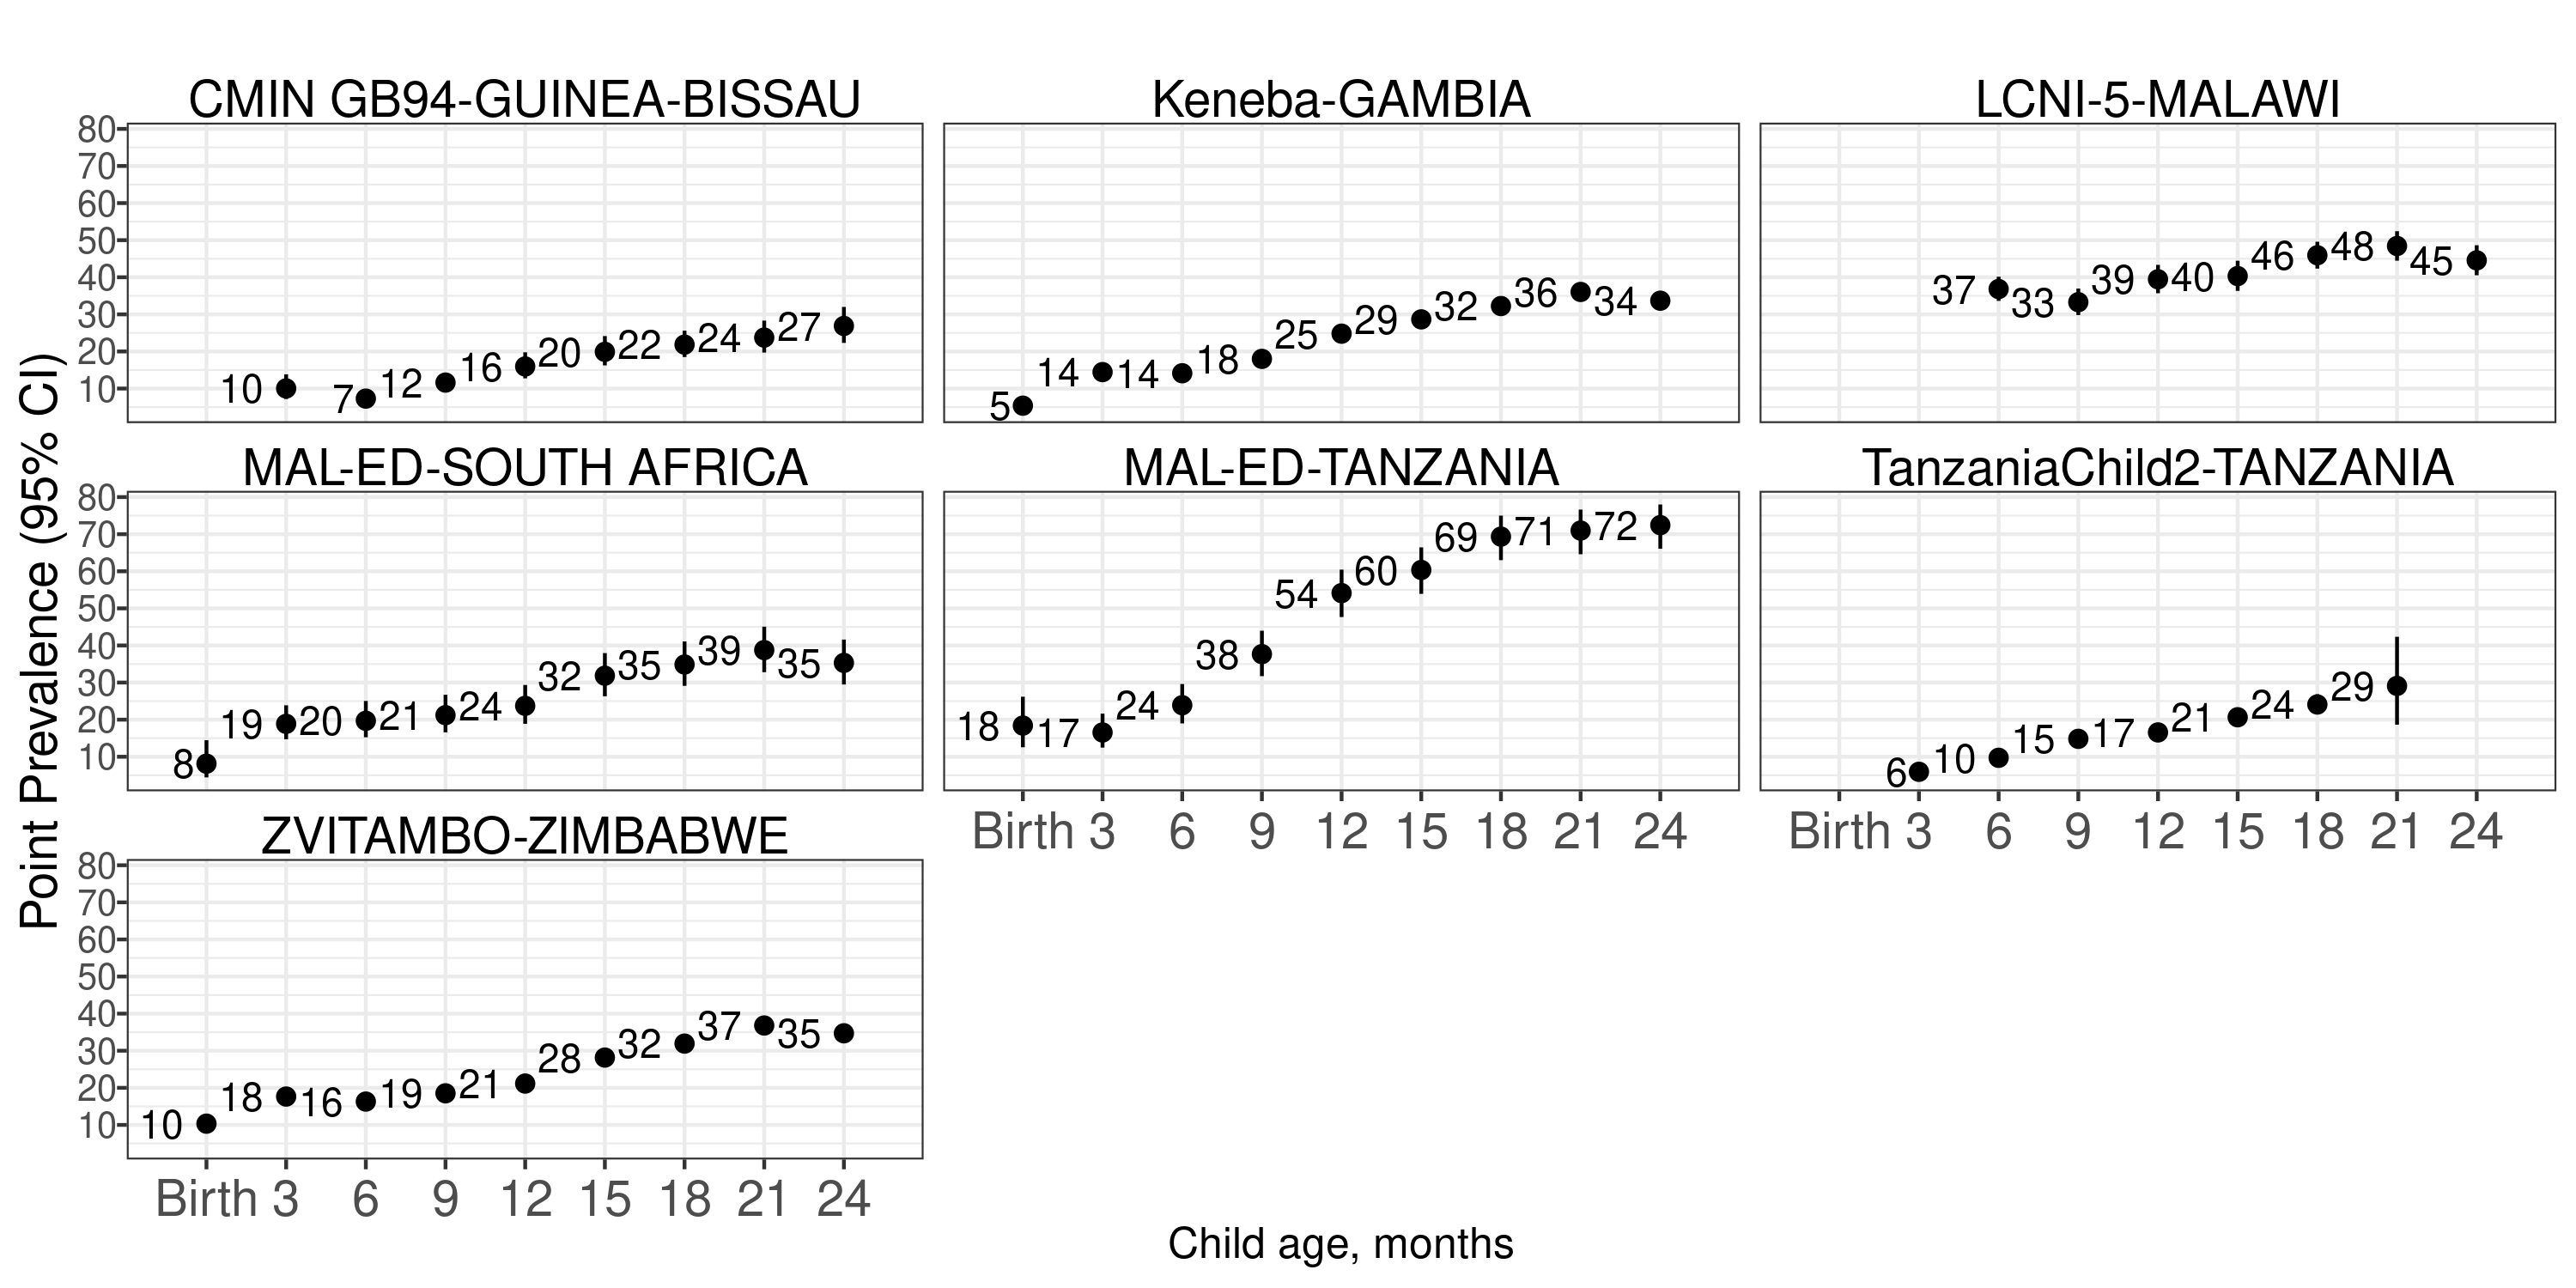
\includegraphics[width=41.67in]{figures//stunting/fig-stunt-2-prev-cohort-africa-allage-primary}

\hypertarget{latin-america-1}{%
\subsection{Latin America}\label{latin-america-1}}

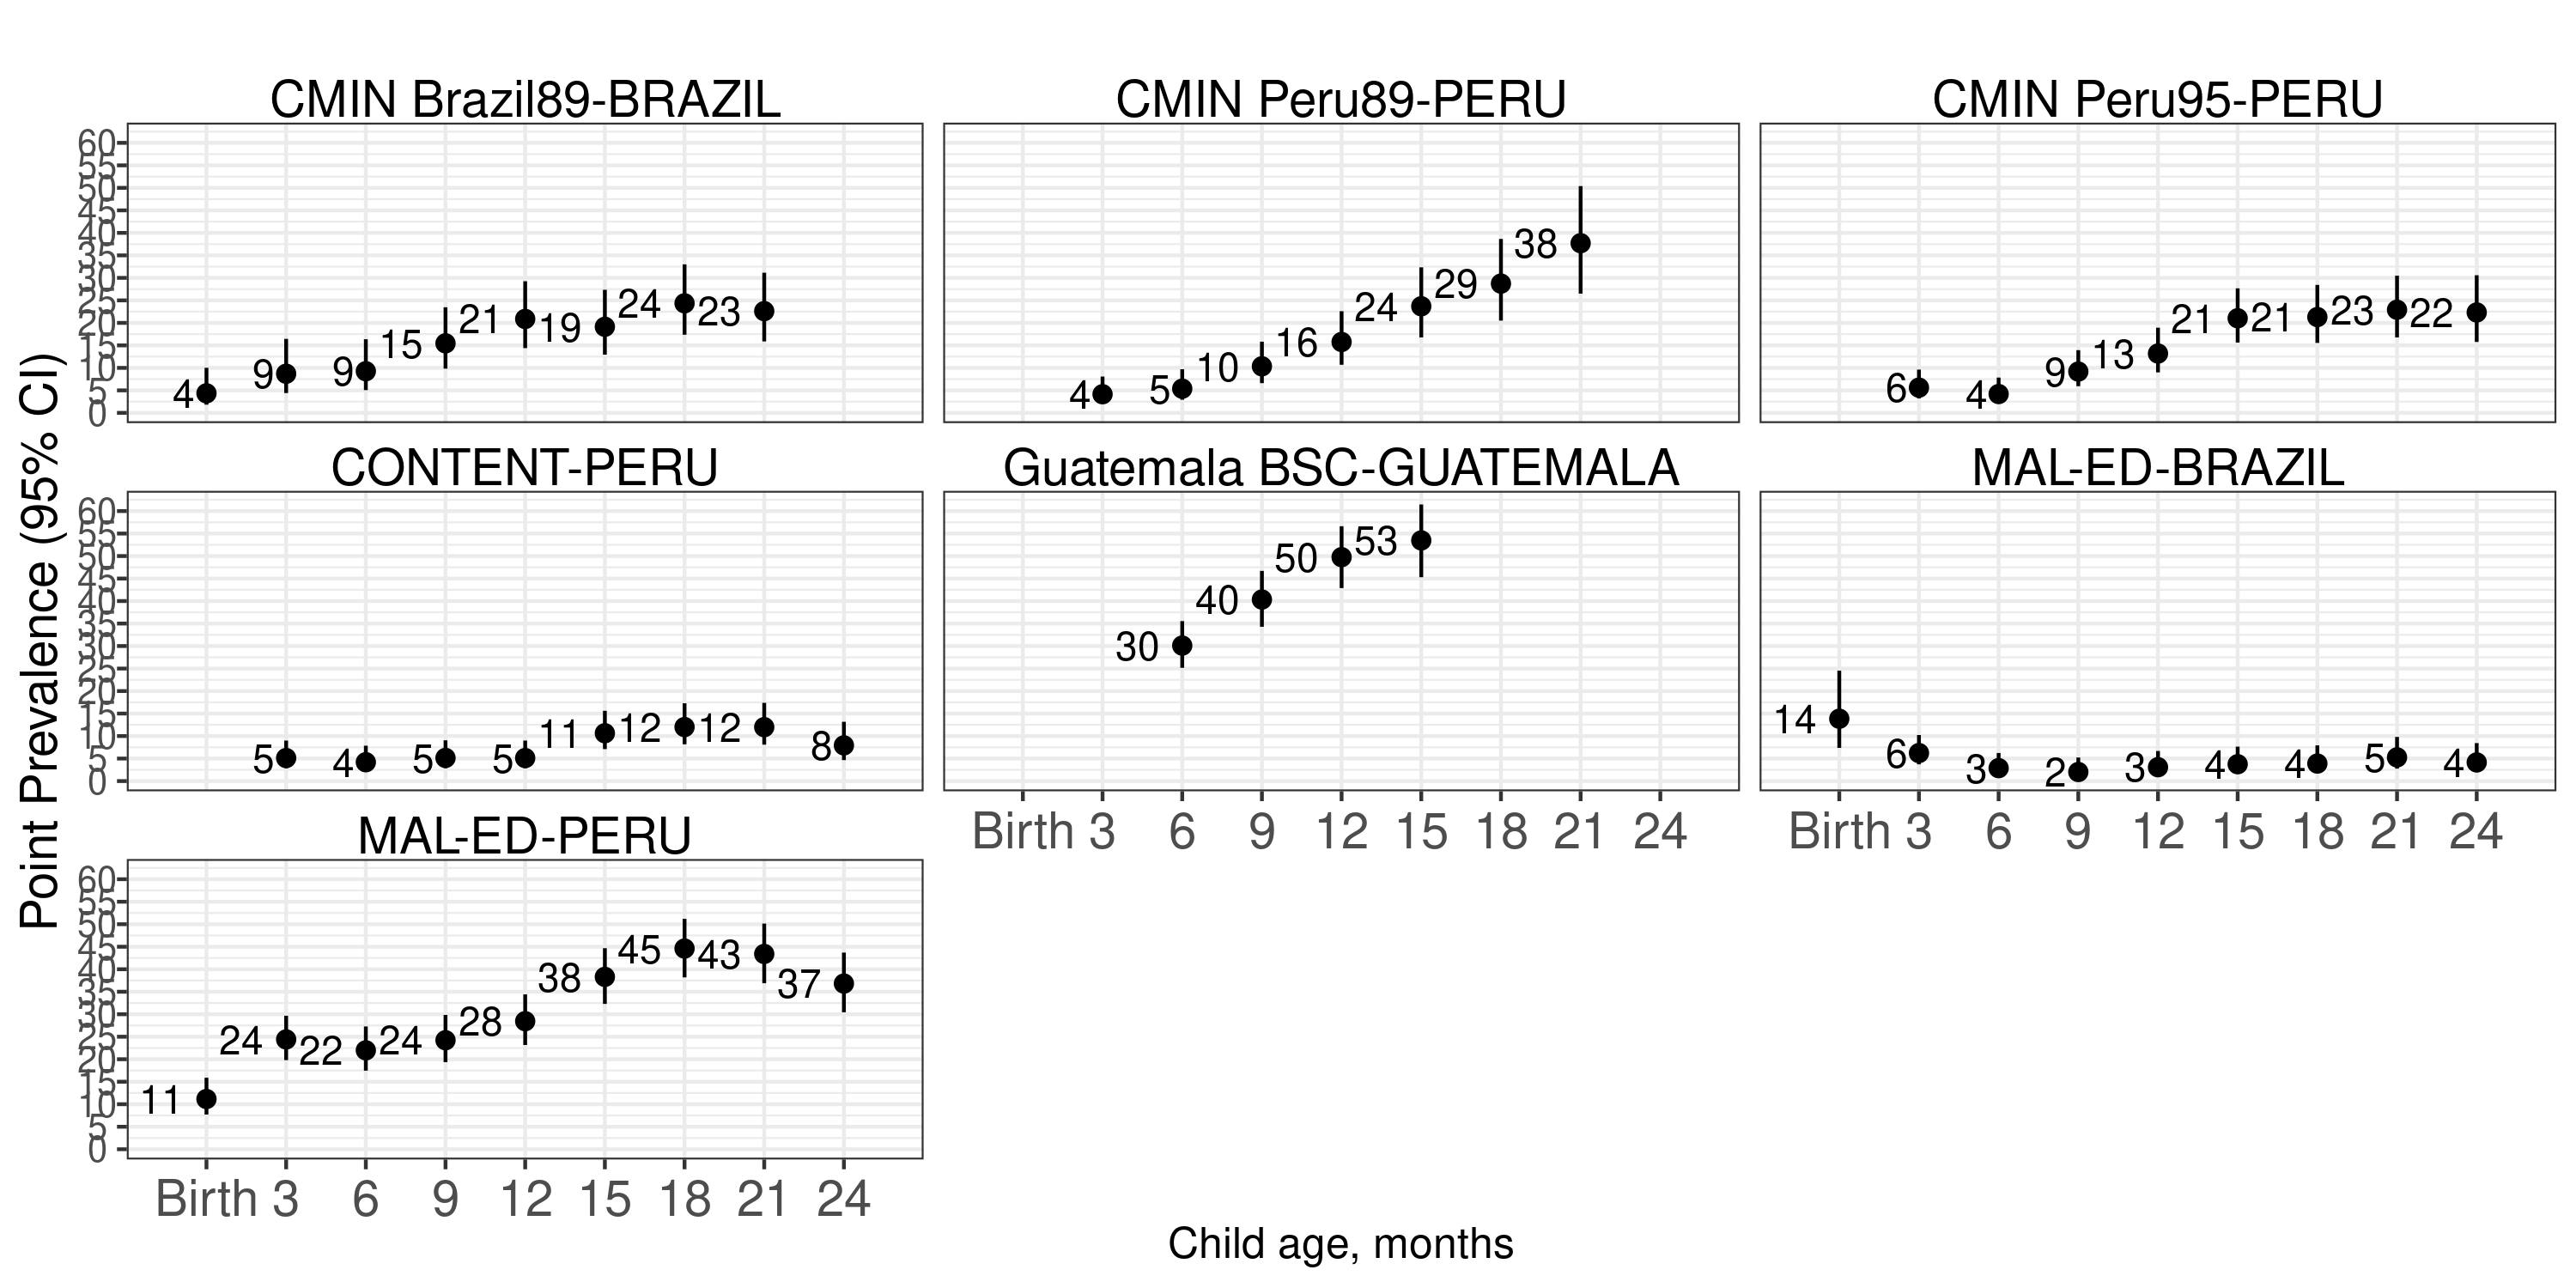
\includegraphics[width=41.67in]{figures//stunting/fig-stunt-2-prev-cohort-latamer-allage-primary}

\hypertarget{south-asia-1}{%
\subsection{South Asia}\label{south-asia-1}}

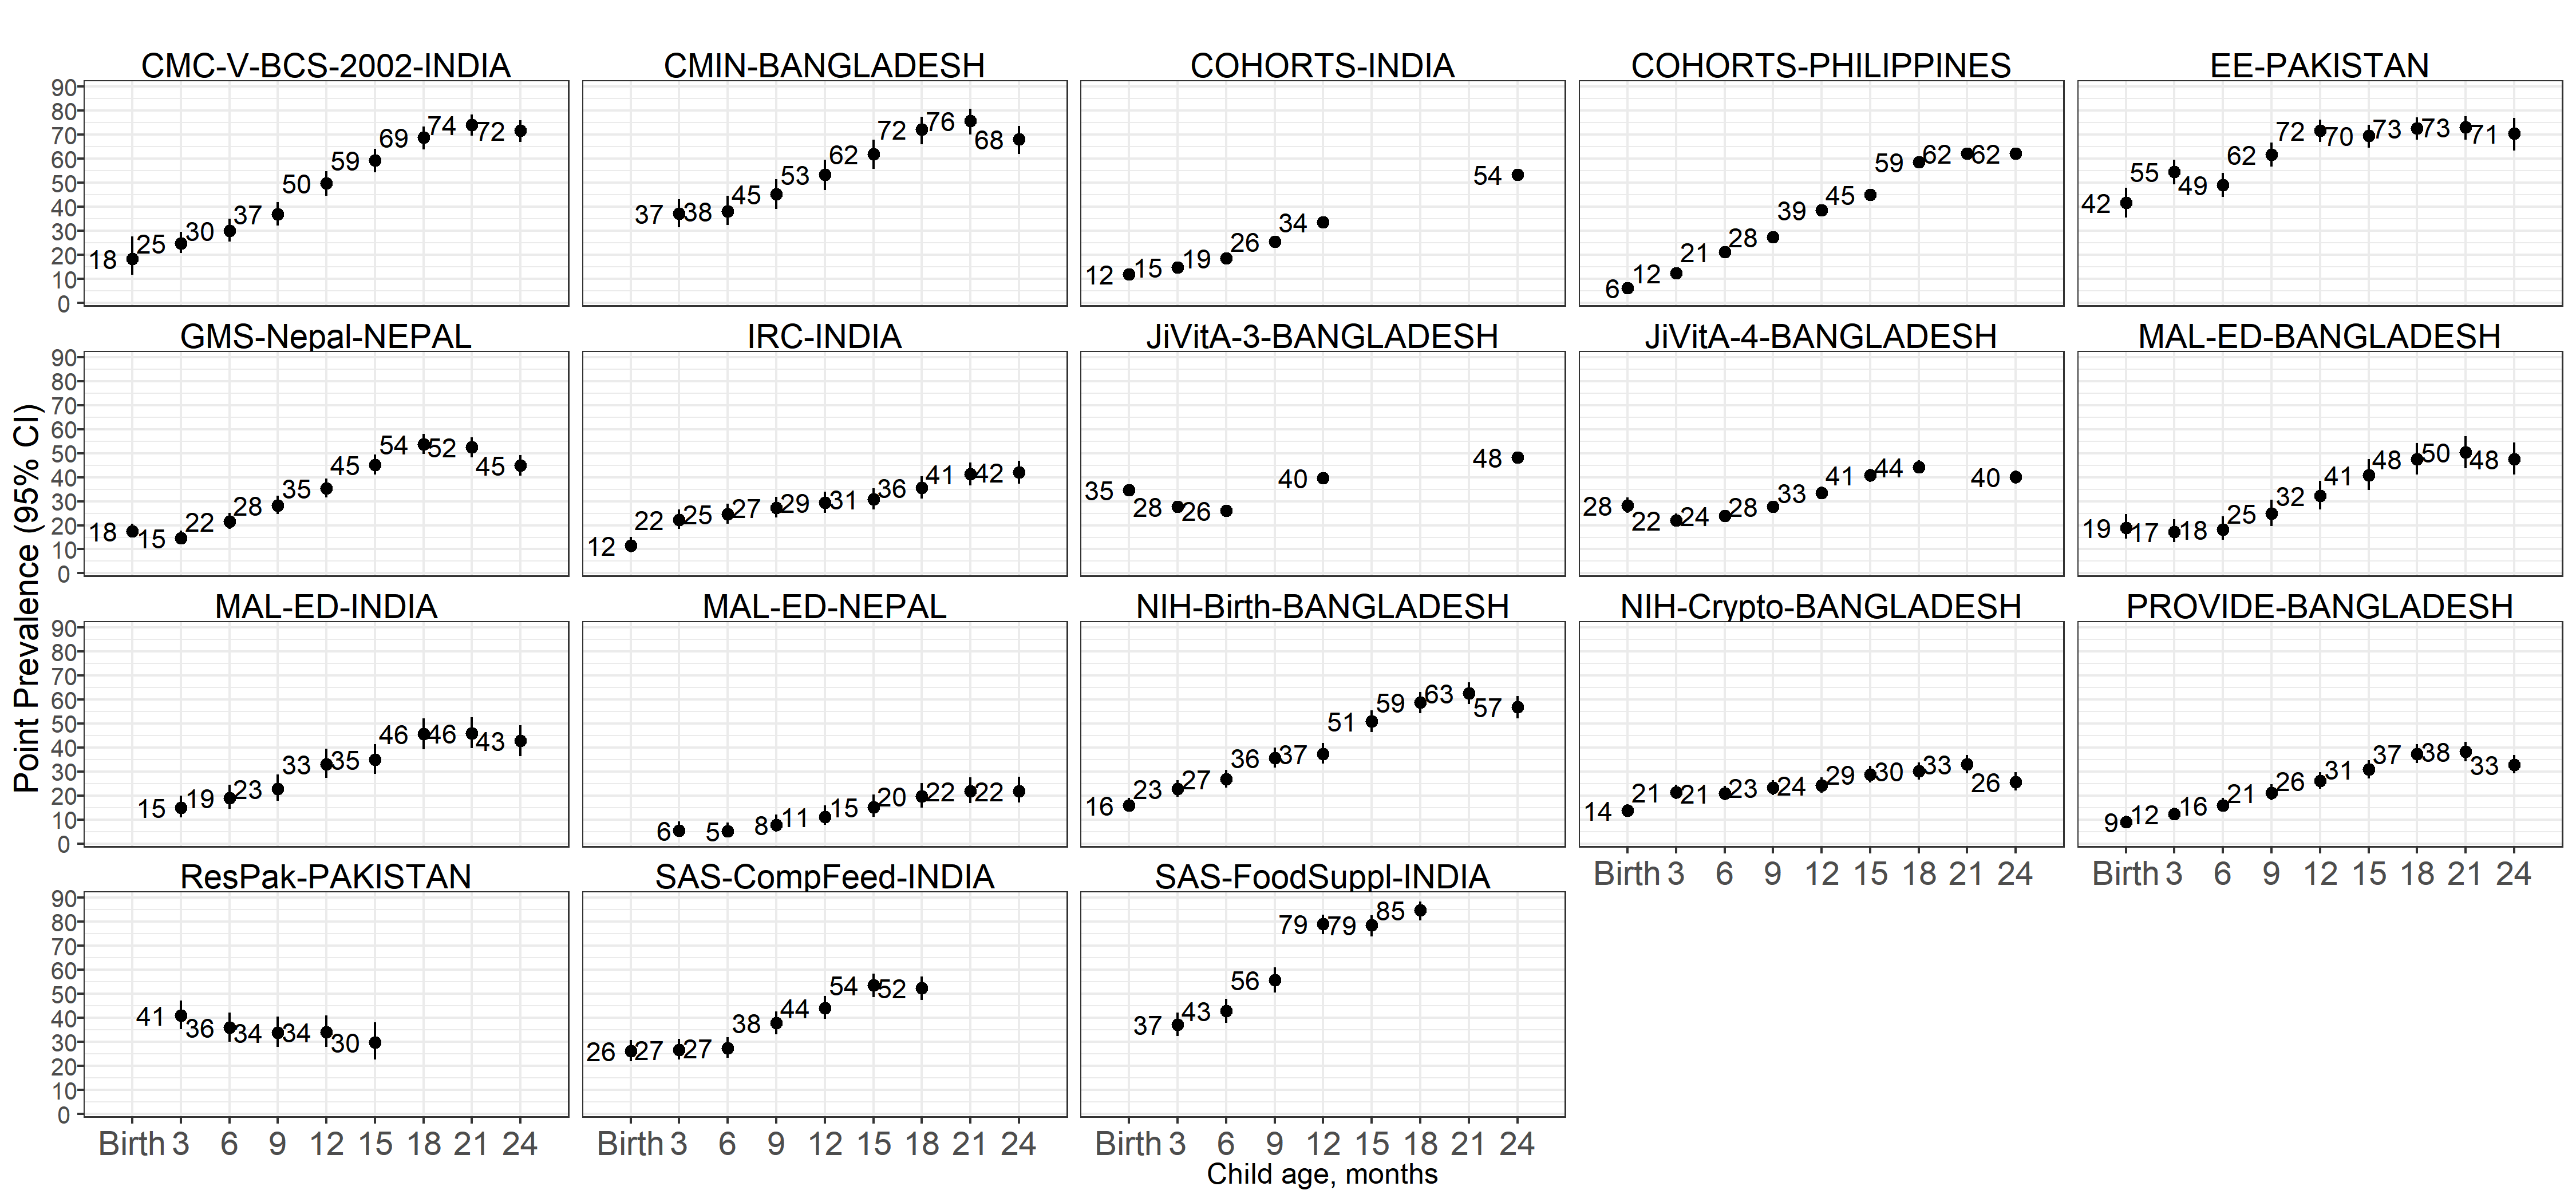
\includegraphics[width=62.5in]{figures//stunting/fig-stunt-2-prev-cohort-asia-allage-primary}

\hypertarget{age-specific-incidence}{%
\section{Age-specific incidence}\label{age-specific-incidence}}

\hypertarget{africa-2}{%
\subsection{Africa}\label{africa-2}}


\includegraphics[width=41.67in]{figures//stunting/fig-stunt-2-inc-cohort-africa-allage-primary}

\hypertarget{latin-america-2}{%
\subsection{Latin America}\label{latin-america-2}}

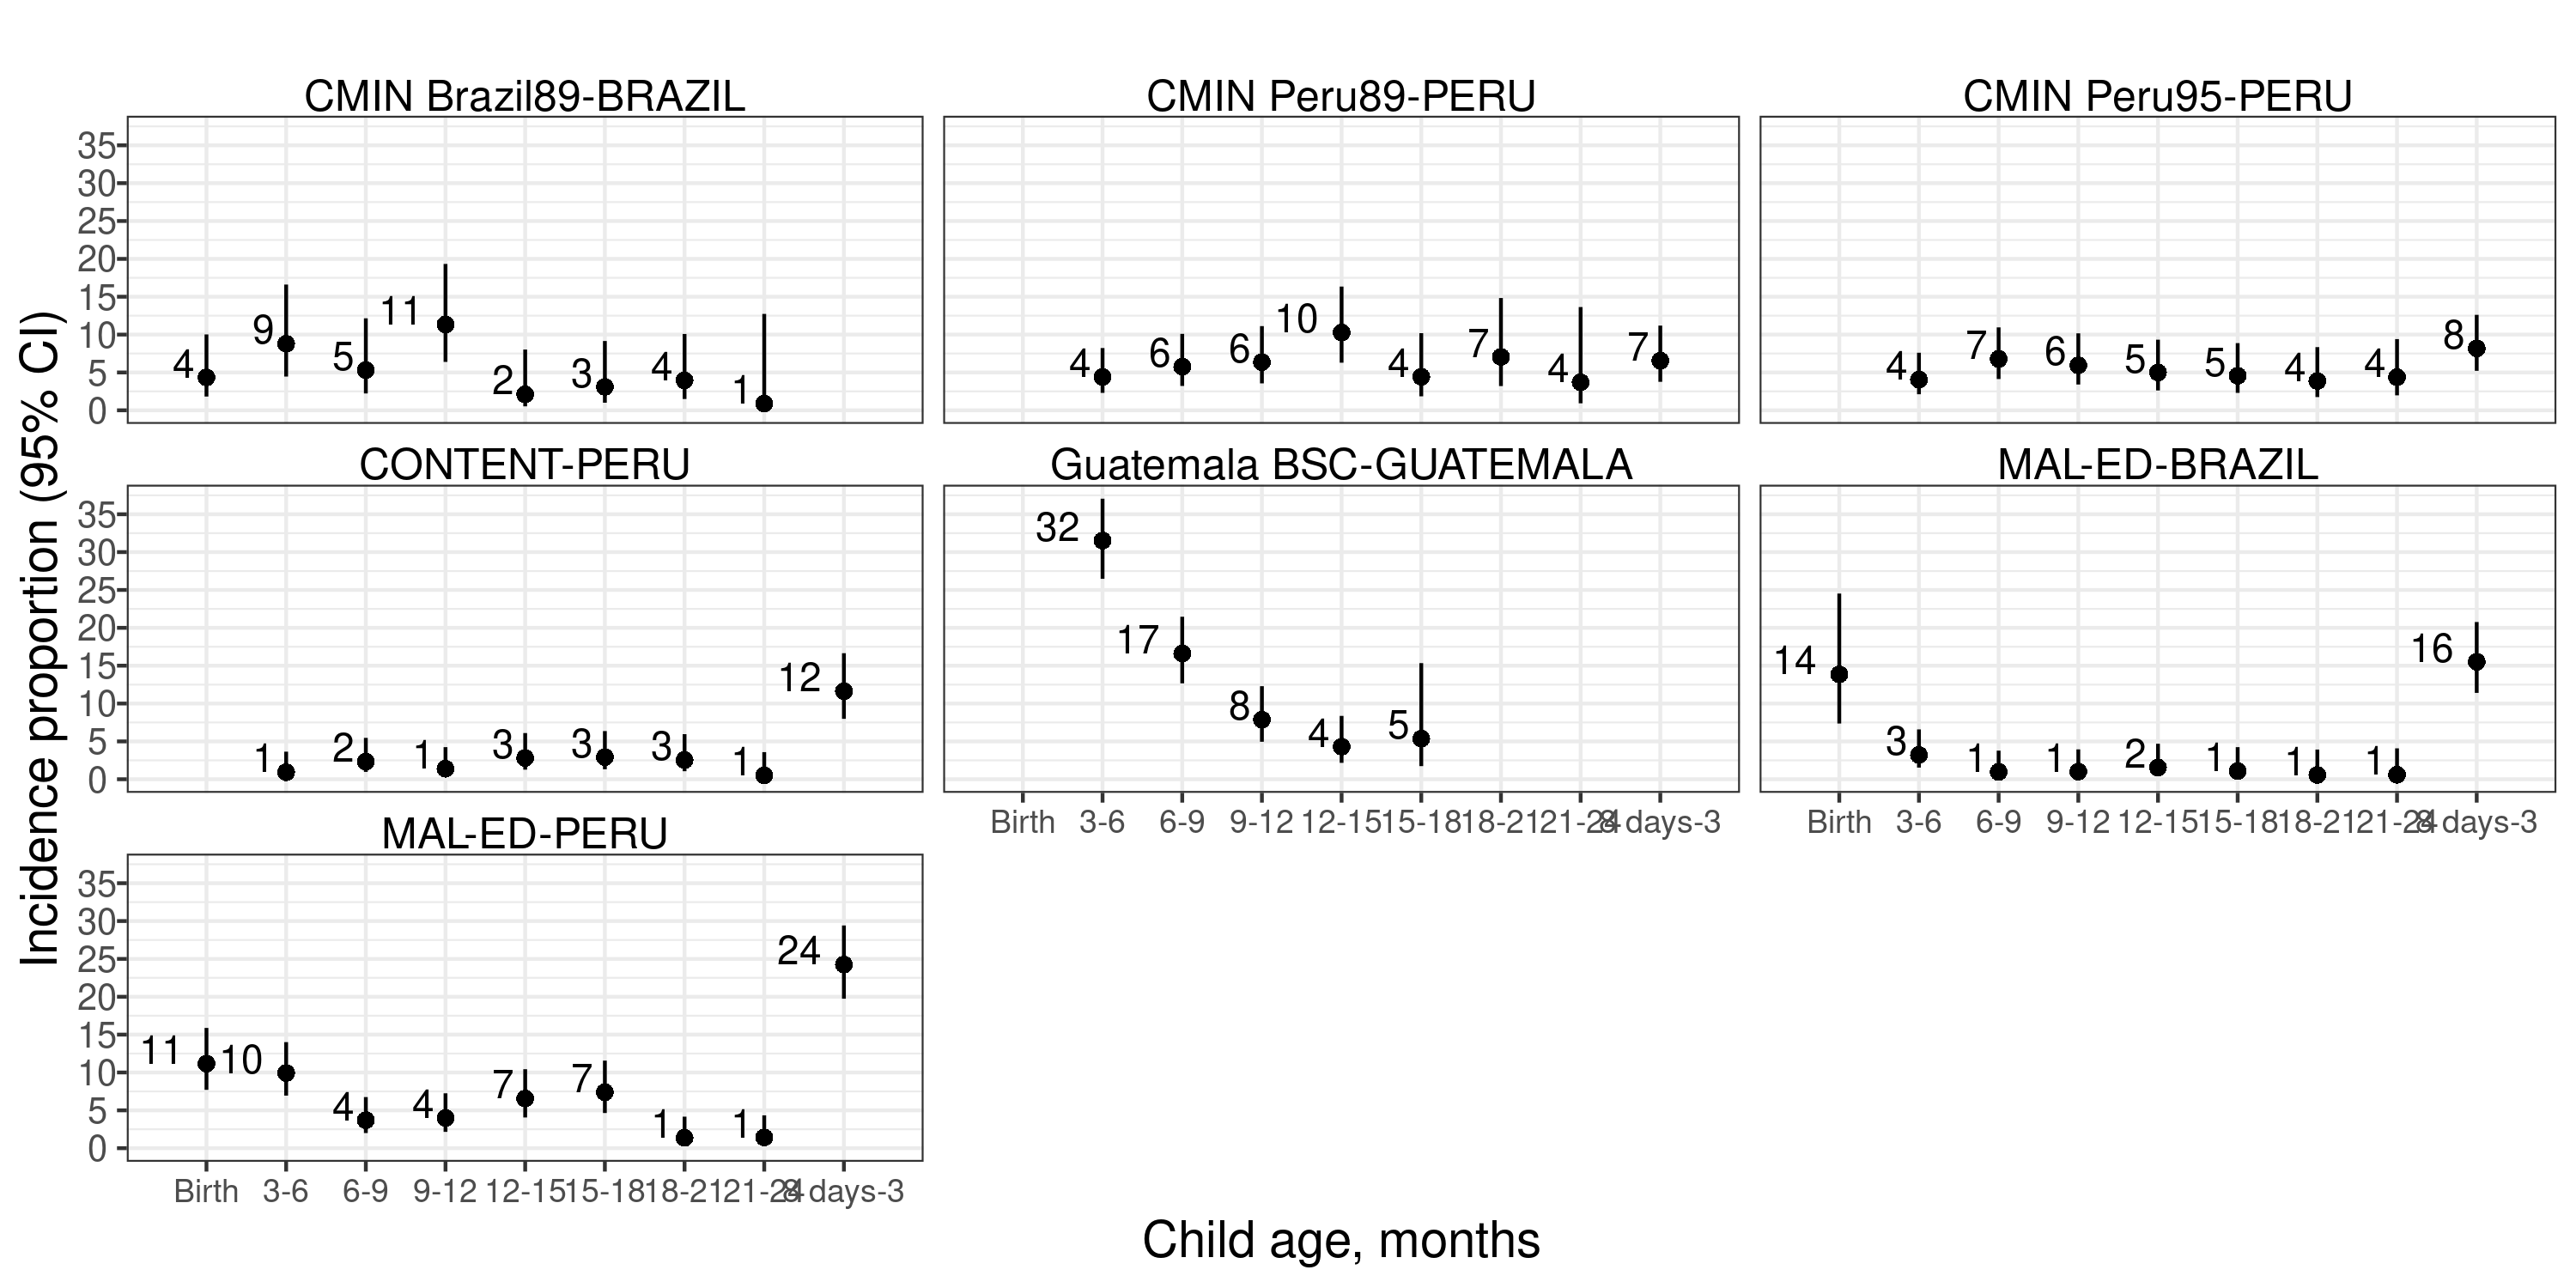
\includegraphics[width=41.67in]{figures//stunting/fig-stunt-2-inc-cohort-latamer-allage-primary}

\hypertarget{south-asia-2}{%
\subsection{South Asia}\label{south-asia-2}}

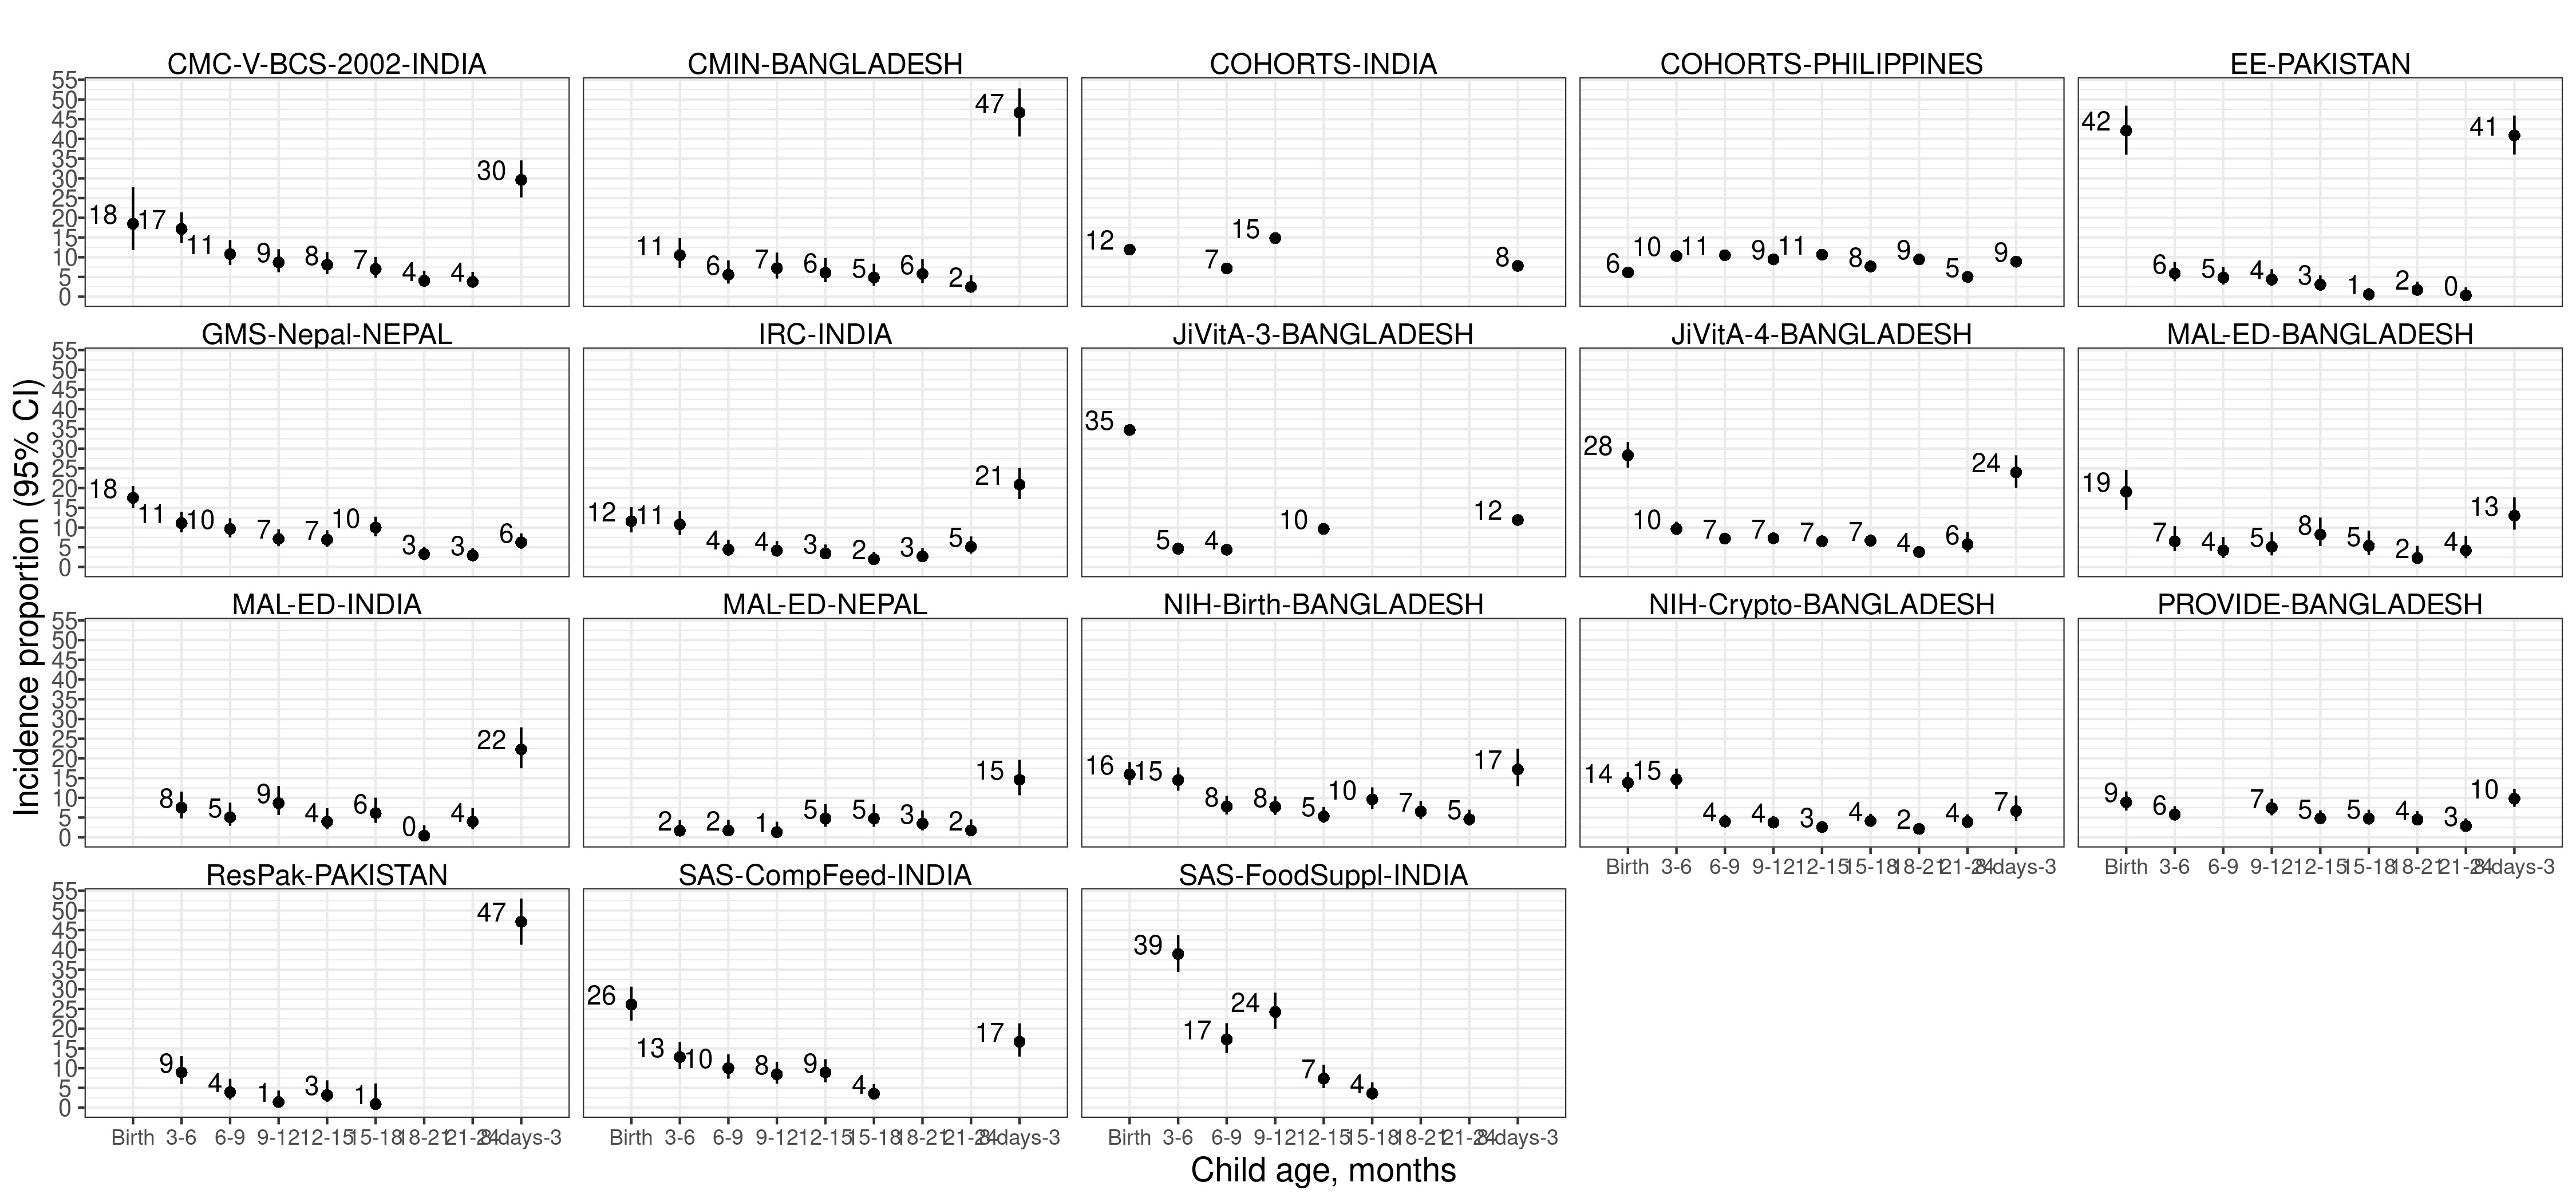
\includegraphics[width=62.5in]{figures//stunting/fig-stunt-2-inc-cohort-asia-allage-primary}

\hypertarget{length-velocity-by-age-and-sex}{%
\section{Length velocity by age and sex}\label{length-velocity-by-age-and-sex}}

\hypertarget{africa-3}{%
\subsection{Africa}\label{africa-3}}

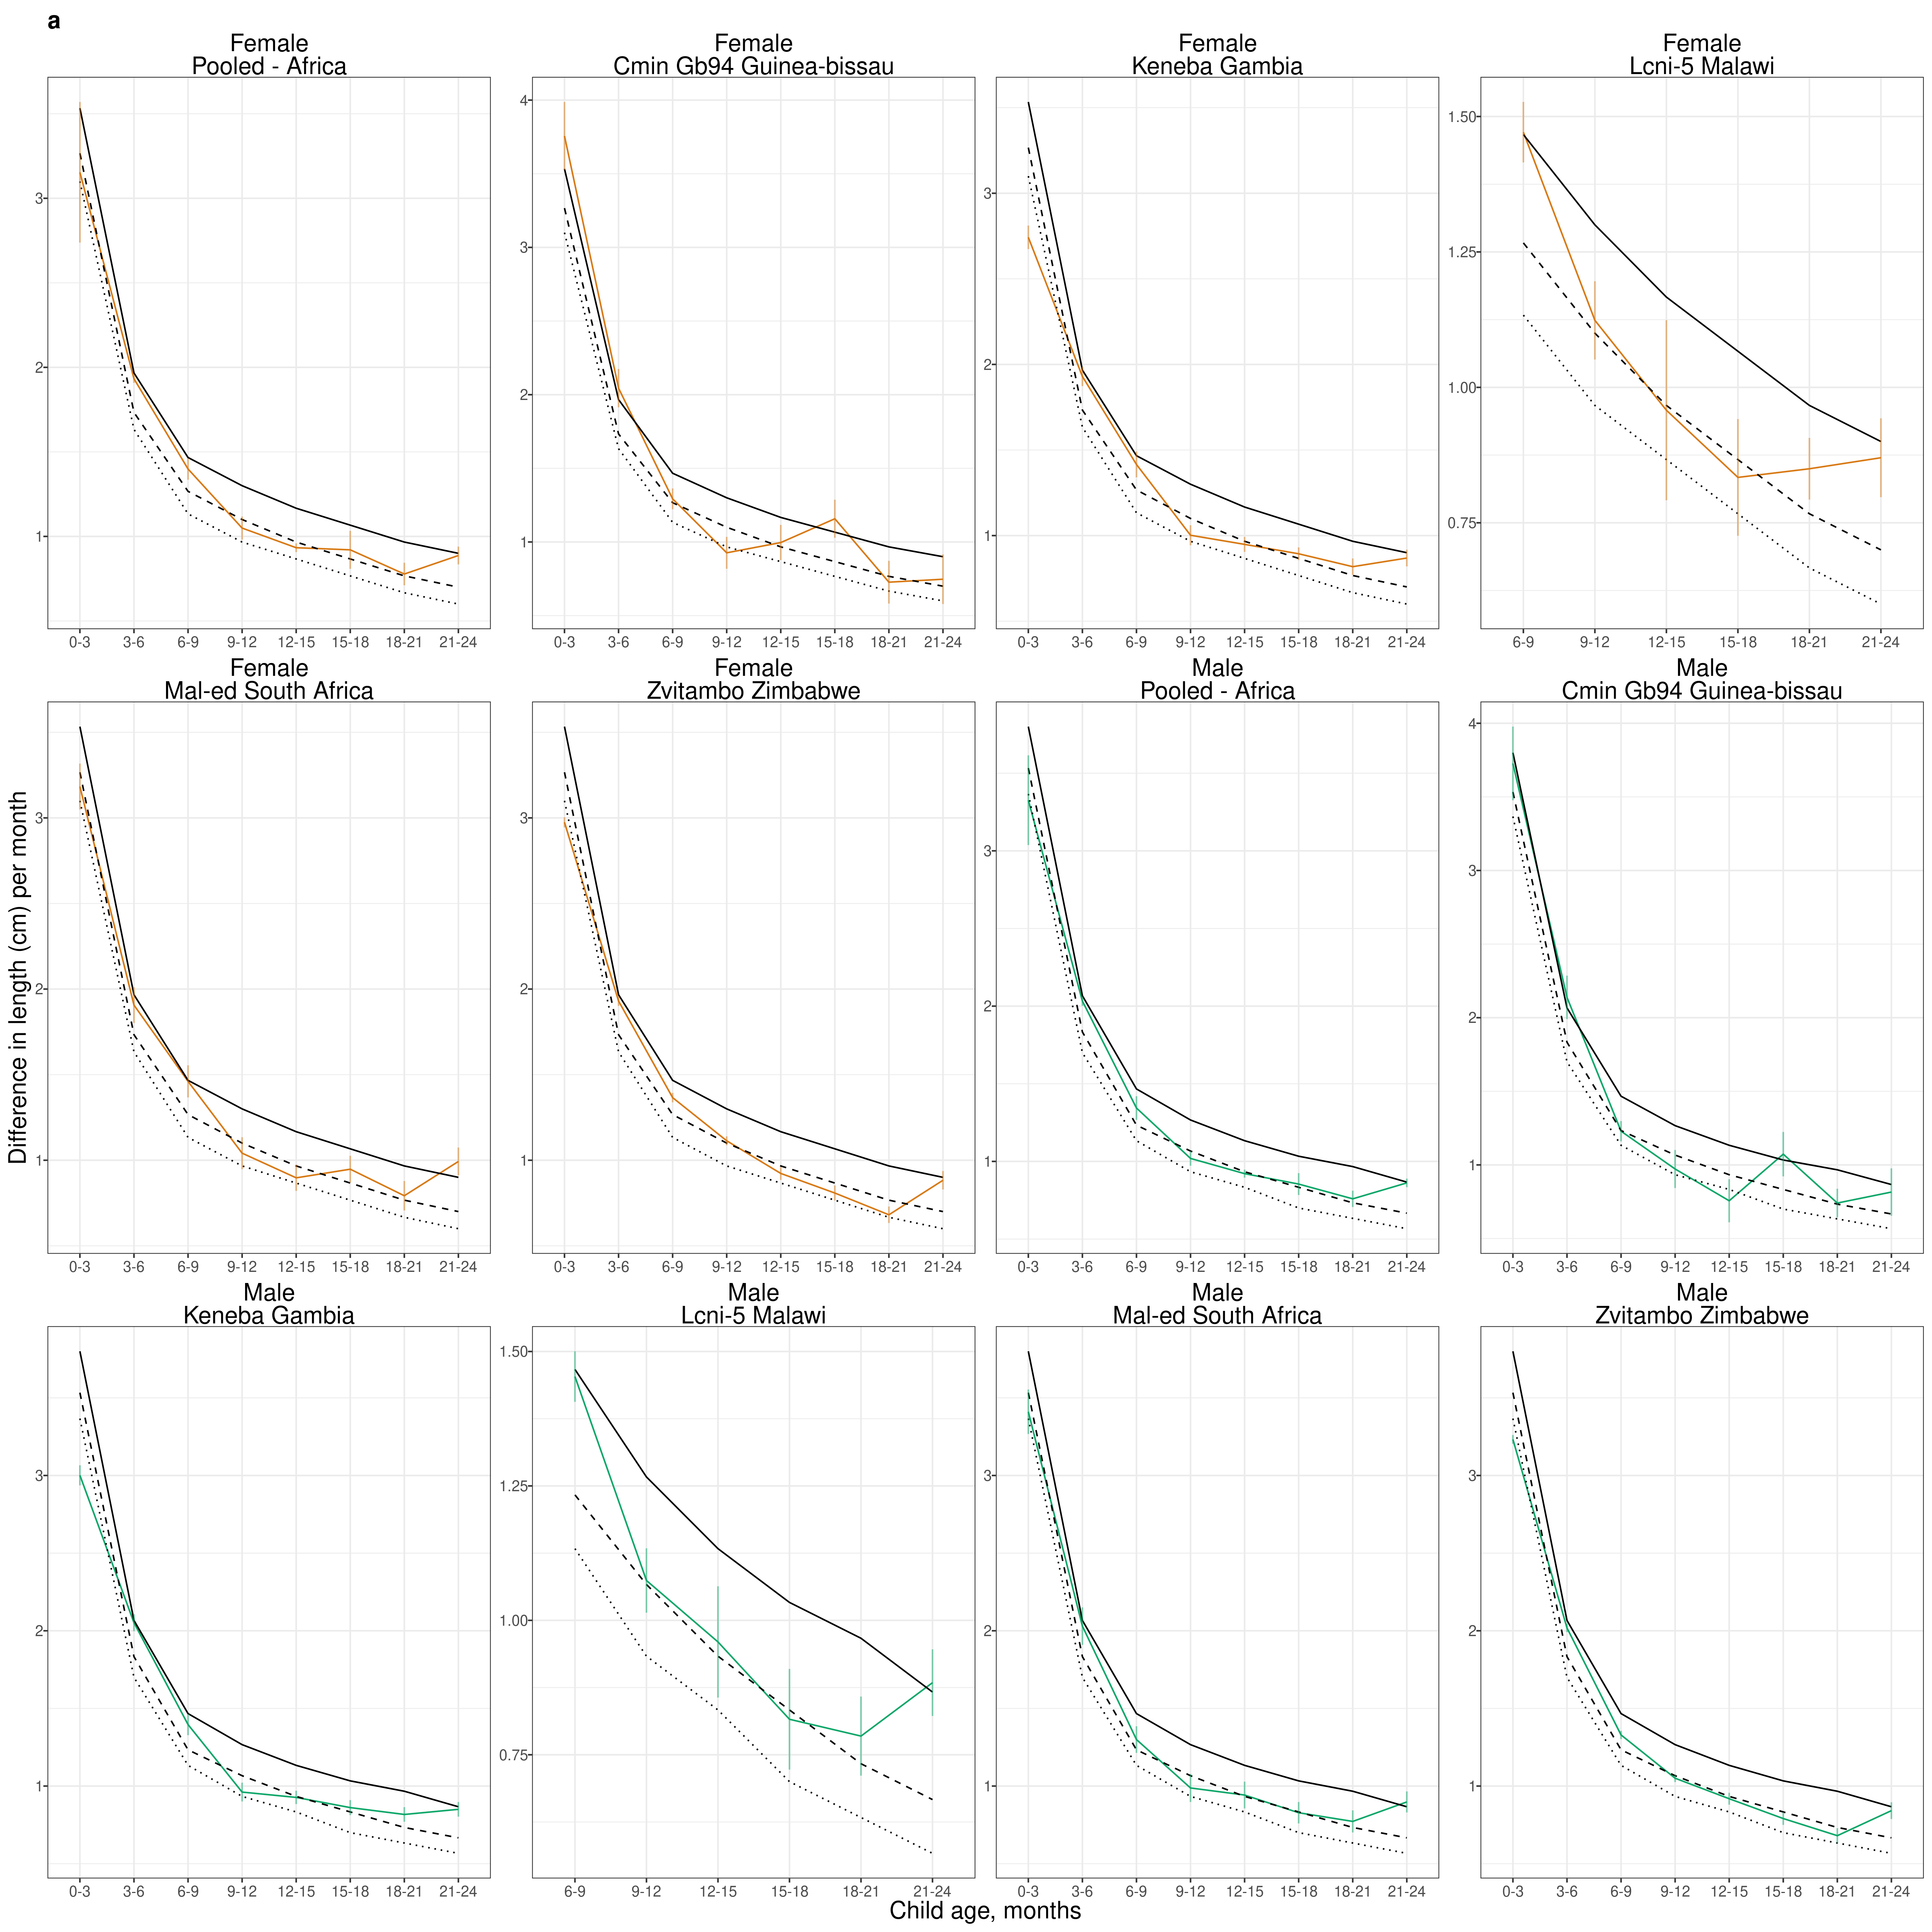
\includegraphics[width=75in]{figures//stunting/fig-length-2-length_vel-cohort-africa-allage-primary}

\hypertarget{latin-america-3}{%
\subsection{Latin America}\label{latin-america-3}}

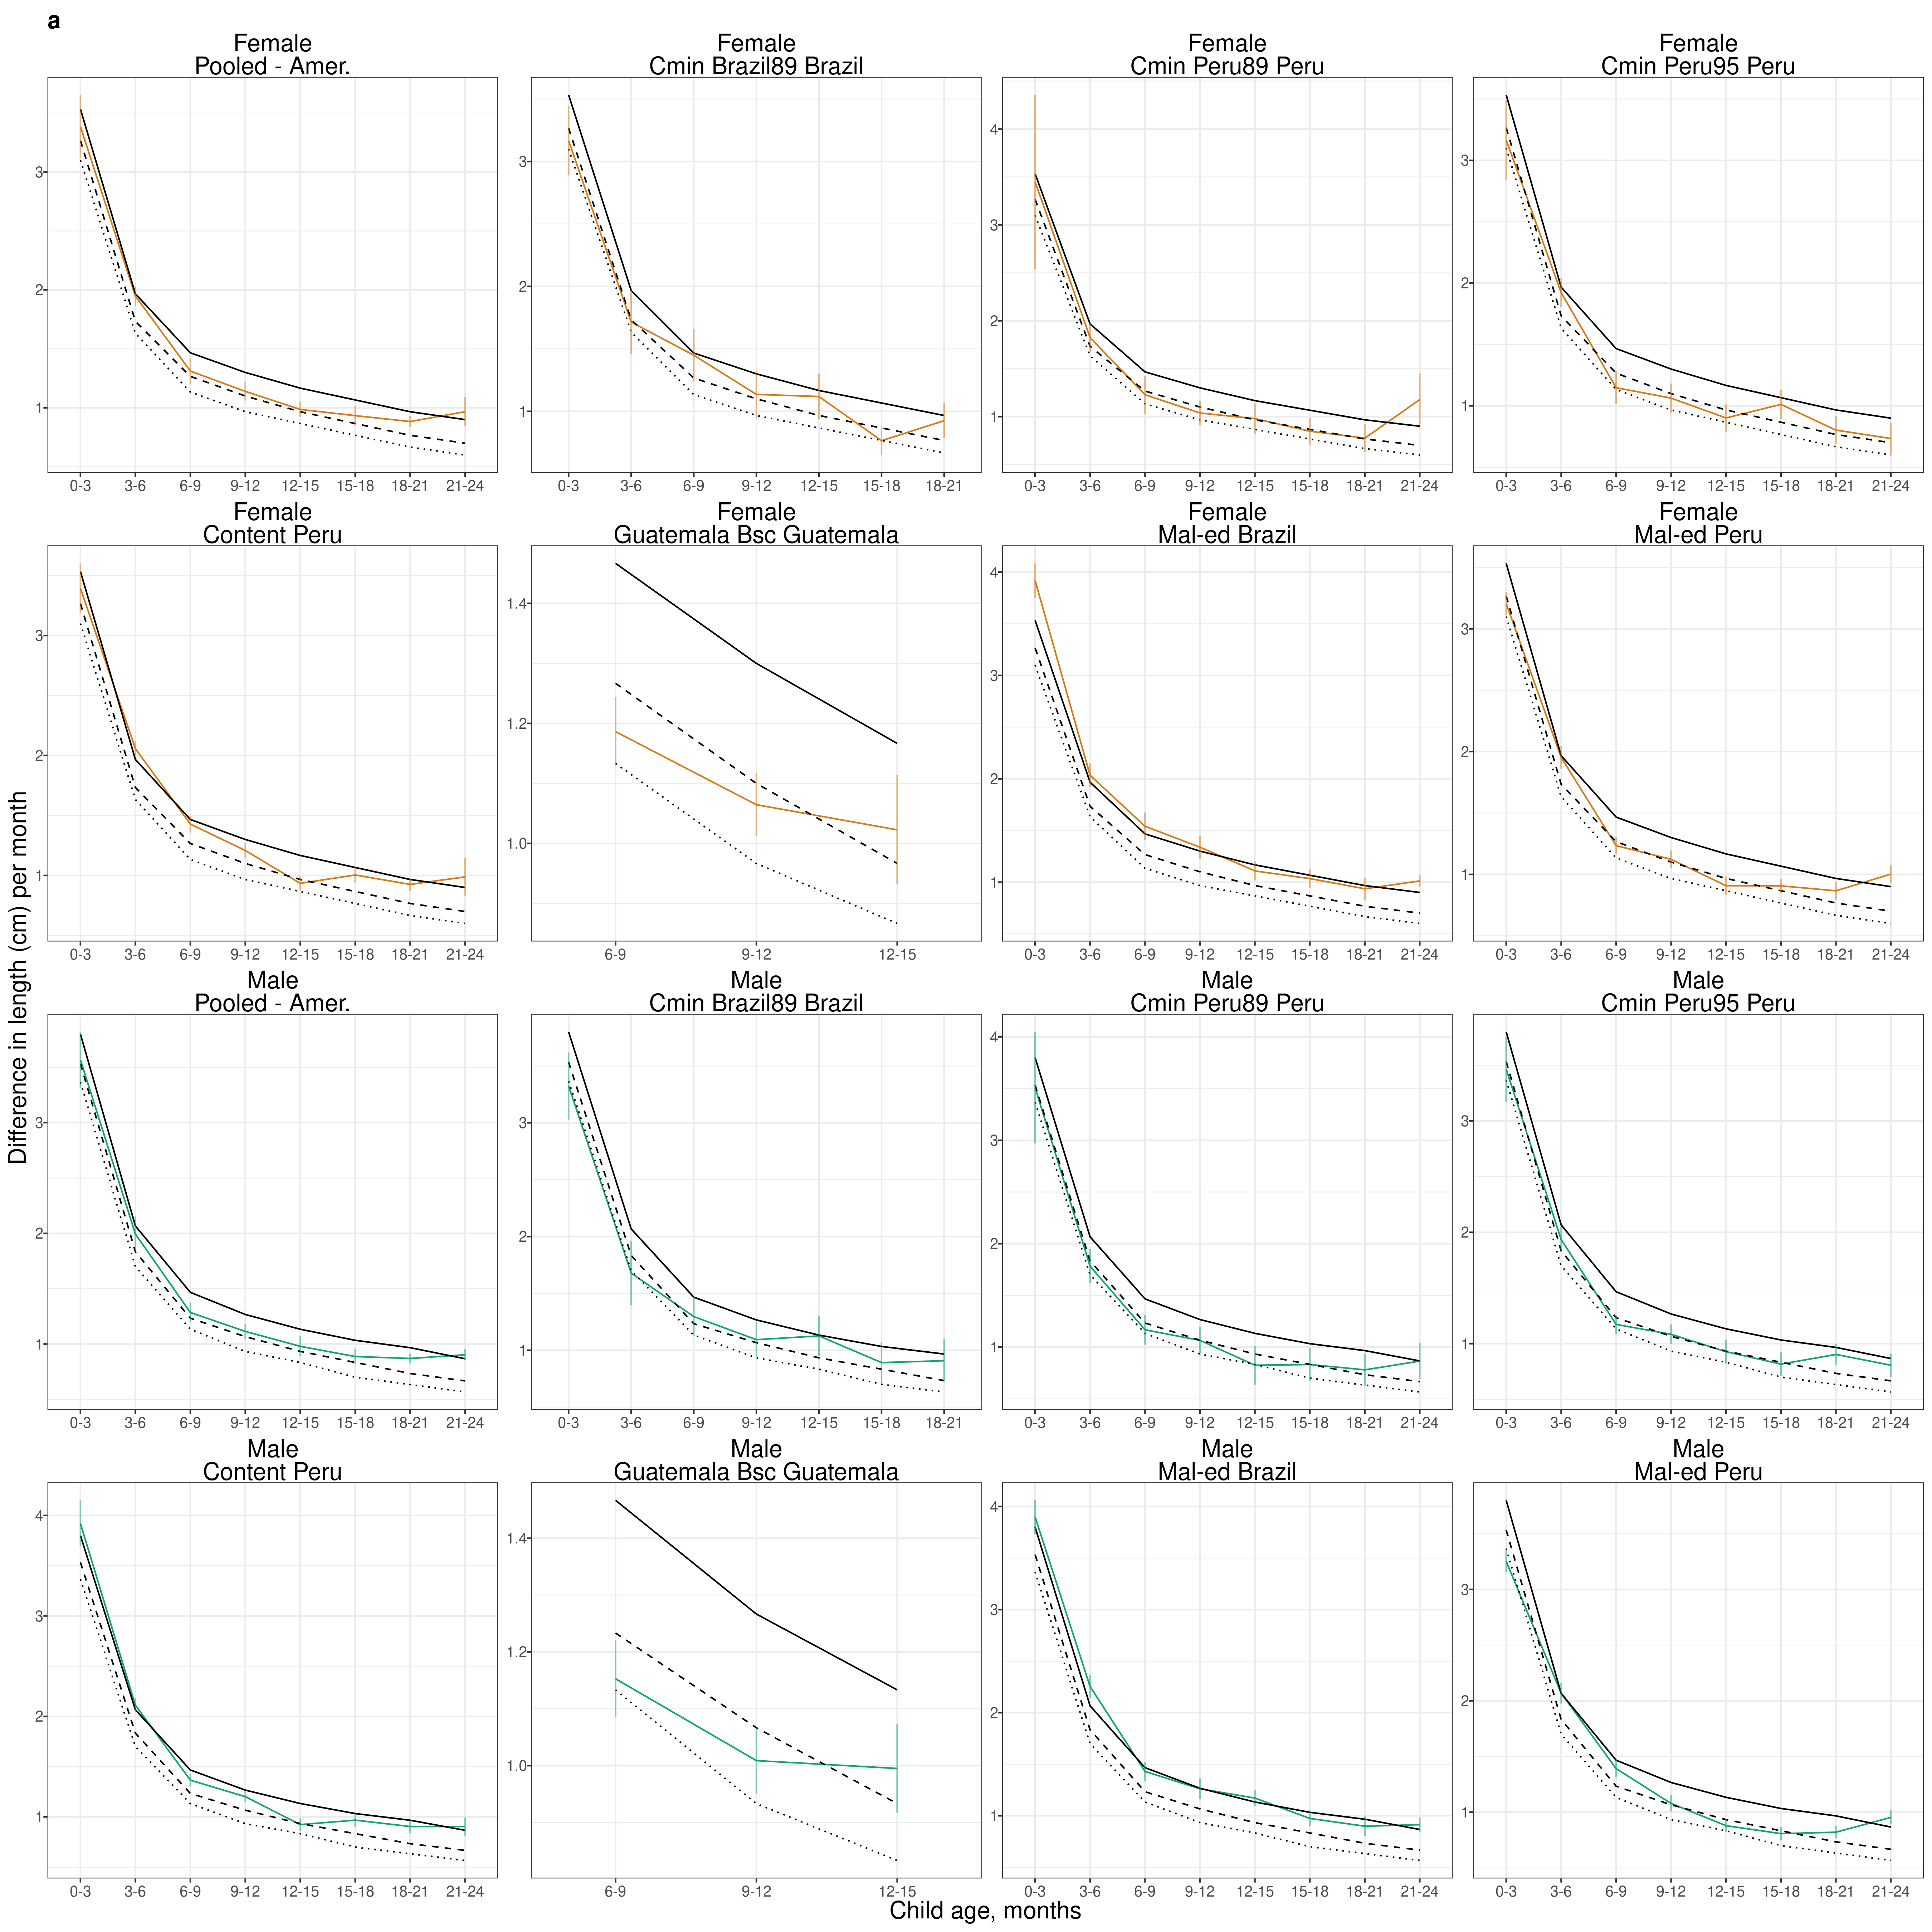
\includegraphics[width=75in]{figures//stunting/fig-length-2-length_vel-cohort-latamer-allage-primary}

\hypertarget{south-asia-3}{%
\subsection{South Asia}\label{south-asia-3}}

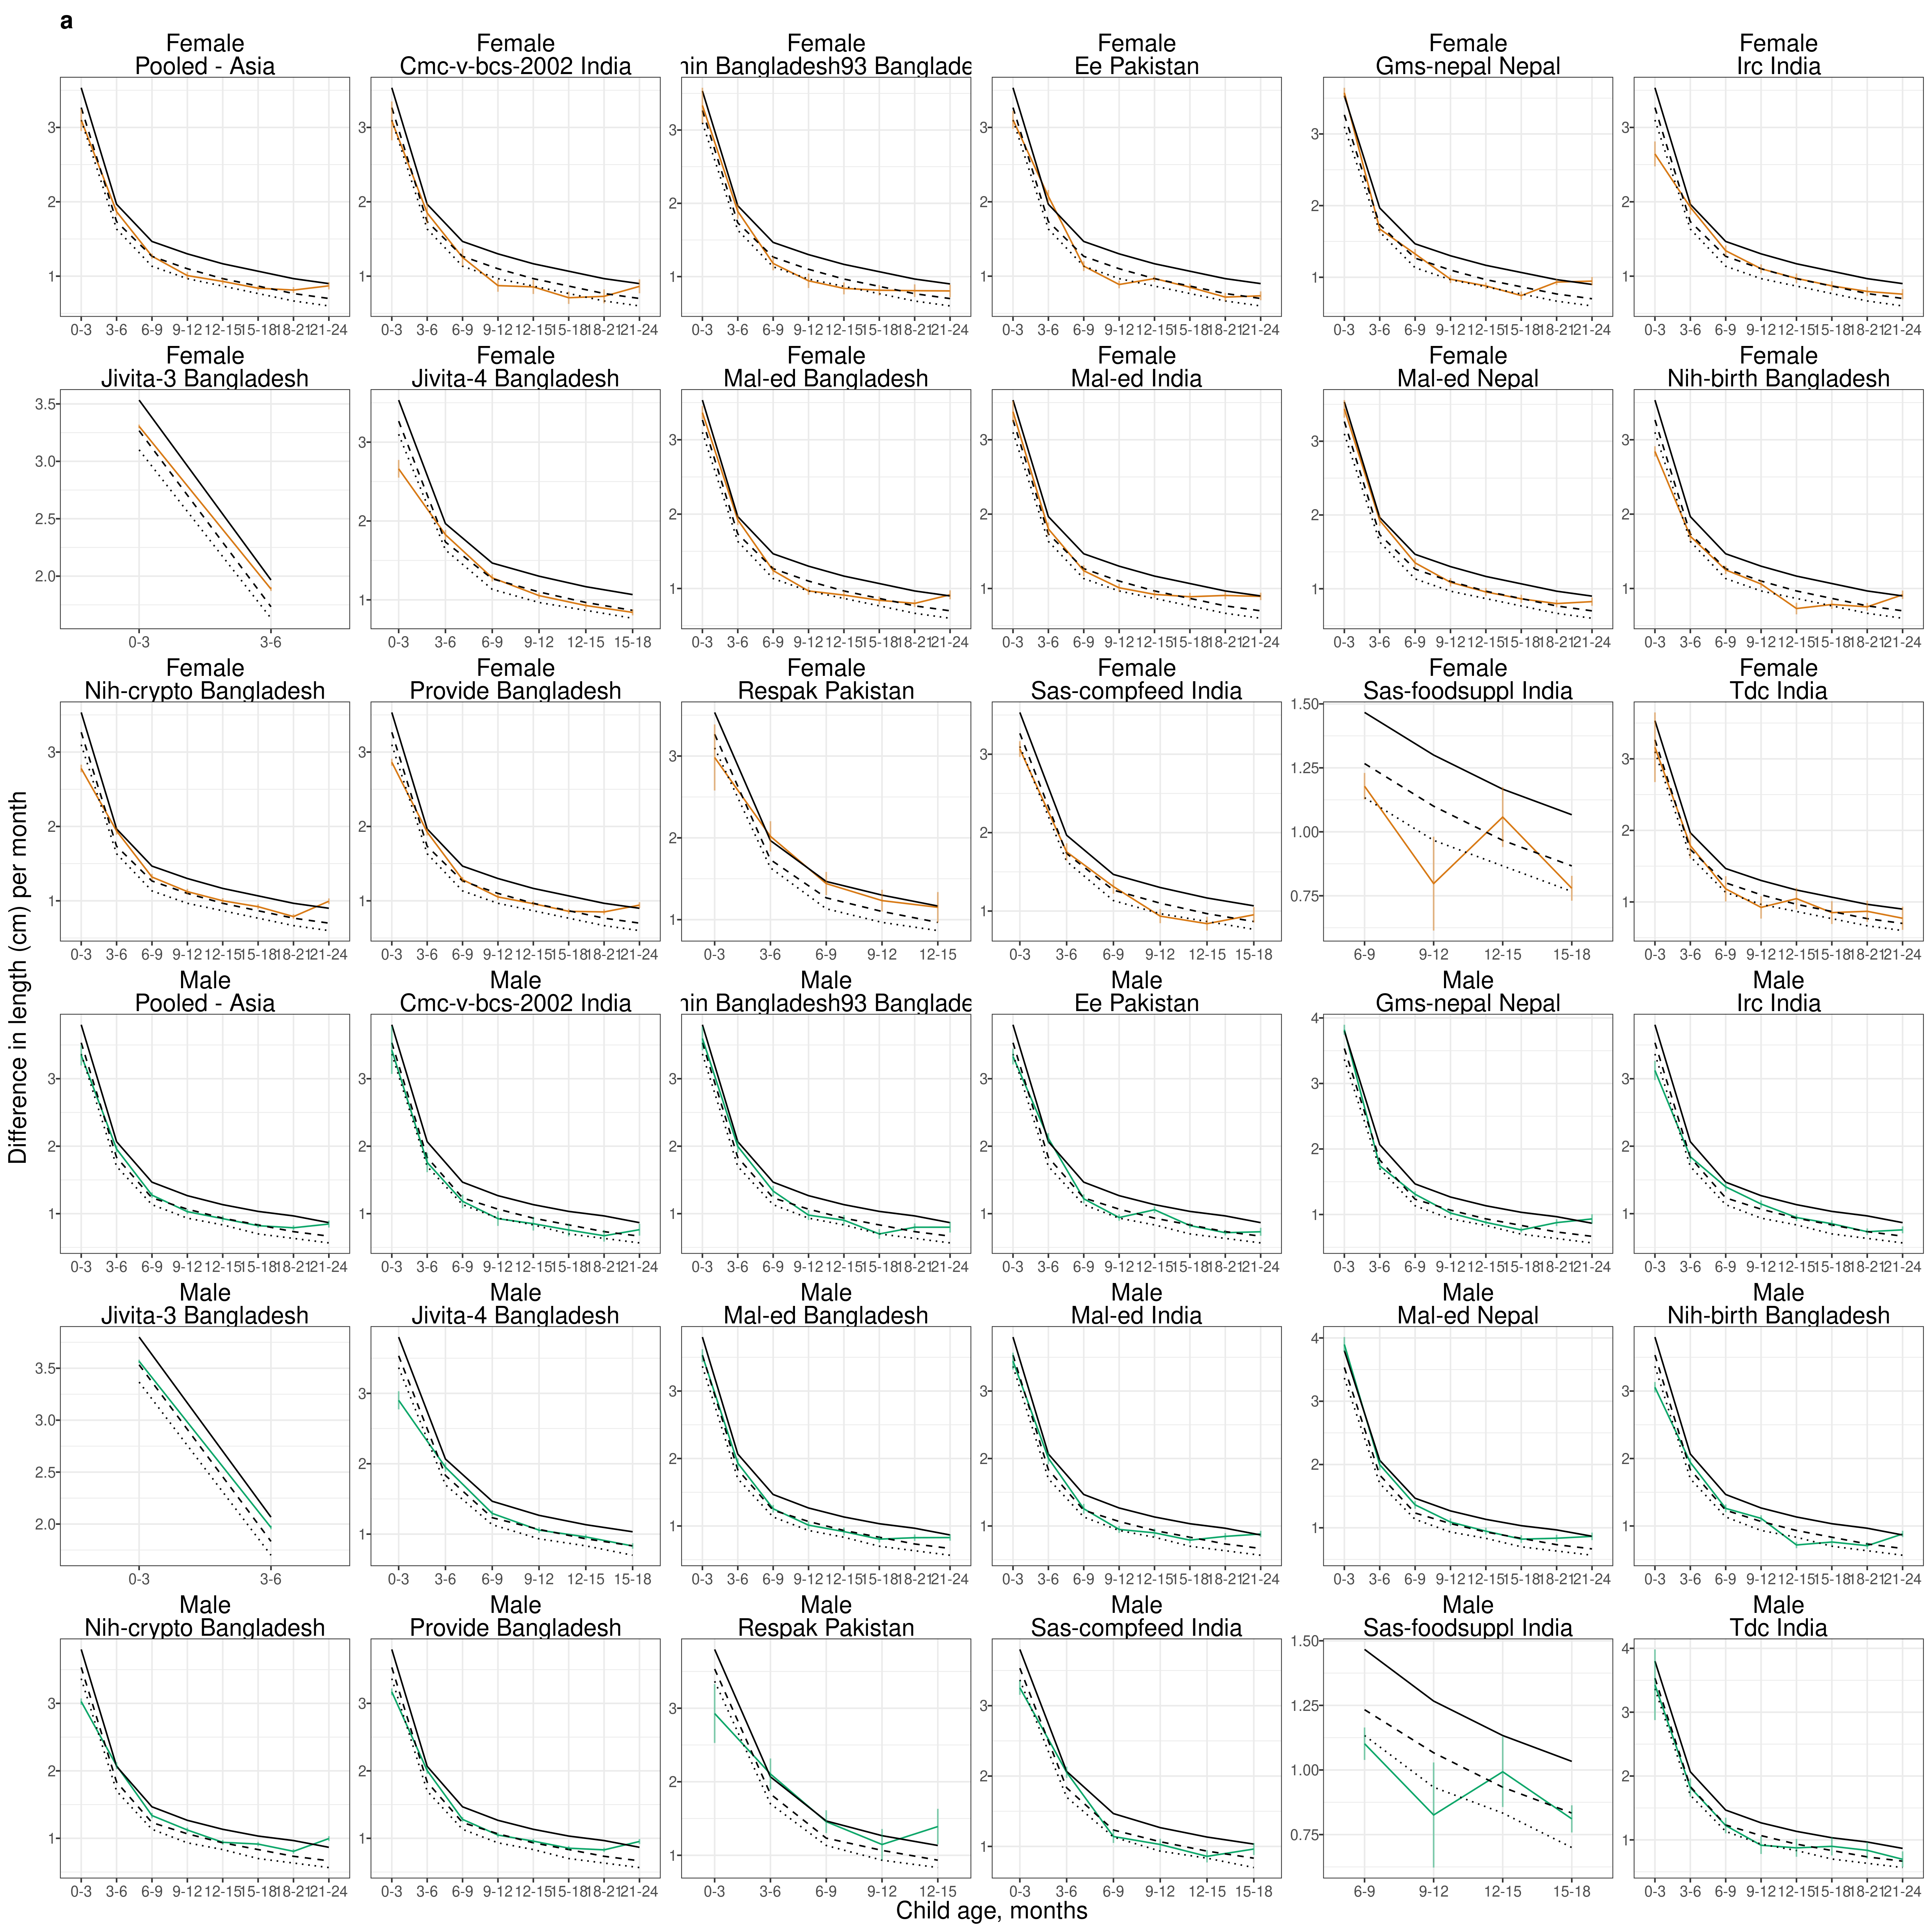
\includegraphics[width=75in]{figures//stunting/fig-length-2-length_vel-cohort-asia-allage-primary}

\hypertarget{laz-velocity-by-age-and-sex}{%
\section{LAZ velocity by age and sex}\label{laz-velocity-by-age-and-sex}}

\hypertarget{africa-4}{%
\subsection{Africa}\label{africa-4}}

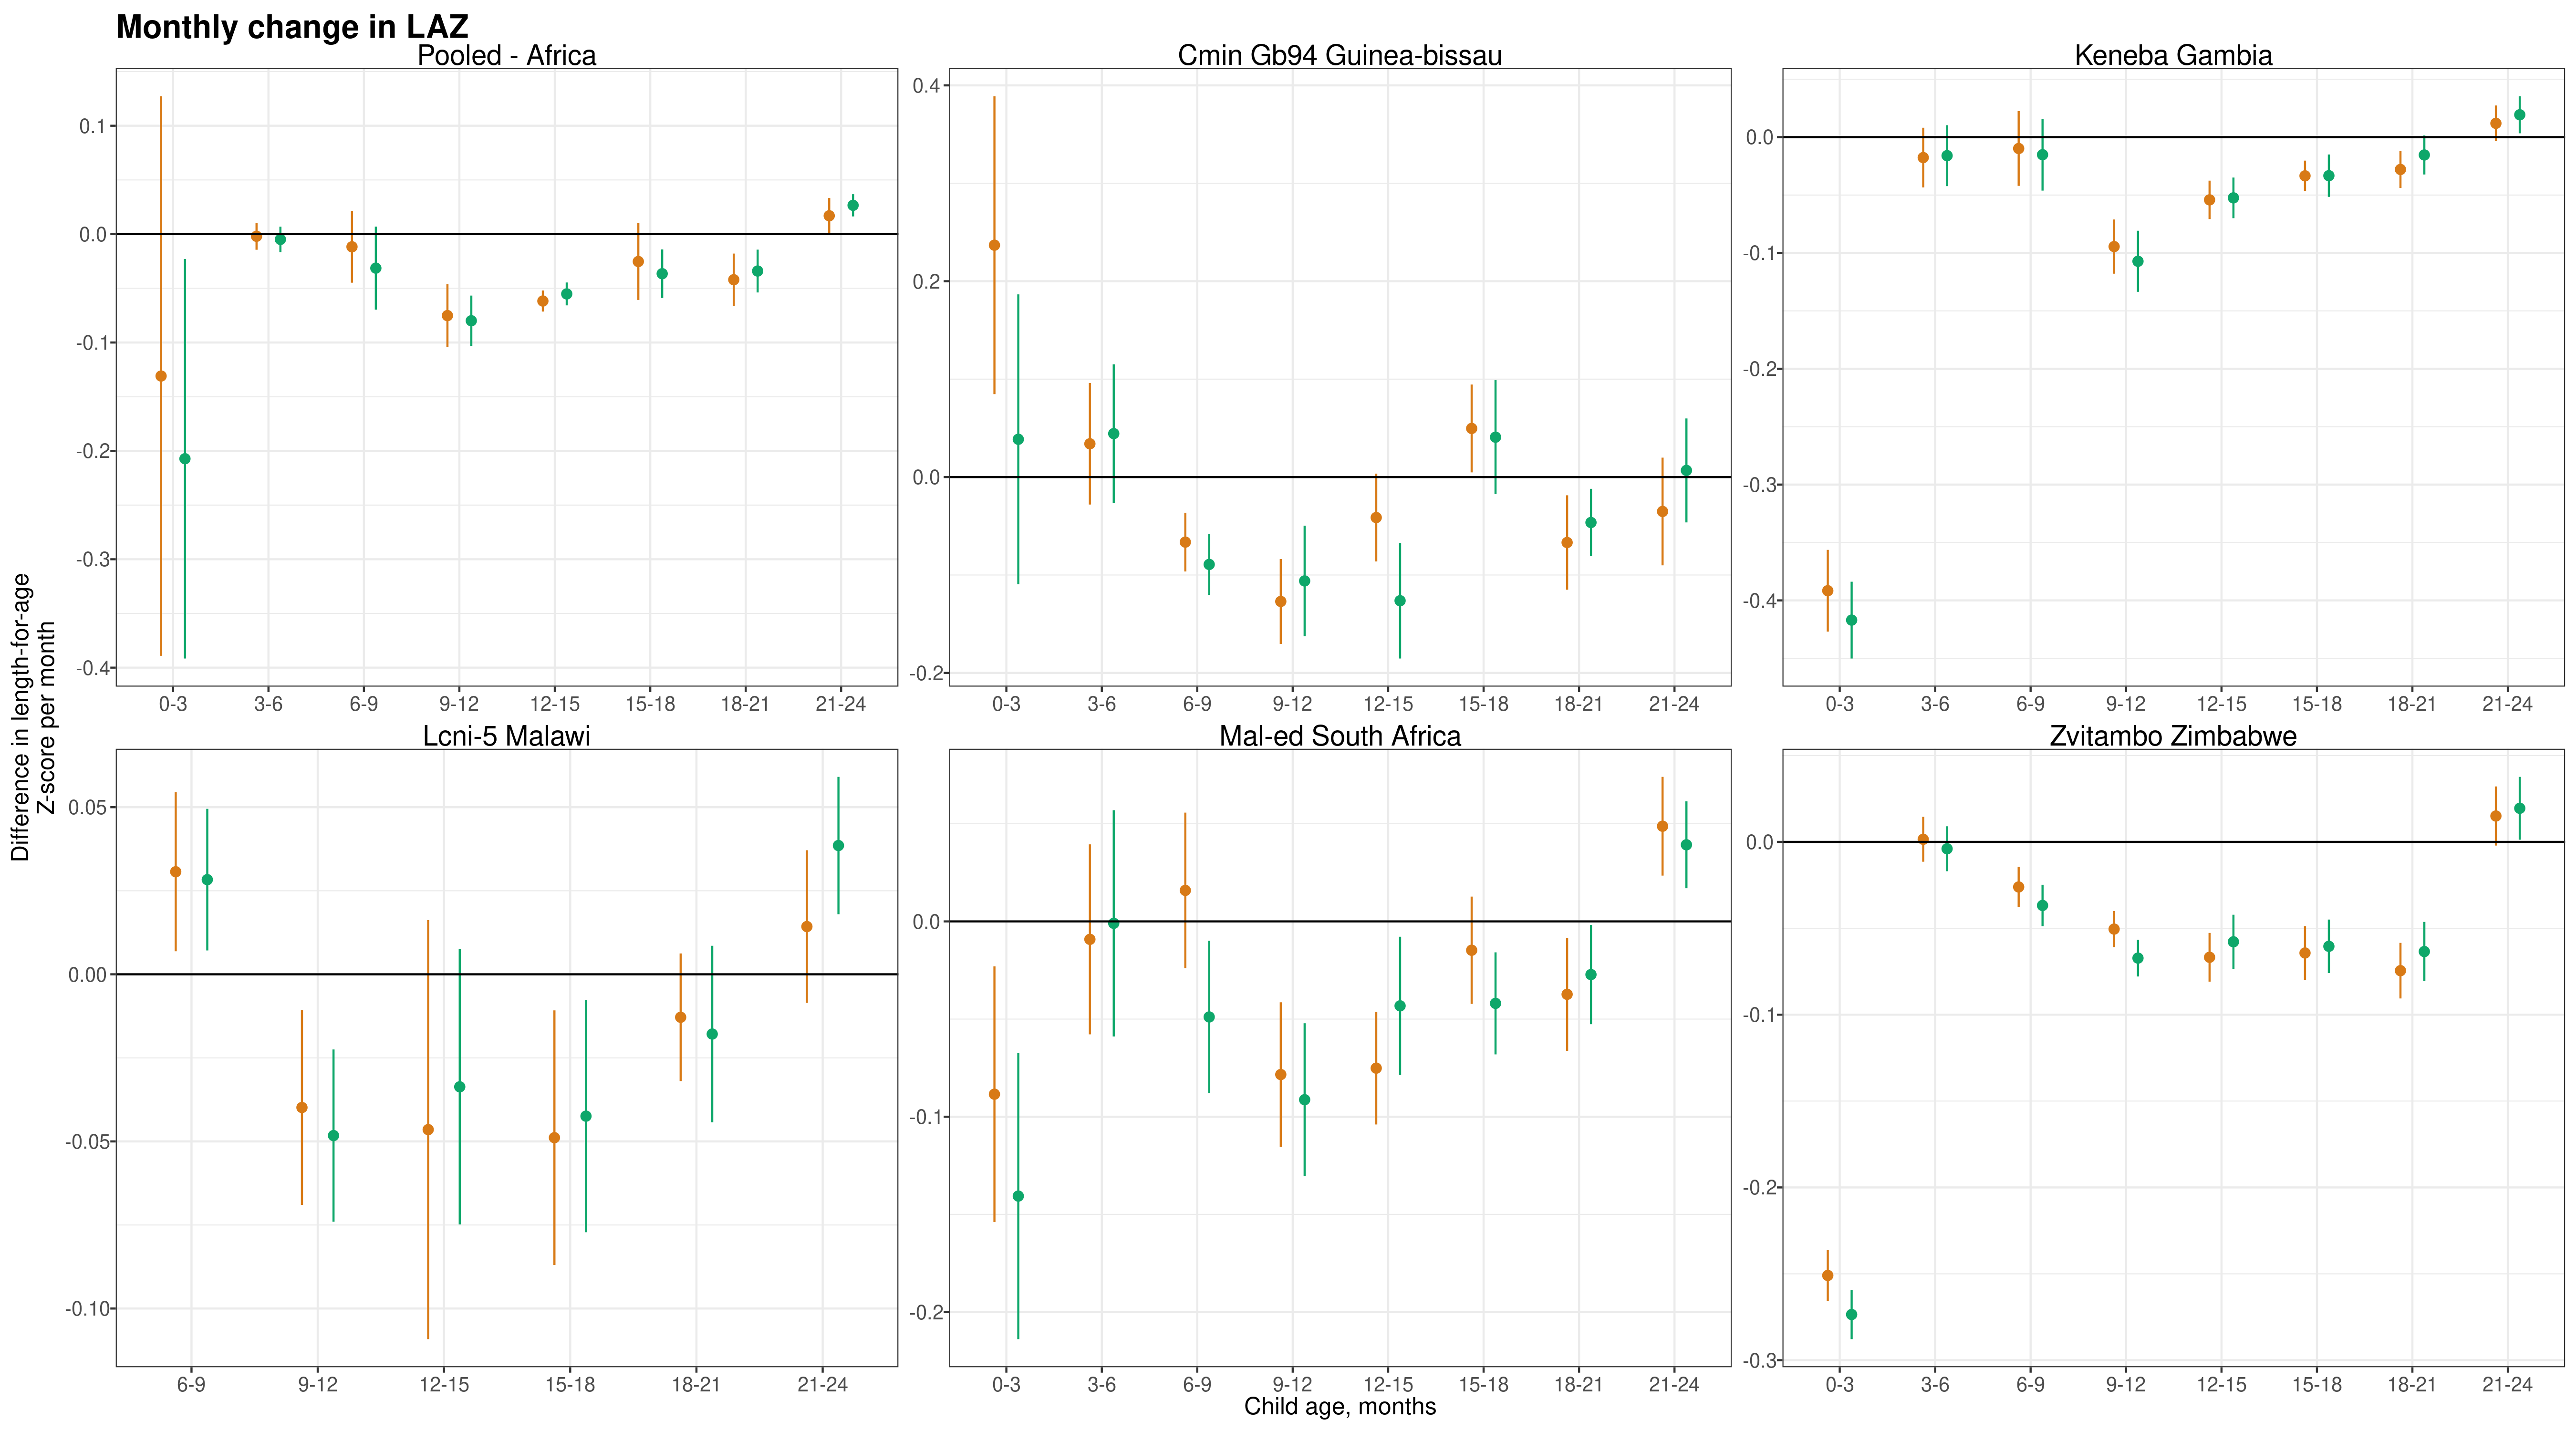
\includegraphics[width=75in]{figures//stunting/fig-laz-2-laz_vel-cohort-africa-allage-primary}

\hypertarget{latin-america-4}{%
\subsection{Latin America}\label{latin-america-4}}

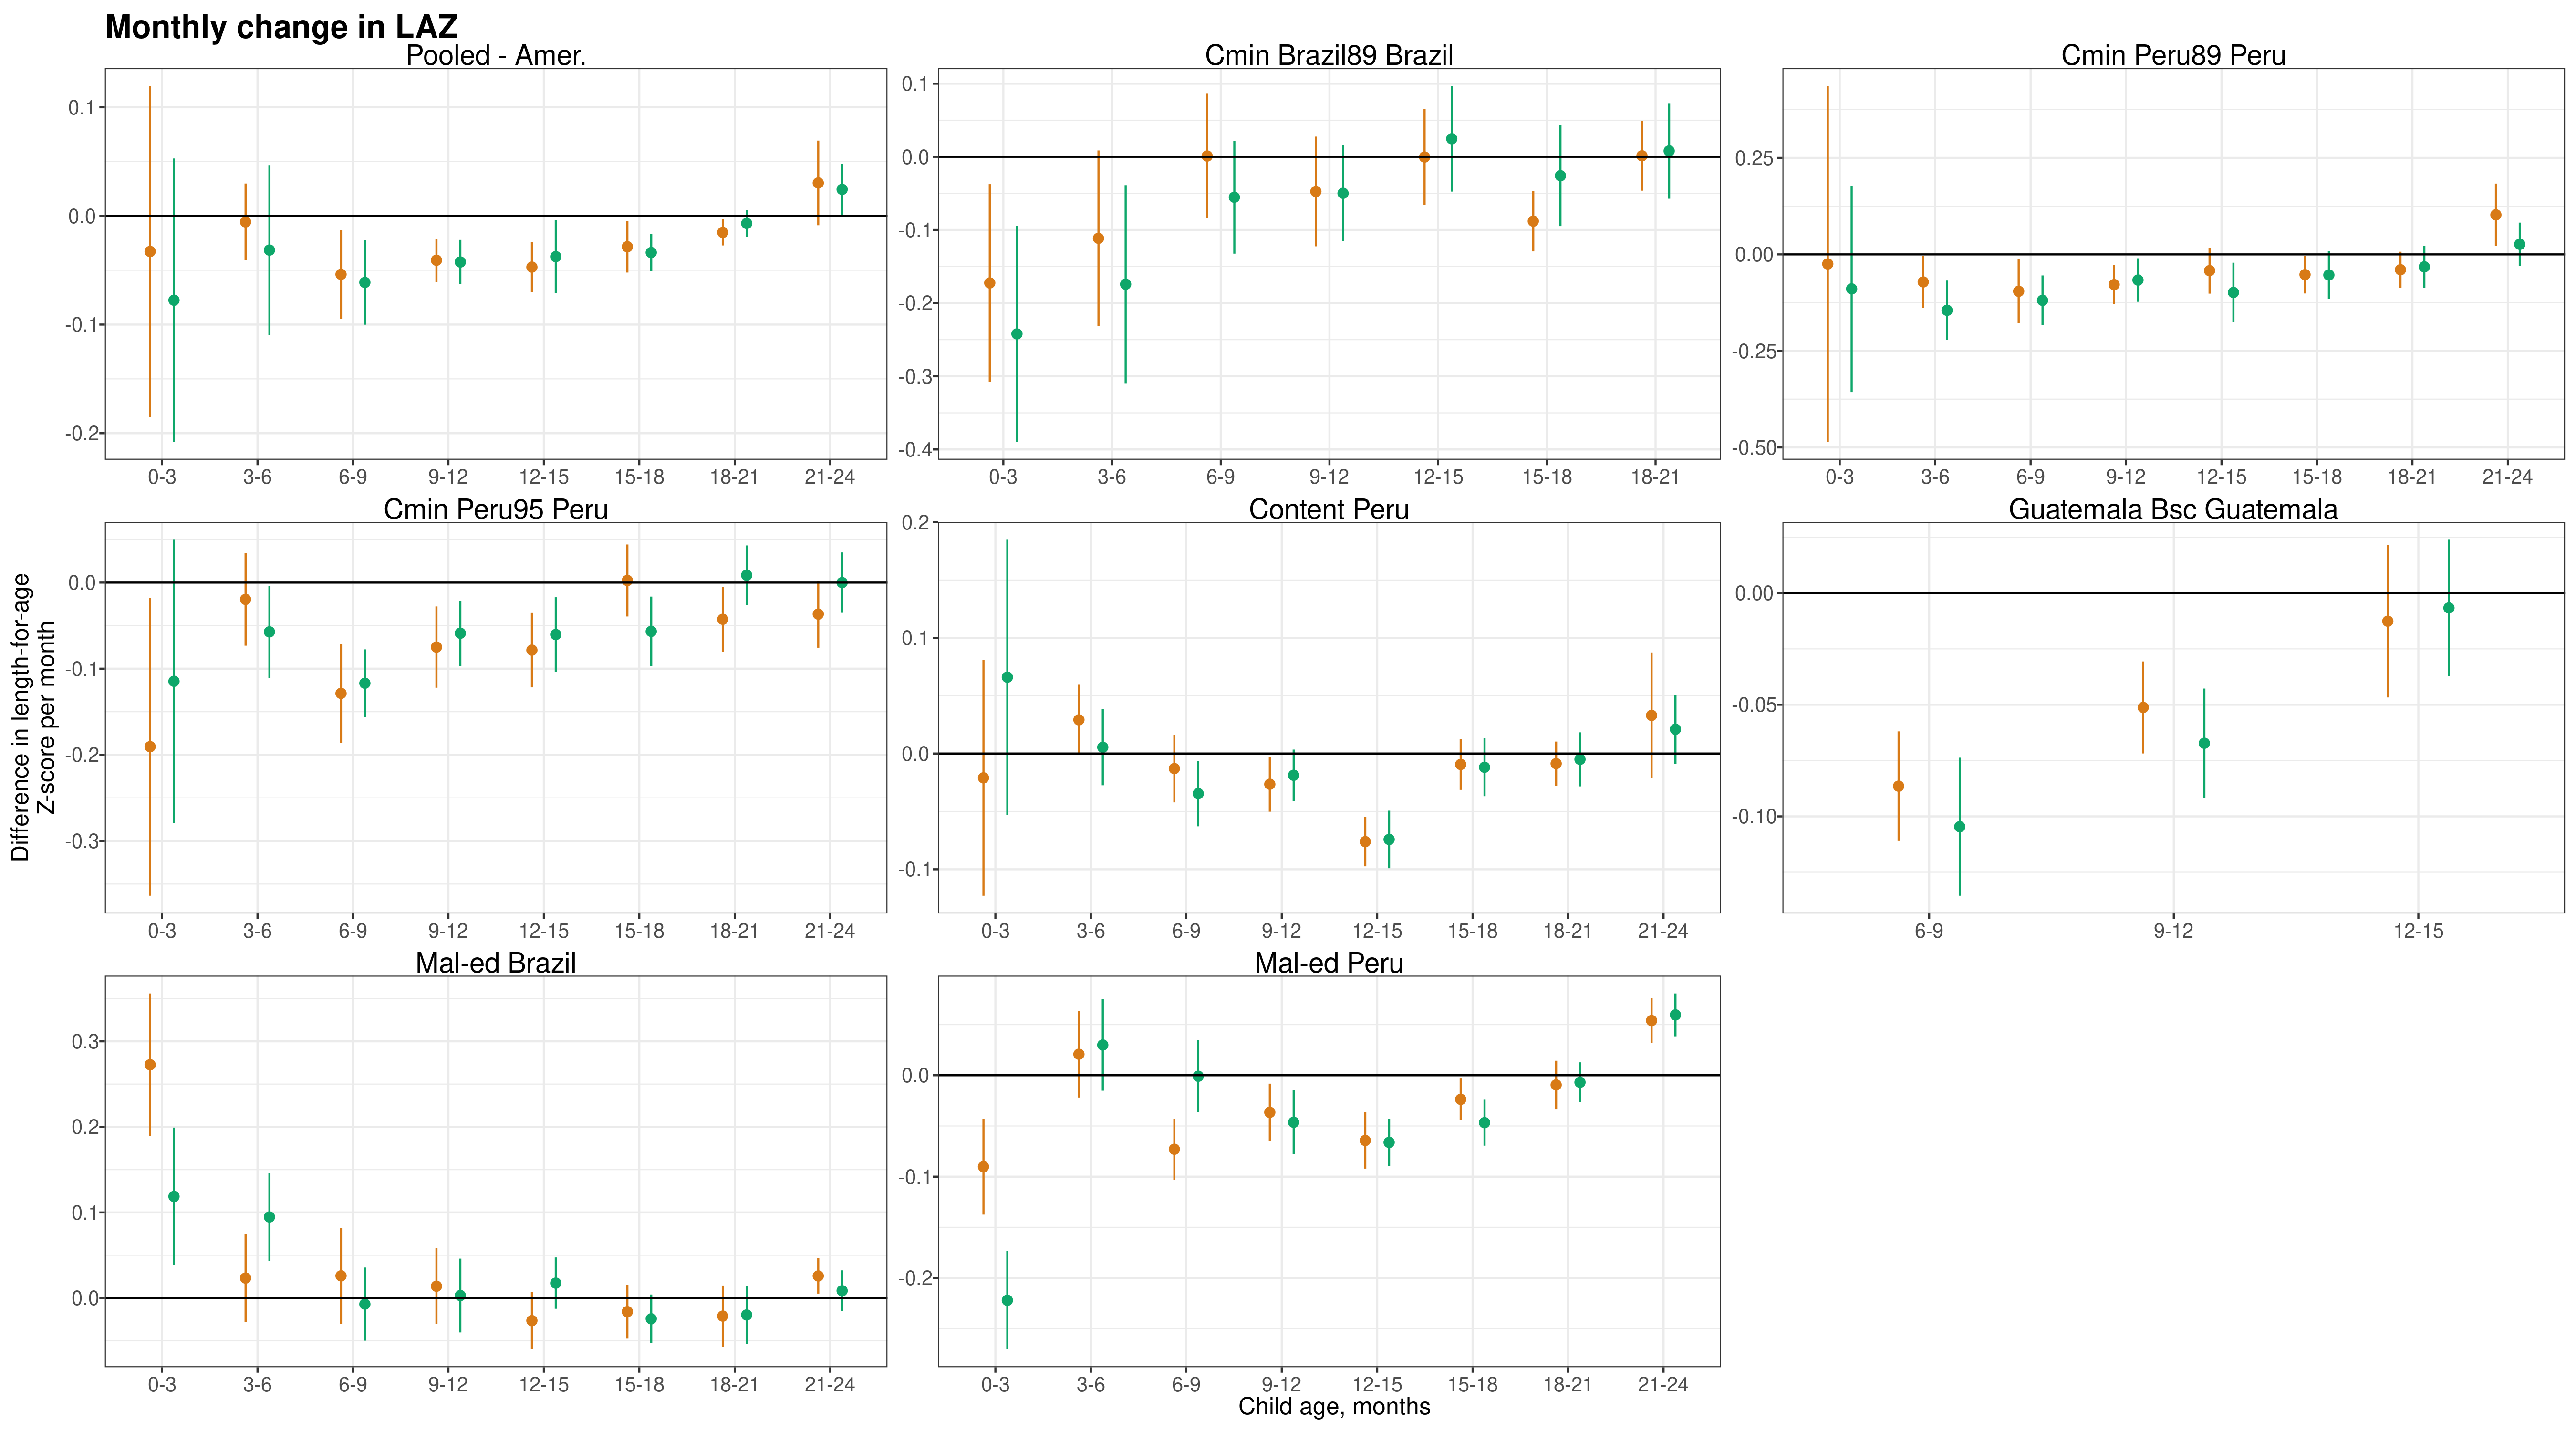
\includegraphics[width=75in]{figures//stunting/fig-laz-2-laz_vel-cohort-latamer-allage-primary}

\hypertarget{south-asia-4}{%
\subsection{South Asia}\label{south-asia-4}}

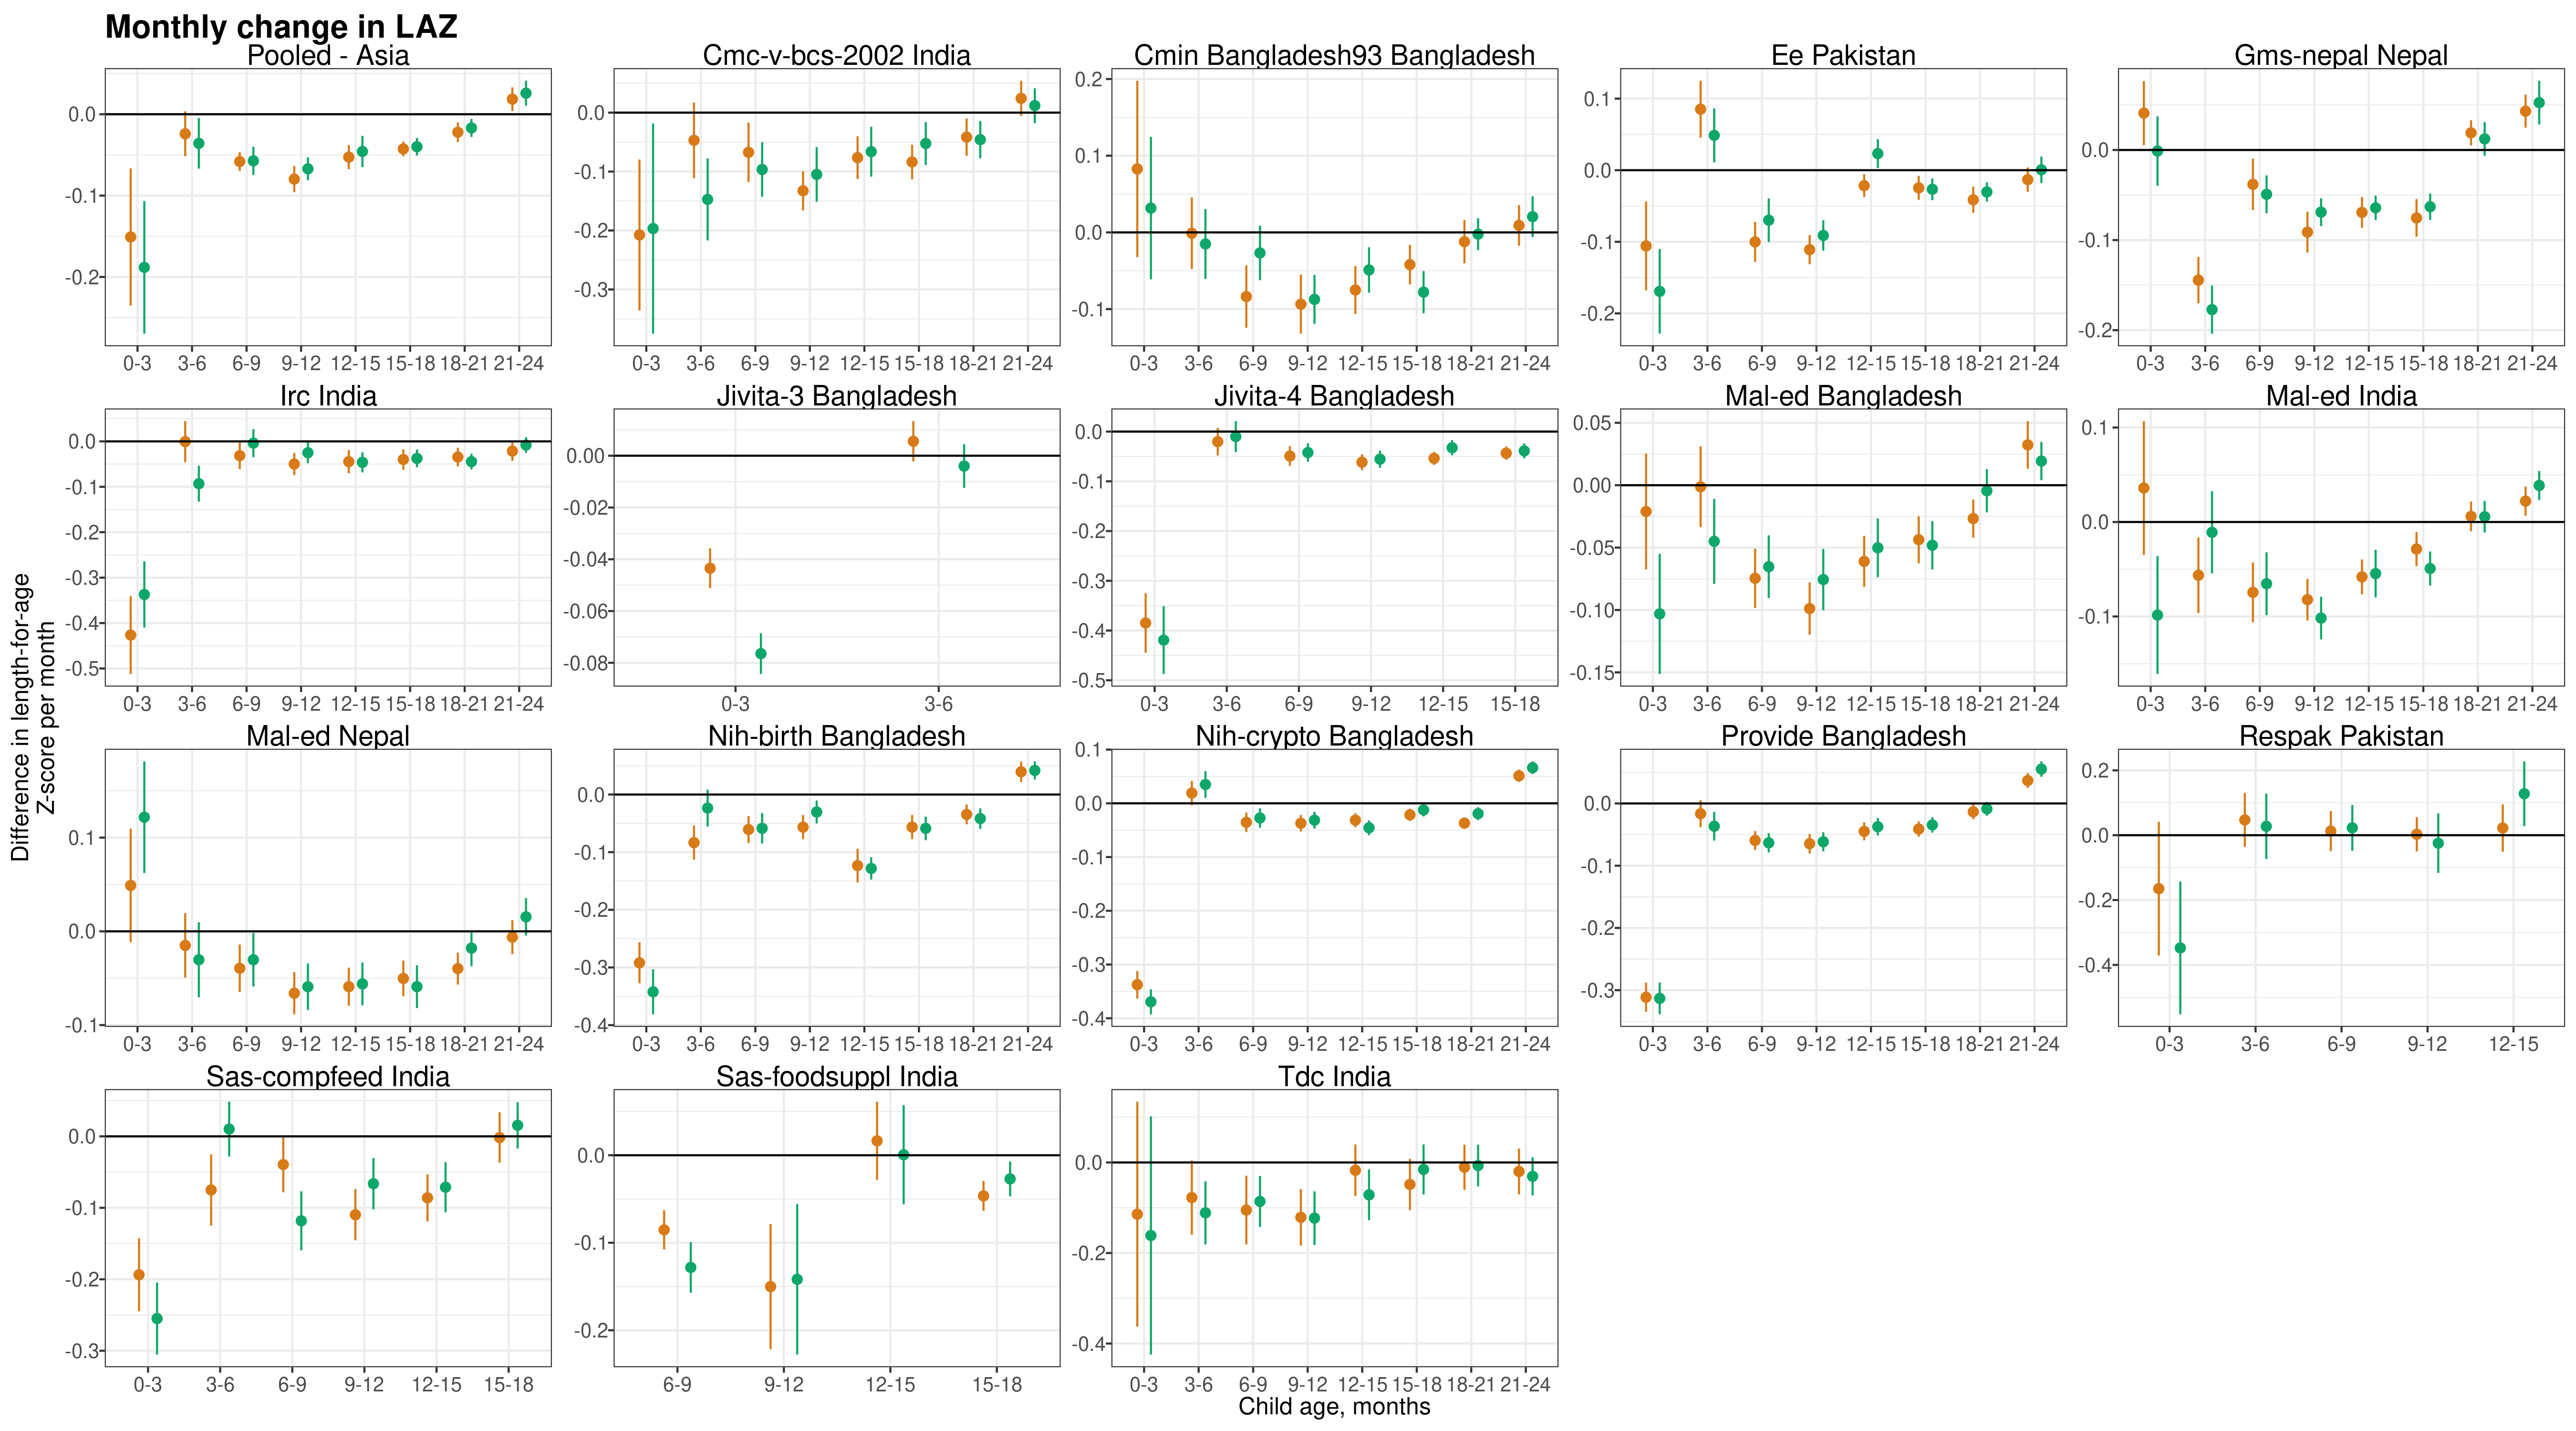
\includegraphics[width=75in]{figures//stunting/fig-laz-2-laz_vel-cohort-asia-allage-primary}

\hypertarget{exclude-PROBIT}{%
\chapter{Primary analyses excluding the PROBIT study}\label{exclude-PROBIT}}

\raggedright

Only one cohort from Europe met the inclusion criteria for this study -- the PROBIT study. To assess whether inclusion of this study altered our overall study inference, we repeated analyses excluding the PROBIT cohort, as shown below in the ``Overall'' panels. Results were very similar with and without the PROBIT cohort. Stunting prevalence and incidence were slightly higher at birth when excluding PROBIT, but overall age-specific patterns remained the same. For this reason, we chose to retain PROBIT in the primary analyses presented in this manuscript.

\hypertarget{mean-length-for-age-z-score-by-age-1}{%
\section{Mean length-for-age Z-score by age}\label{mean-length-for-age-z-score-by-age-1}}

\hypertarget{including-probit}{%
\subsection{Including PROBIT}\label{including-probit}}

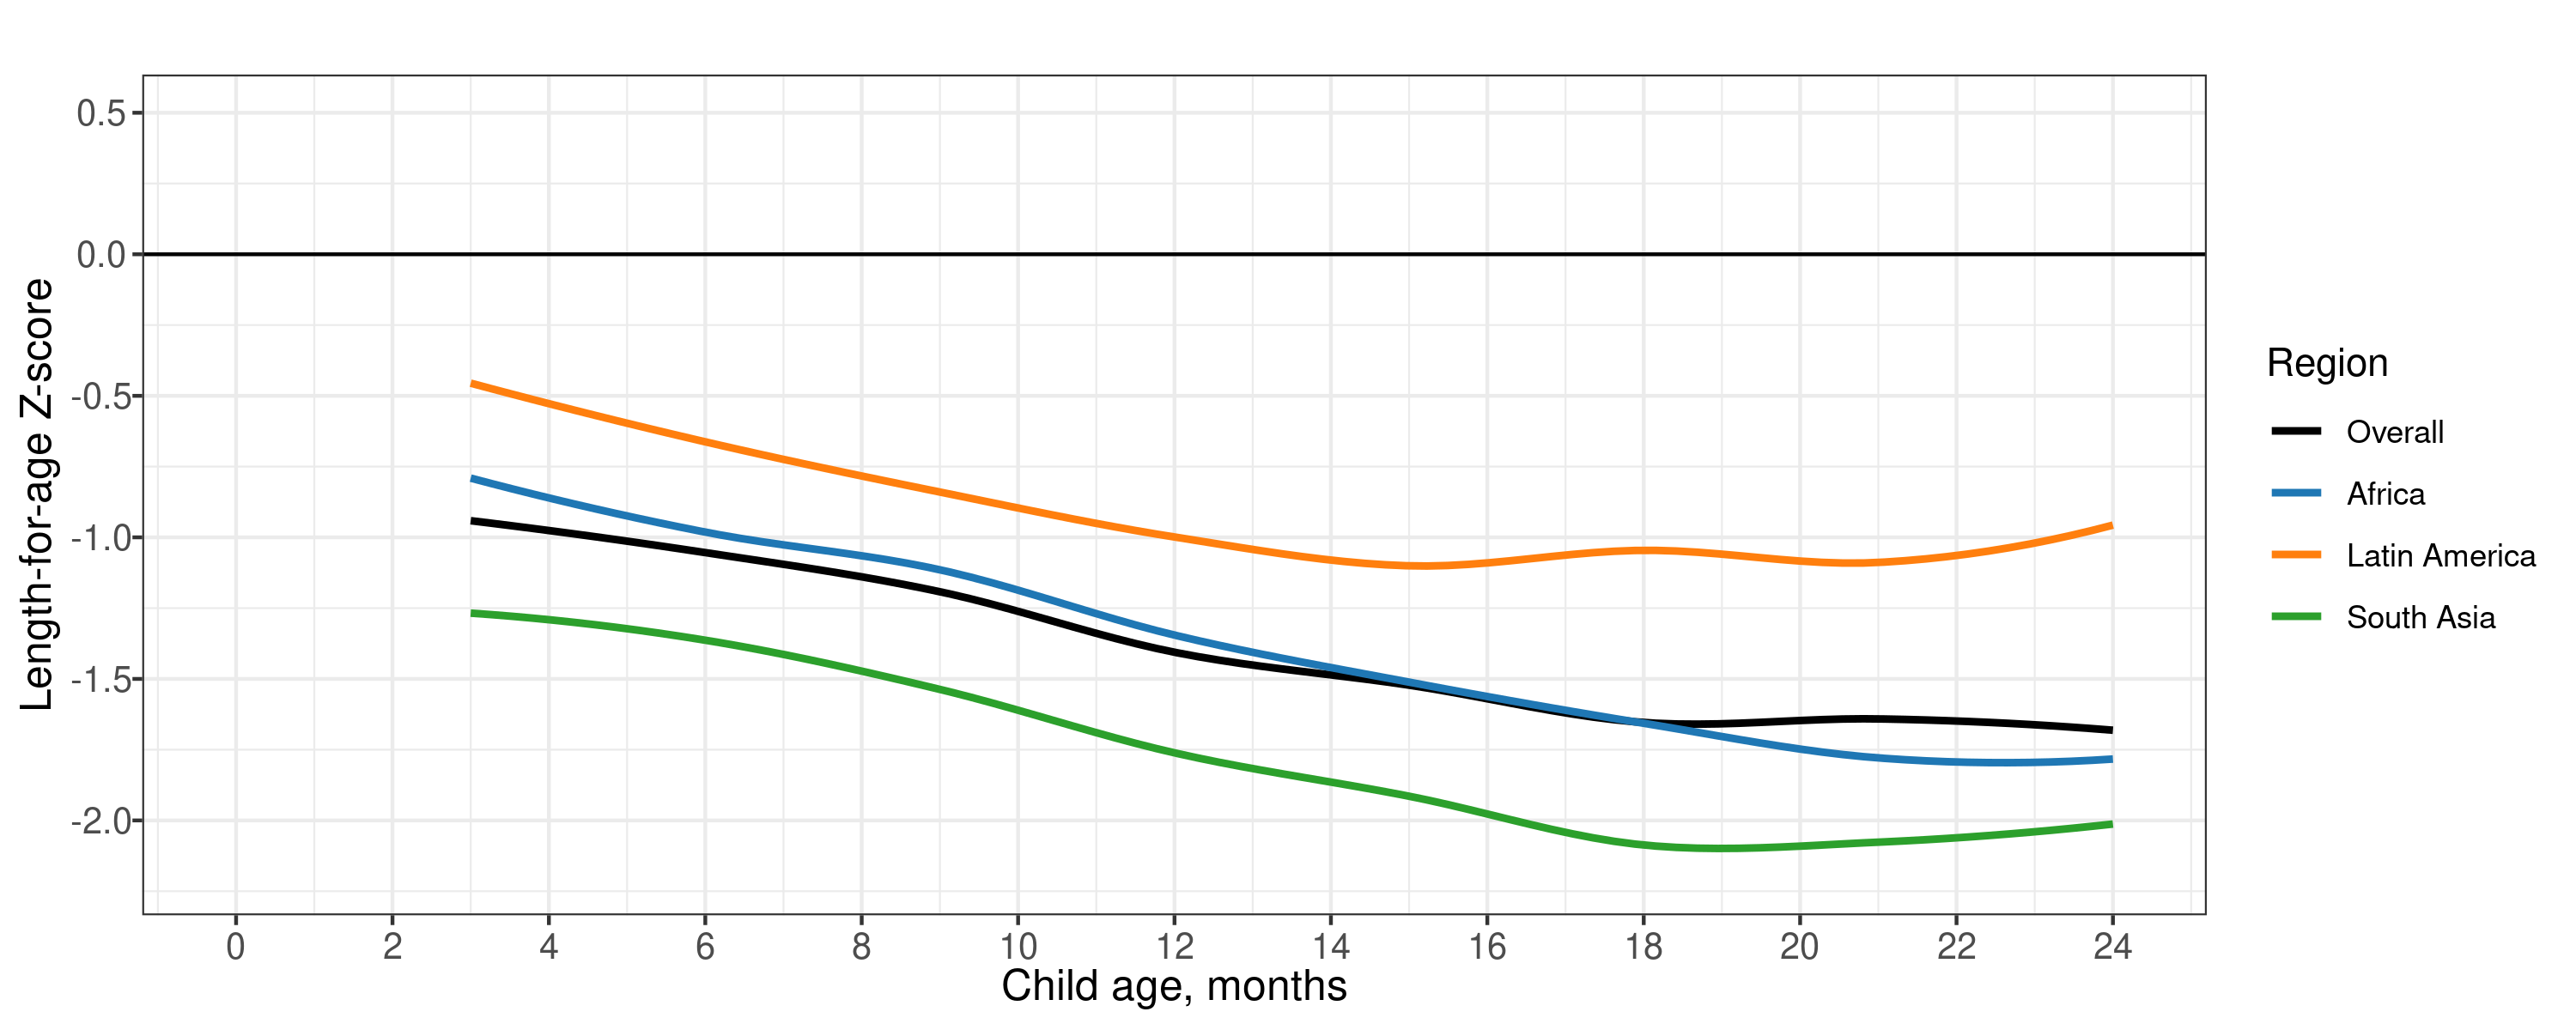
\includegraphics[width=41.67in]{figures//stunting/fig-laz-2-mean-overall_region--allage-primary}

\hypertarget{excluding-probit}{%
\subsection{Excluding PROBIT}\label{excluding-probit}}

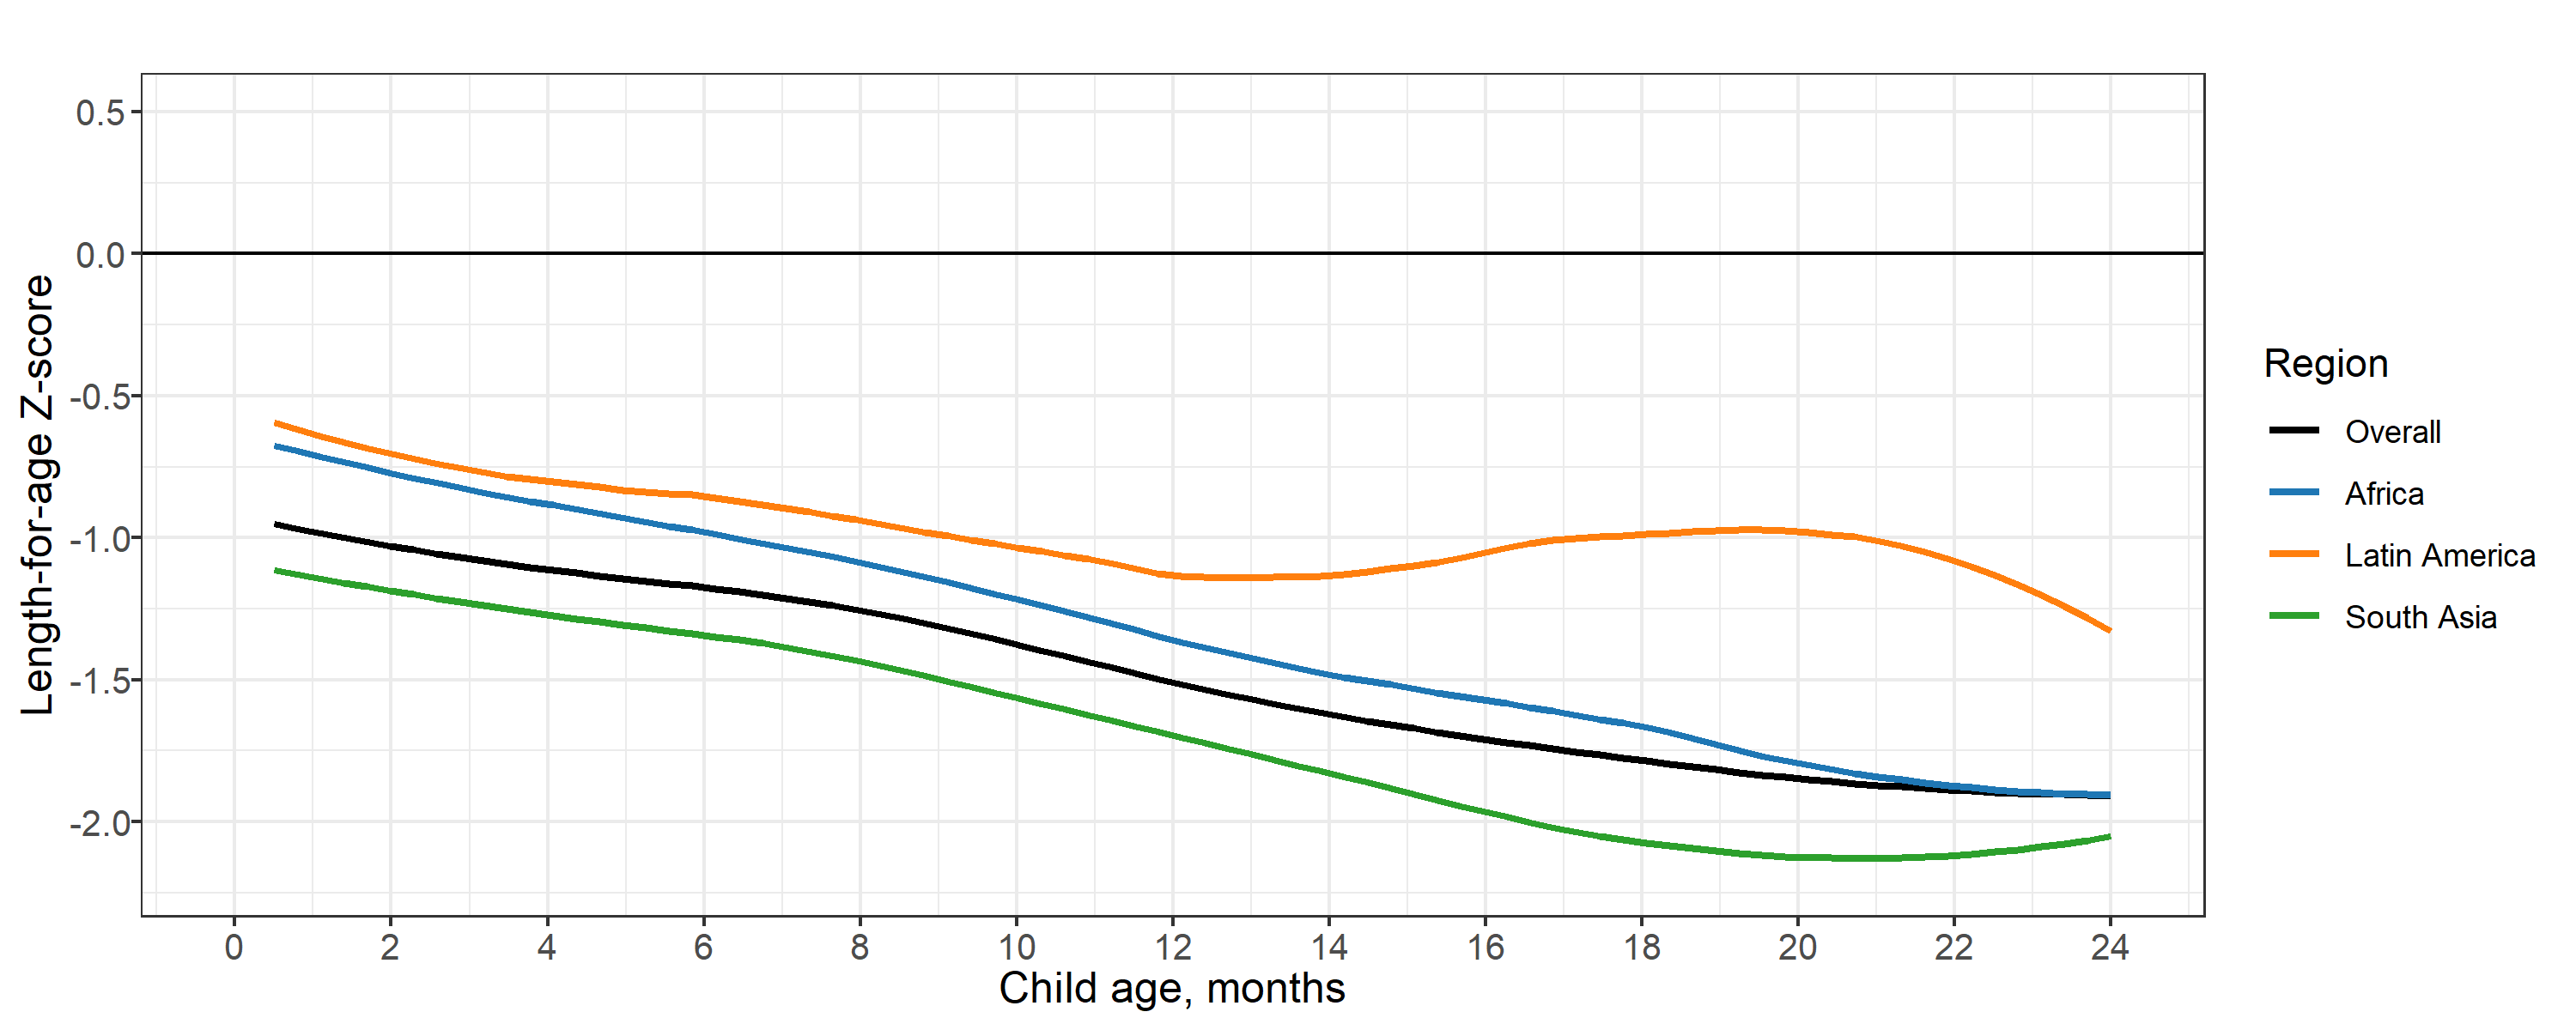
\includegraphics[width=41.67in]{figures//stunting/fig-laz-2-mean-overall_region--allage-primary_no_probit}

\hypertarget{age-specific-prevalence-1}{%
\section{Age-specific prevalence}\label{age-specific-prevalence-1}}

\hypertarget{including-probit-1}{%
\subsection{Including PROBIT}\label{including-probit-1}}

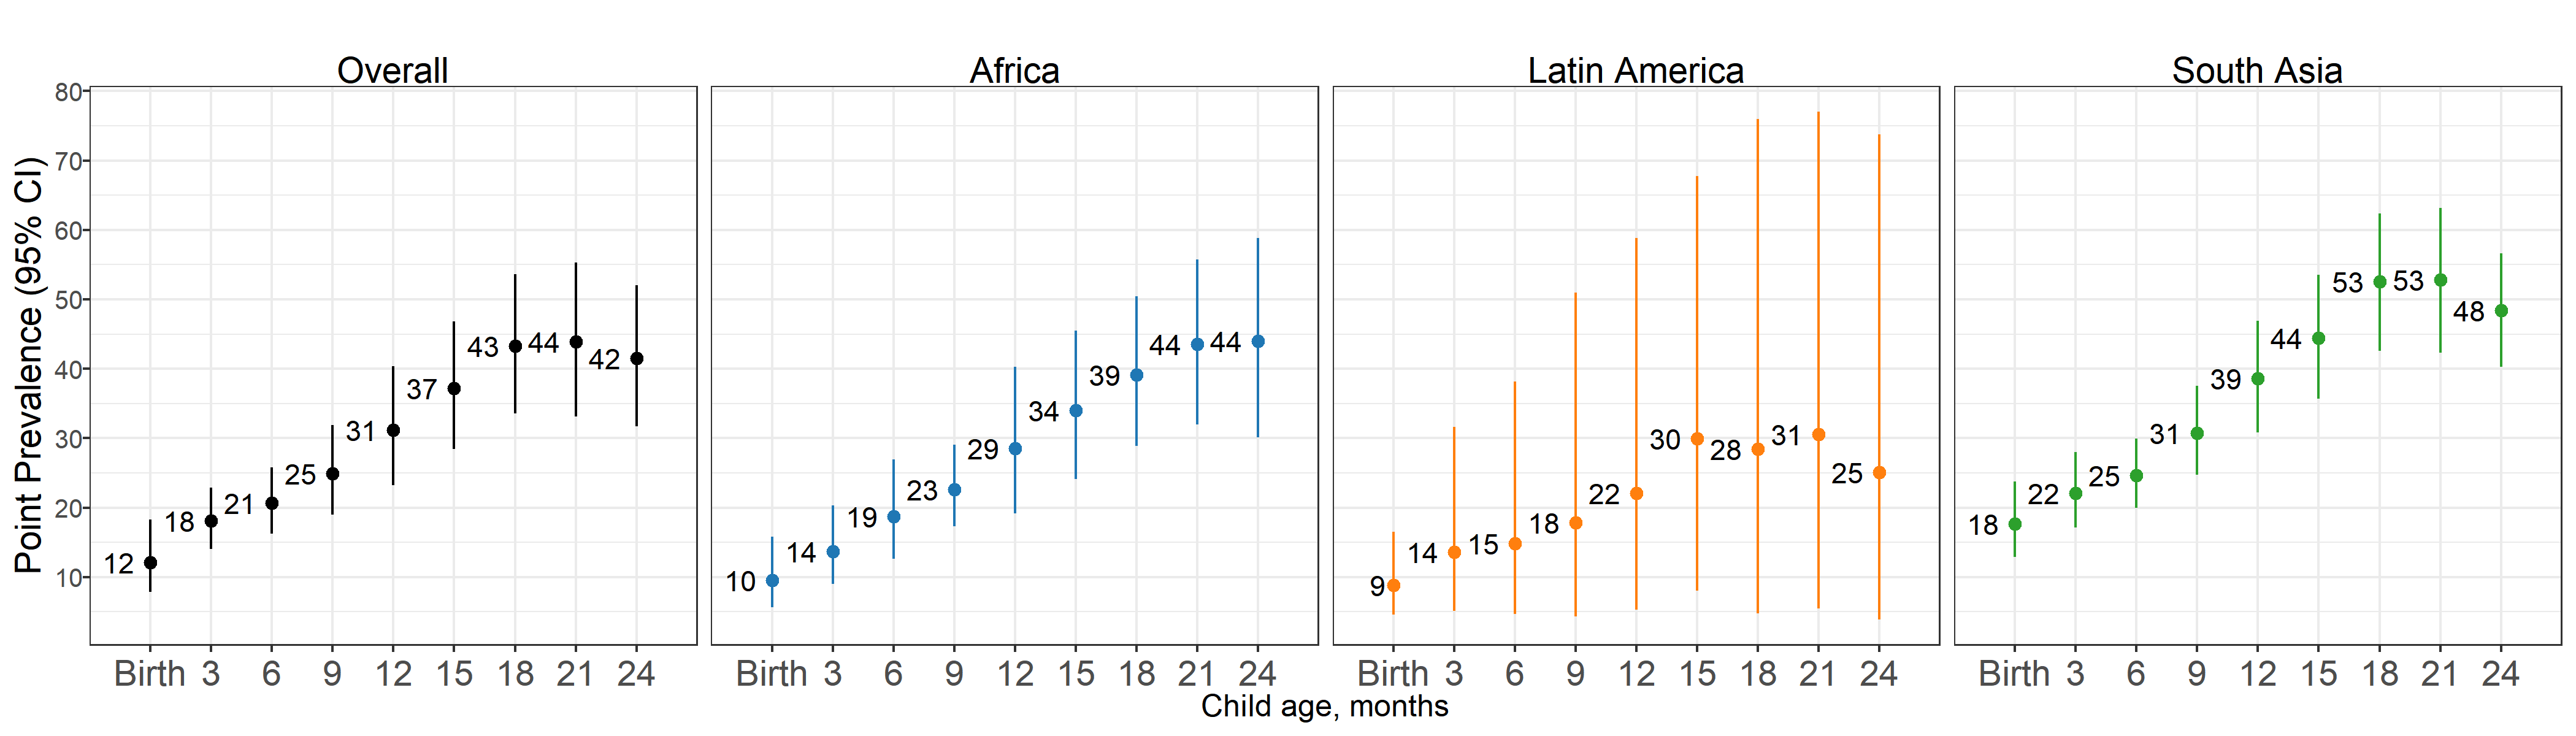
\includegraphics[width=58.33in]{figures//stunting/fig-stunt-2-prev-overall_region--allage-primary}

\hypertarget{excluding-probit-1}{%
\subsection{Excluding PROBIT}\label{excluding-probit-1}}

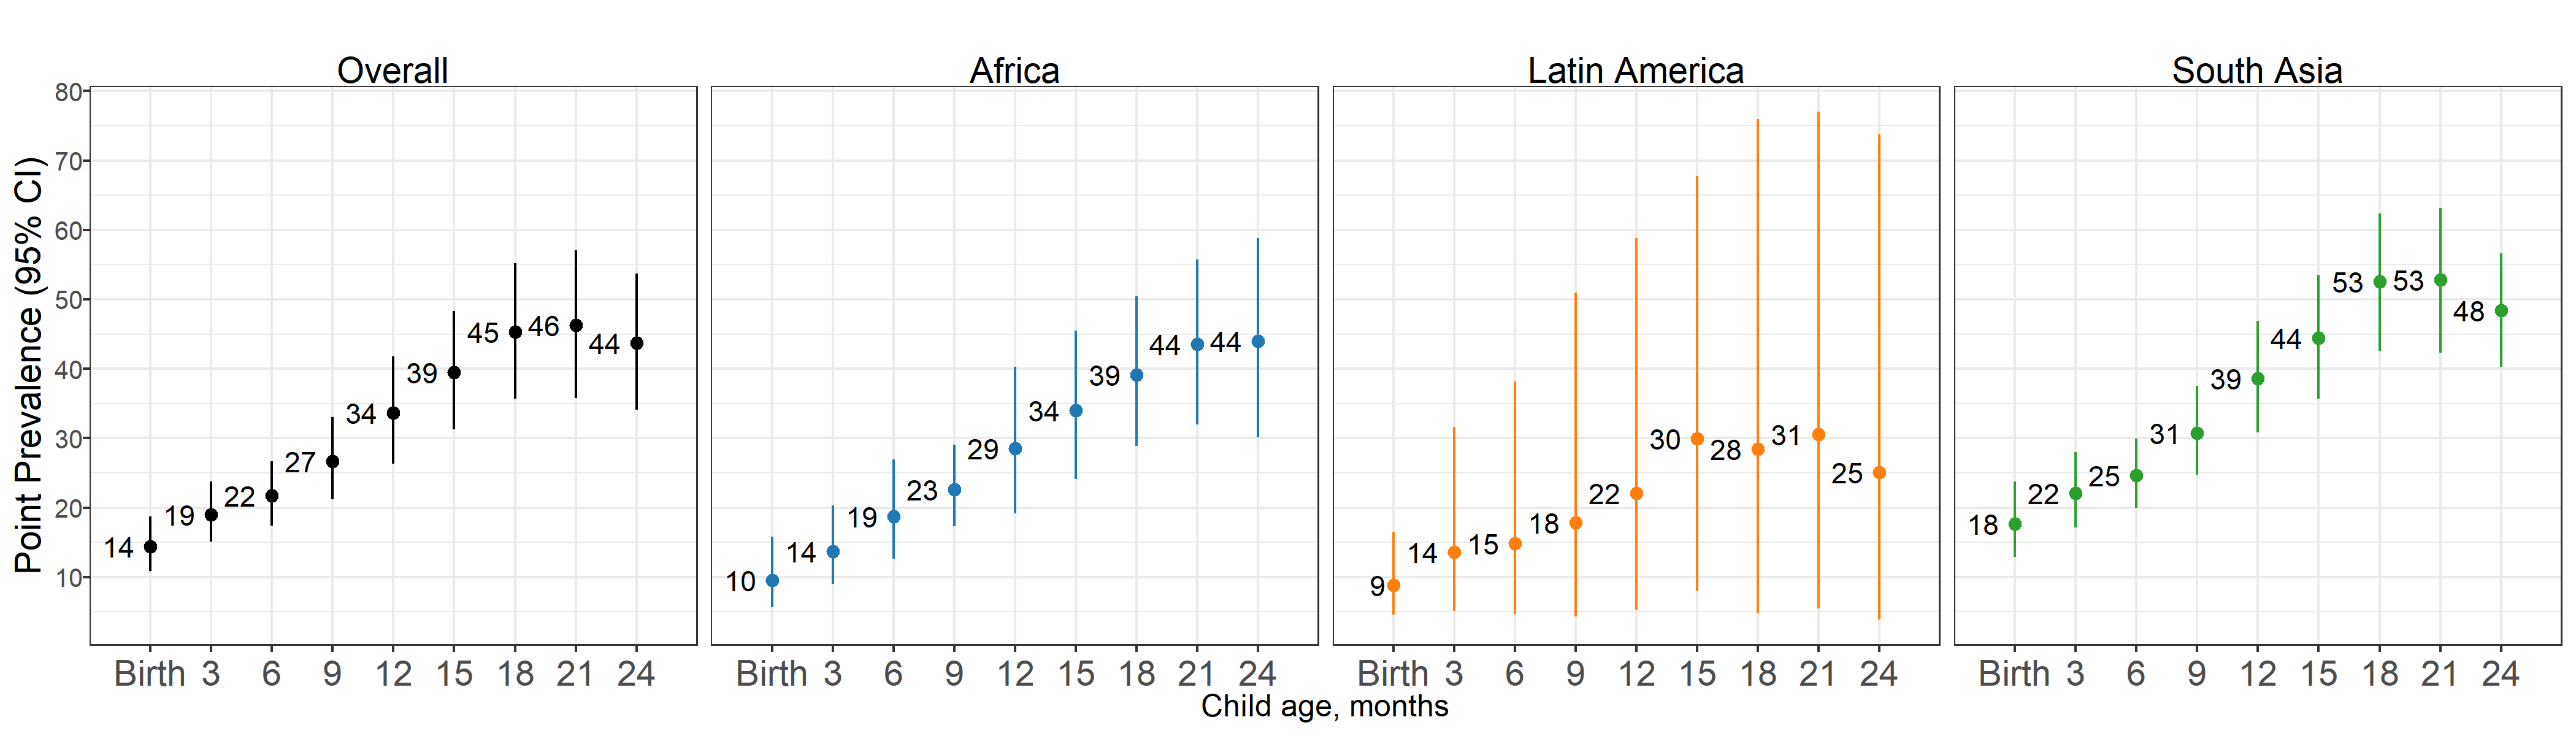
\includegraphics[width=58.33in]{figures//stunting/fig-stunt-2-prev-overall_region--allage-primary_no_probit}

\hypertarget{age-specific-incidence-1}{%
\section{Age-specific incidence}\label{age-specific-incidence-1}}

\hypertarget{including-probit-2}{%
\subsection{Including PROBIT}\label{including-probit-2}}

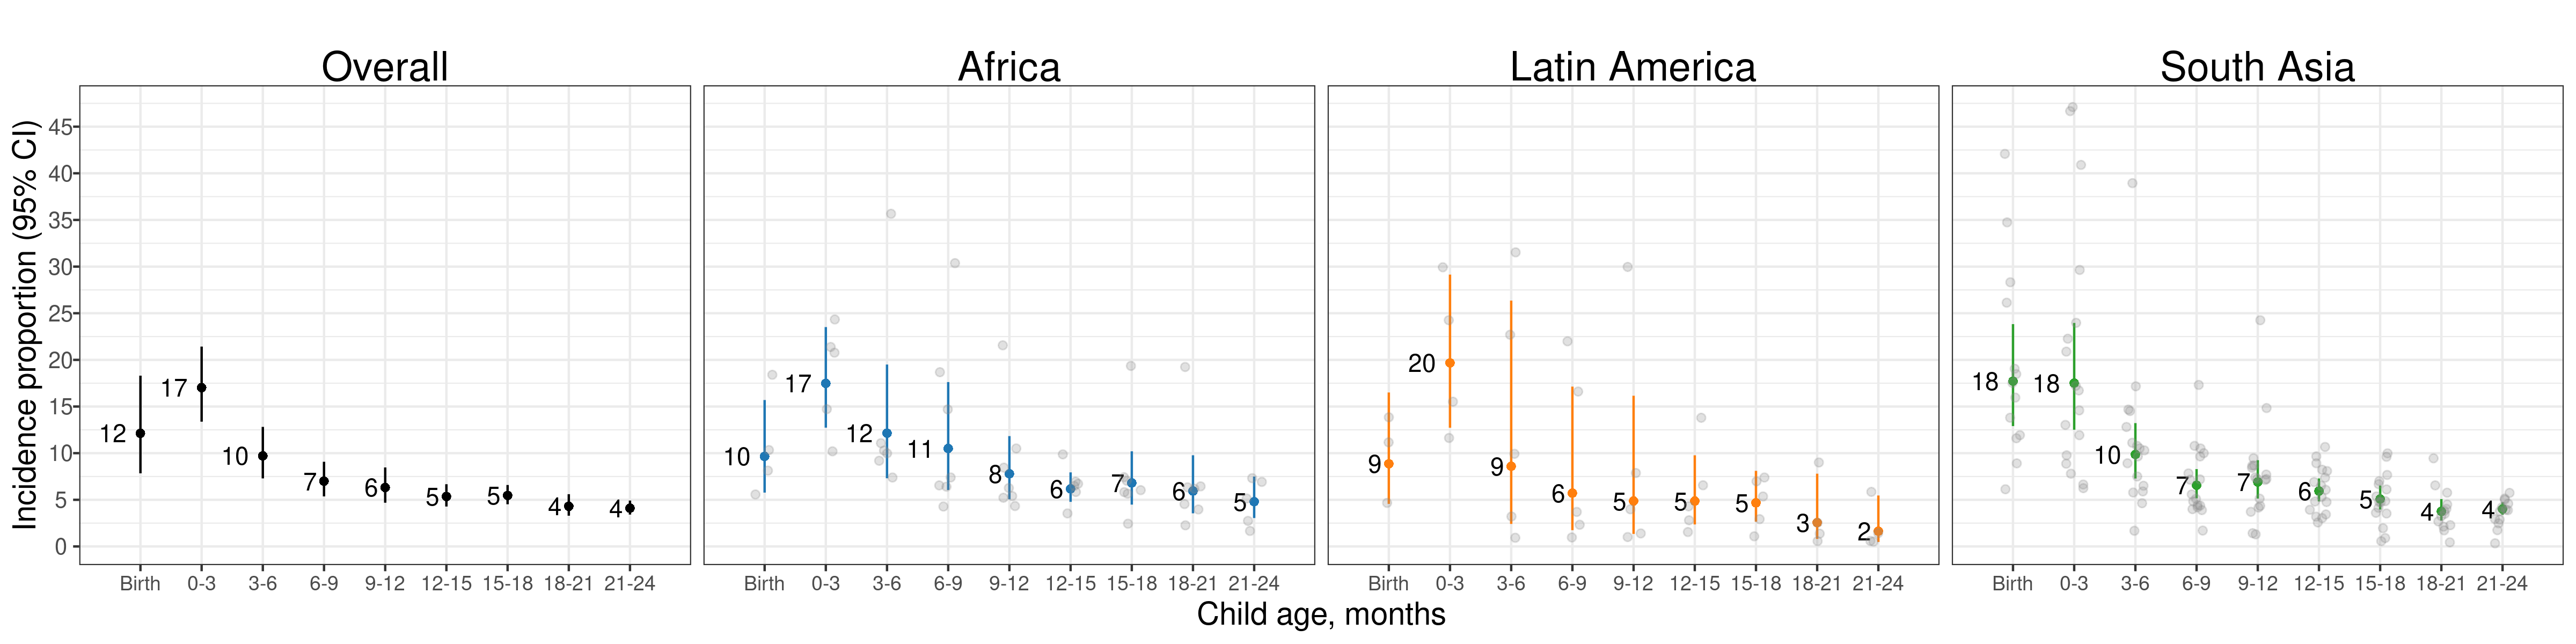
\includegraphics[width=66.67in]{figures//stunting/fig-stunt-2-inc-overall_region--allage-primary}

\hypertarget{excluding-probit-2}{%
\subsection{Excluding PROBIT}\label{excluding-probit-2}}

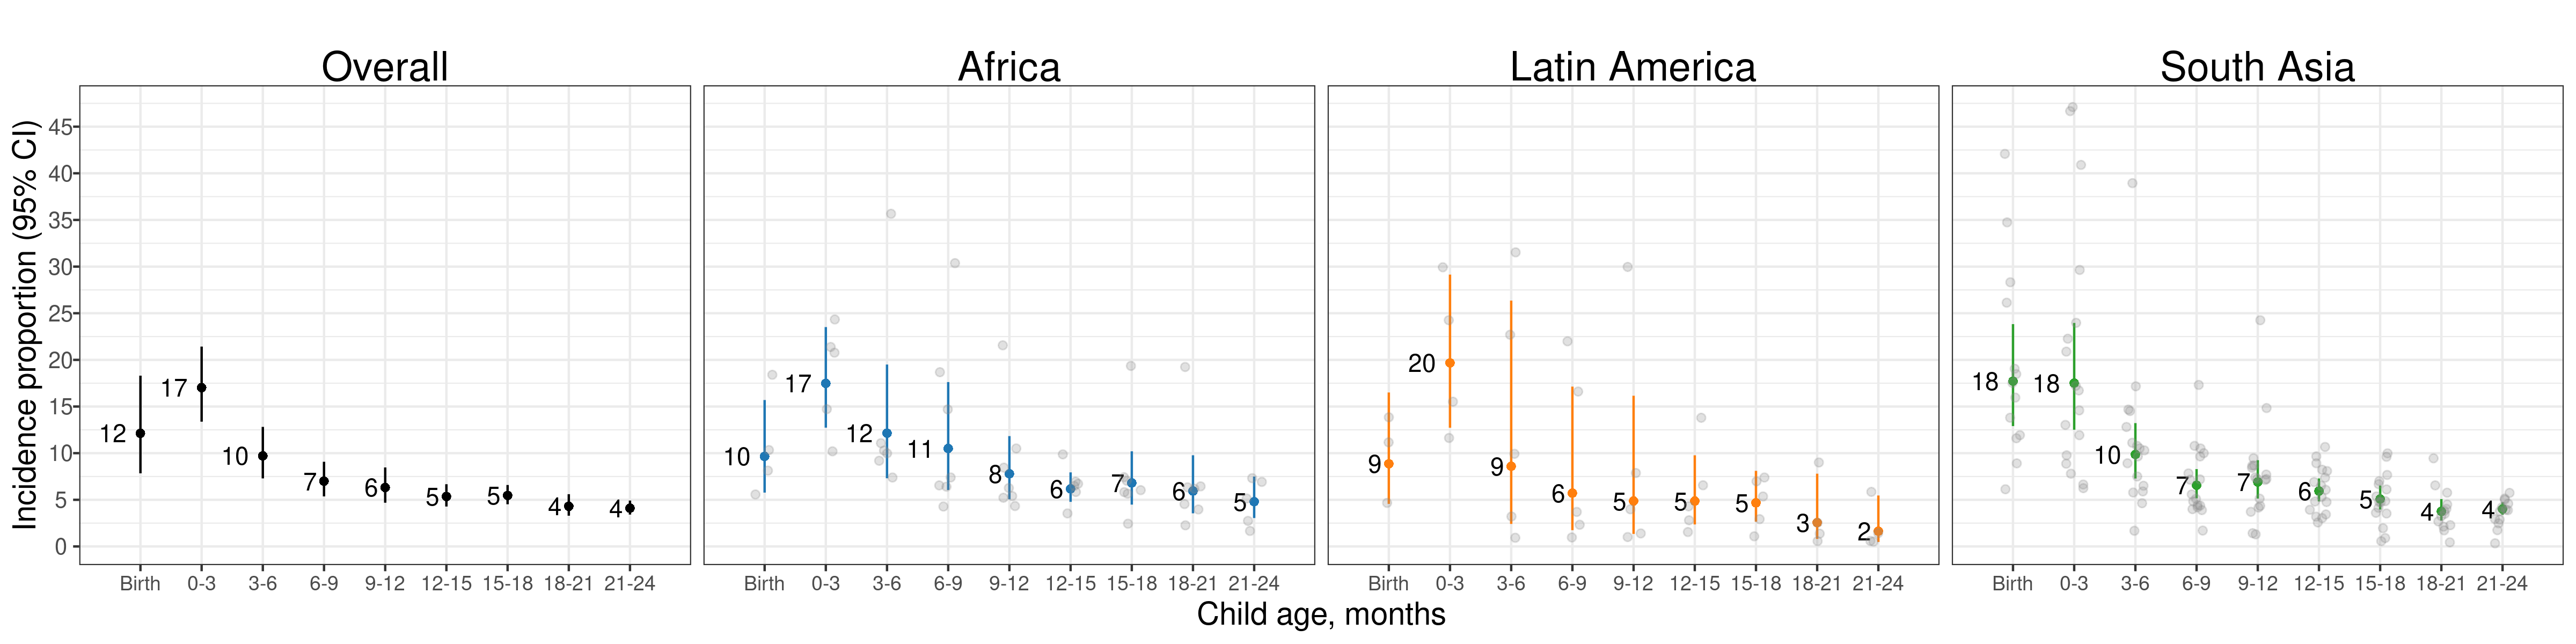
\includegraphics[width=66.67in]{figures//stunting/fig-stunt-2-inc-overall_region--allage-primary}

\hypertarget{monthly}{%
\chapter{Analysis with monthly cohorts}\label{monthly}}

\raggedright

To explore the influence of differing numbers of cohorts contributing data at different ages, we conducted a sensitivity analysis in which we subset data to cohorts that measured anthropometry monthly from birth to 24 months.

In this sensitivity analysis, the mean length-for-age Z-score was higher in Latin America and exhibited less of a downwards trajectory with age. Age-specific stunting prevalence and incidence was slightly lower in Latin America and Asia and slightly higher in Africa. Standard errors were smaller for Latin America because the analyses with monthly cohorts excluded the COHORTS Guatemala study, which had a very high stunting prevalence compared to other Latin American cohorts.

\hypertarget{mean-length-for-age-z-score-by-age-2}{%
\section{Mean length-for-age Z-score by age}\label{mean-length-for-age-z-score-by-age-2}}

\hypertarget{all-eligible-cohorts}{%
\subsection{All eligible cohorts}\label{all-eligible-cohorts}}

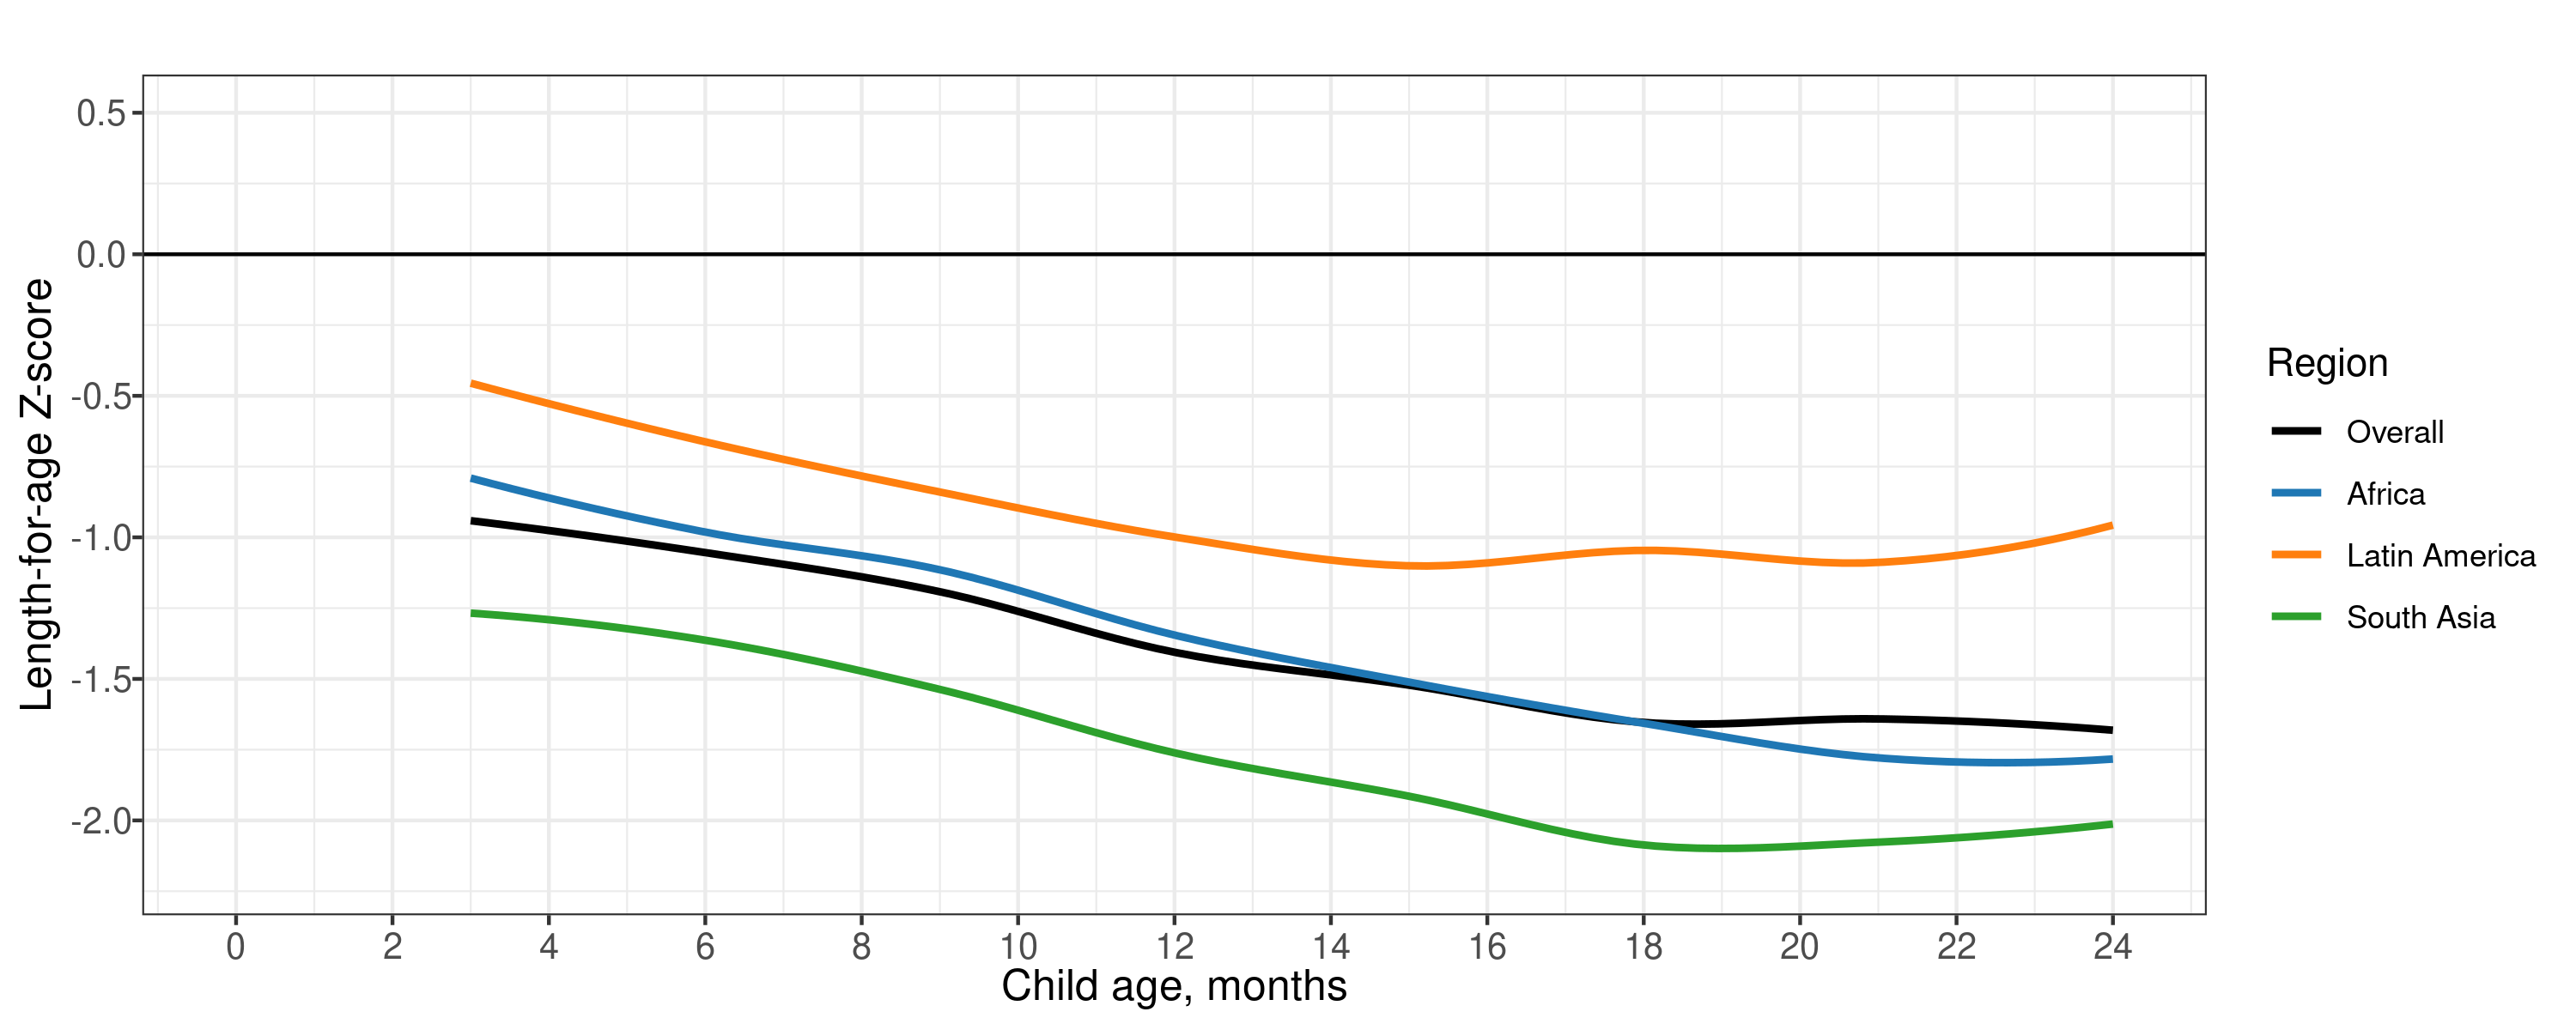
\includegraphics[width=41.67in]{figures//stunting/fig-laz-2-mean-overall_region--allage-primary}

\hypertarget{cohorts-that-measured-monthly-from-birth-to-24-months}{%
\subsection{Cohorts that measured monthly from birth to 24 months}\label{cohorts-that-measured-monthly-from-birth-to-24-months}}

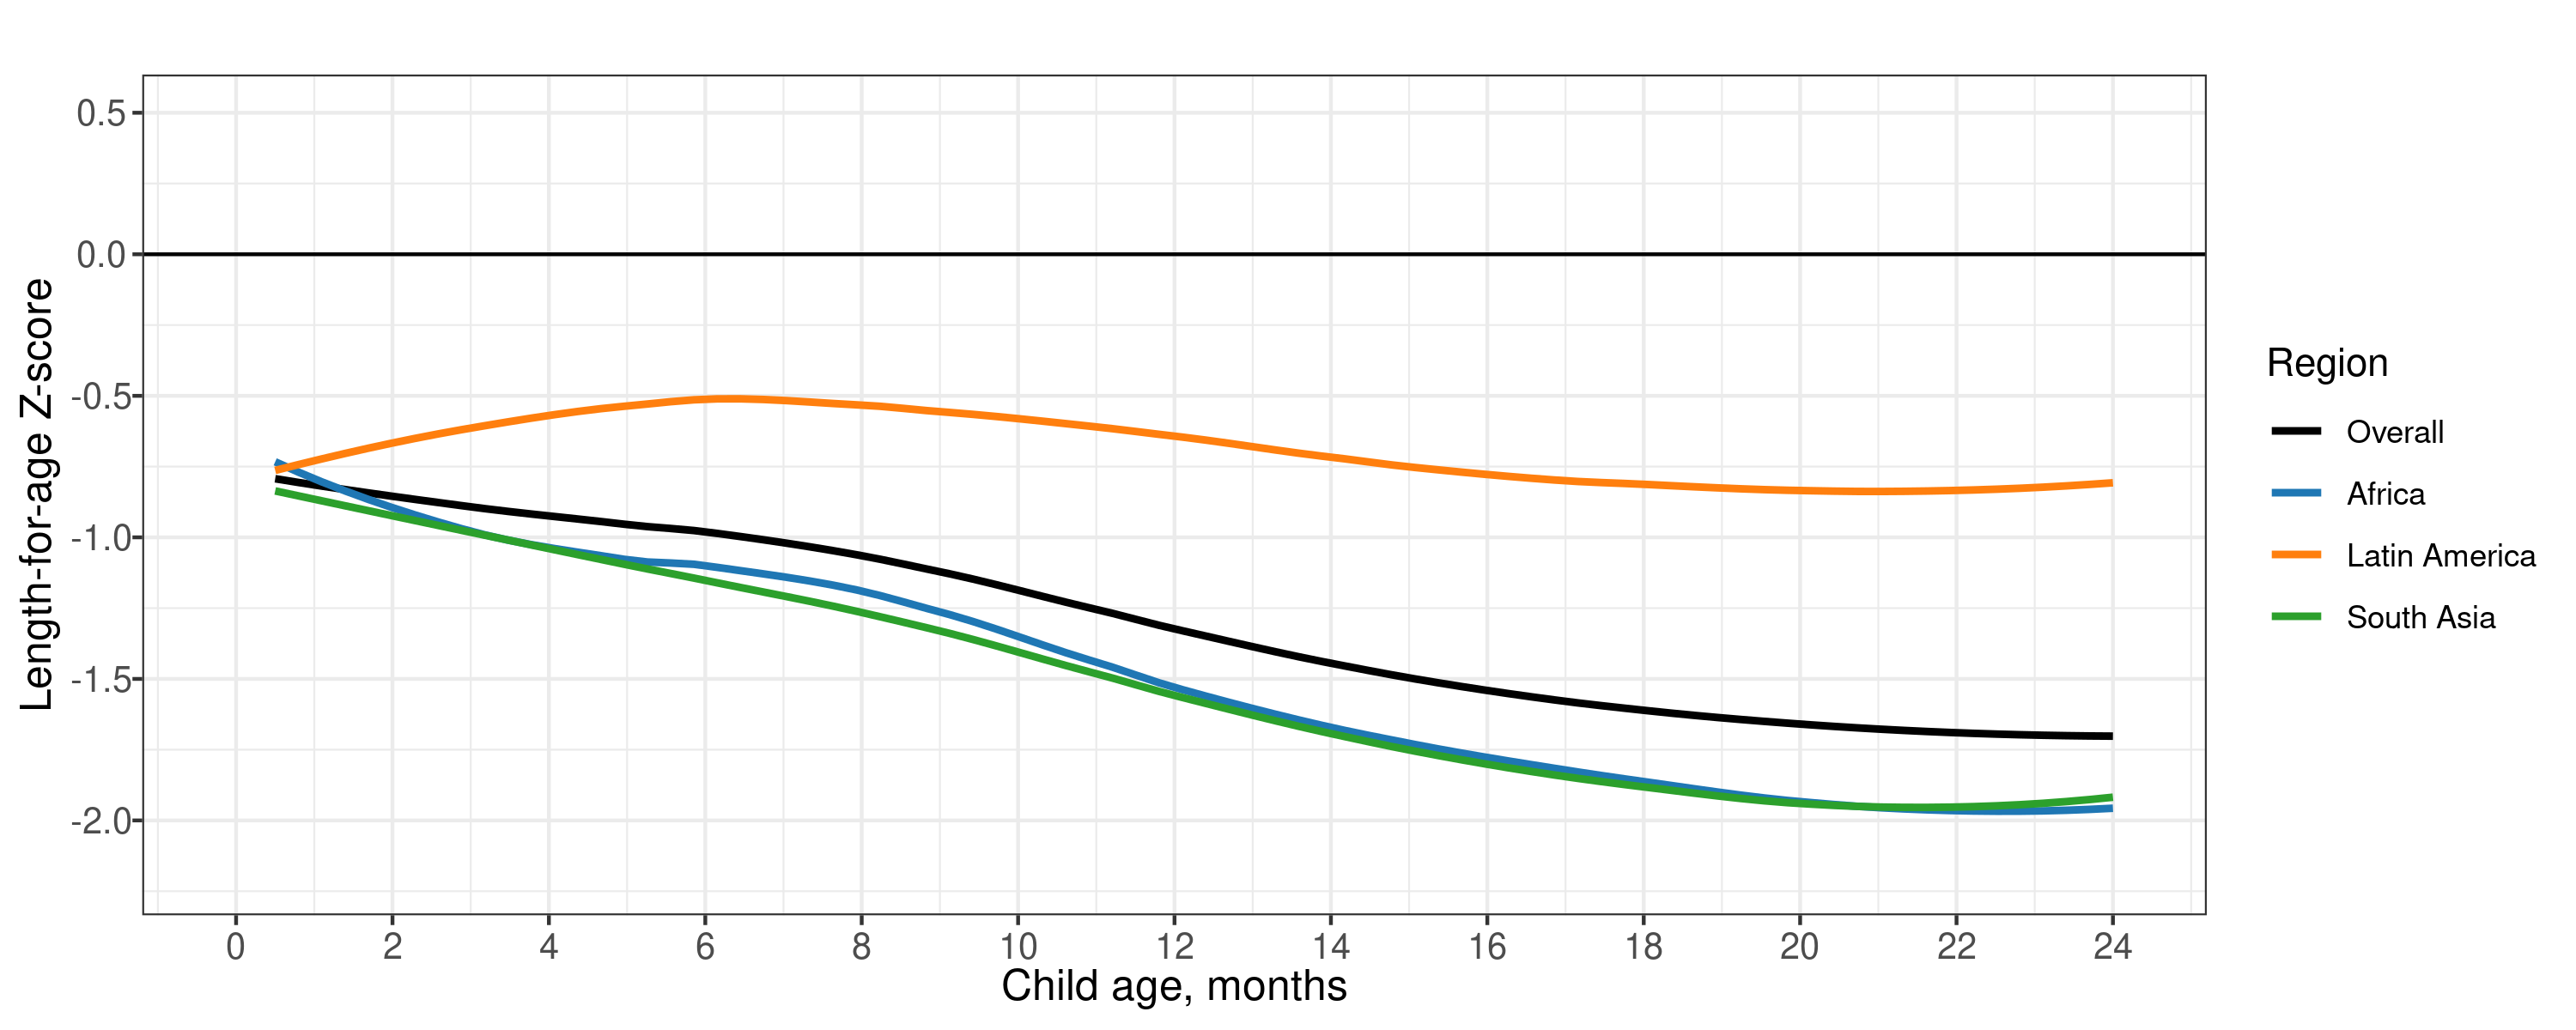
\includegraphics[width=41.67in]{figures//stunting/fig-laz-2-mean-overall_region--allage-month24}

\hypertarget{age-specific-stunting-prevalence}{%
\section{Age-specific stunting prevalence}\label{age-specific-stunting-prevalence}}

\hypertarget{all-eligible-cohorts-1}{%
\subsection{All eligible cohorts}\label{all-eligible-cohorts-1}}

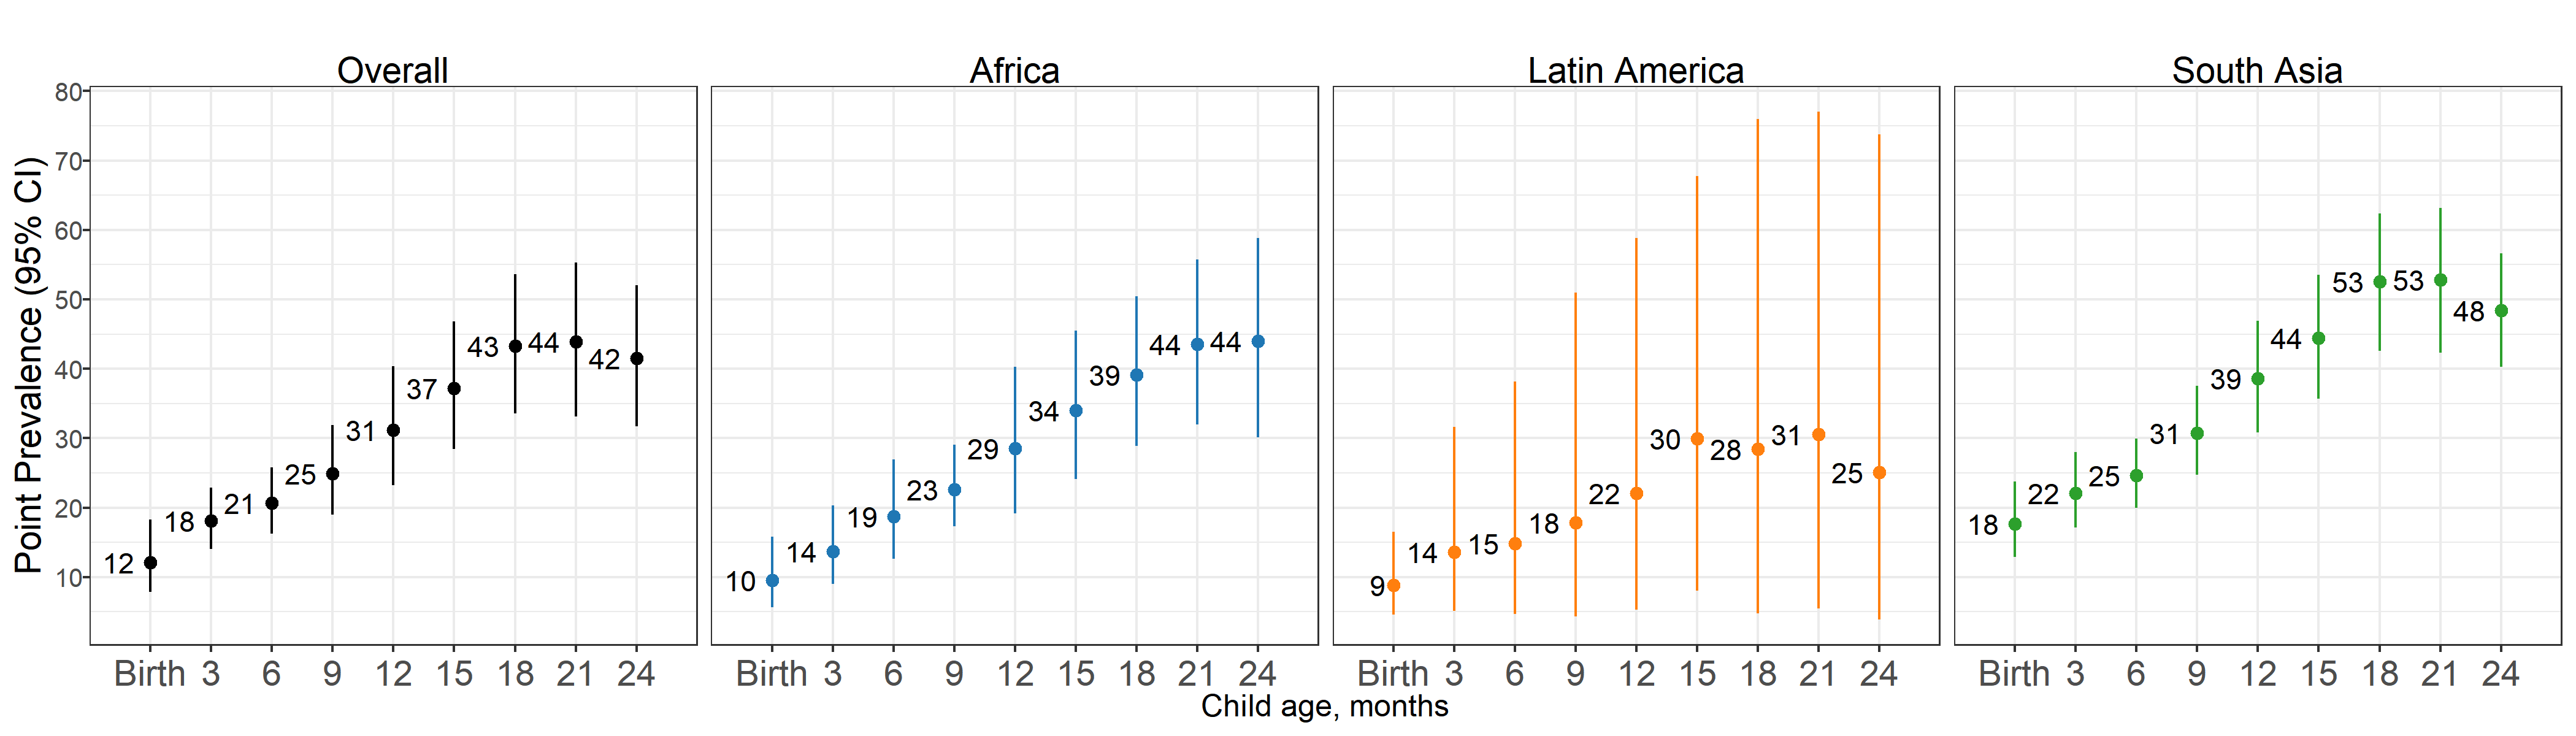
\includegraphics[width=58.33in]{figures//stunting/fig-stunt-2-prev-overall_region--allage-primary}

\hypertarget{cohorts-that-measured-monthly-from-birth-to-24-months-1}{%
\subsection{Cohorts that measured monthly from birth to 24 months}\label{cohorts-that-measured-monthly-from-birth-to-24-months-1}}

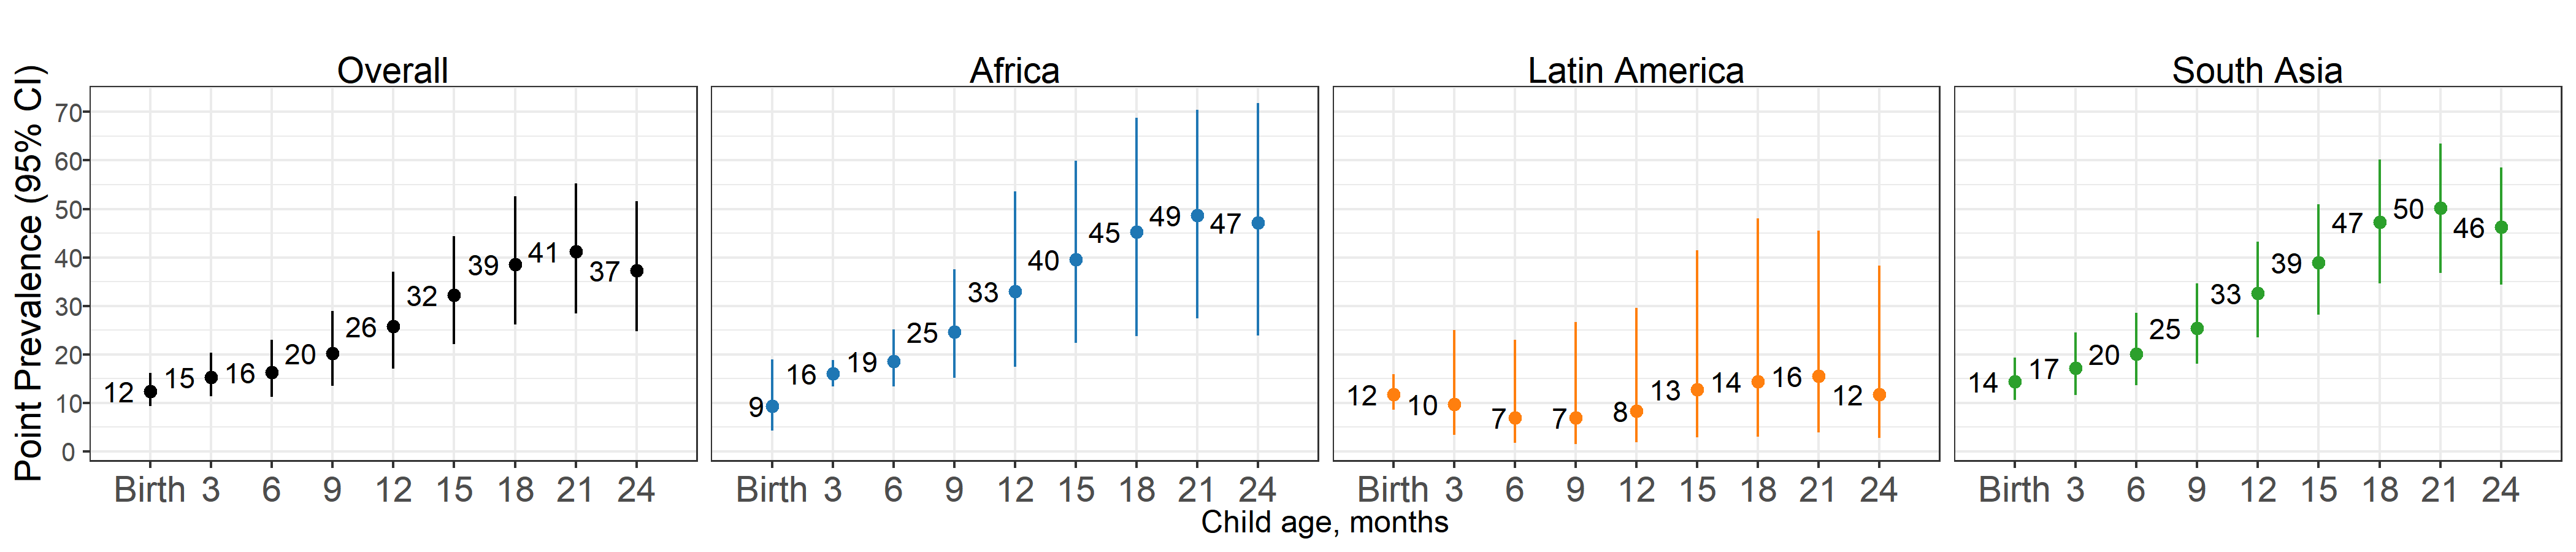
\includegraphics[width=58.33in]{figures//stunting/fig-stunt-2-prev-overall_region--allage-month24}

\hypertarget{age-specific-stunting-incidence}{%
\section{Age-specific stunting incidence}\label{age-specific-stunting-incidence}}

\hypertarget{all-eligible-cohorts-2}{%
\subsection{All eligible cohorts}\label{all-eligible-cohorts-2}}

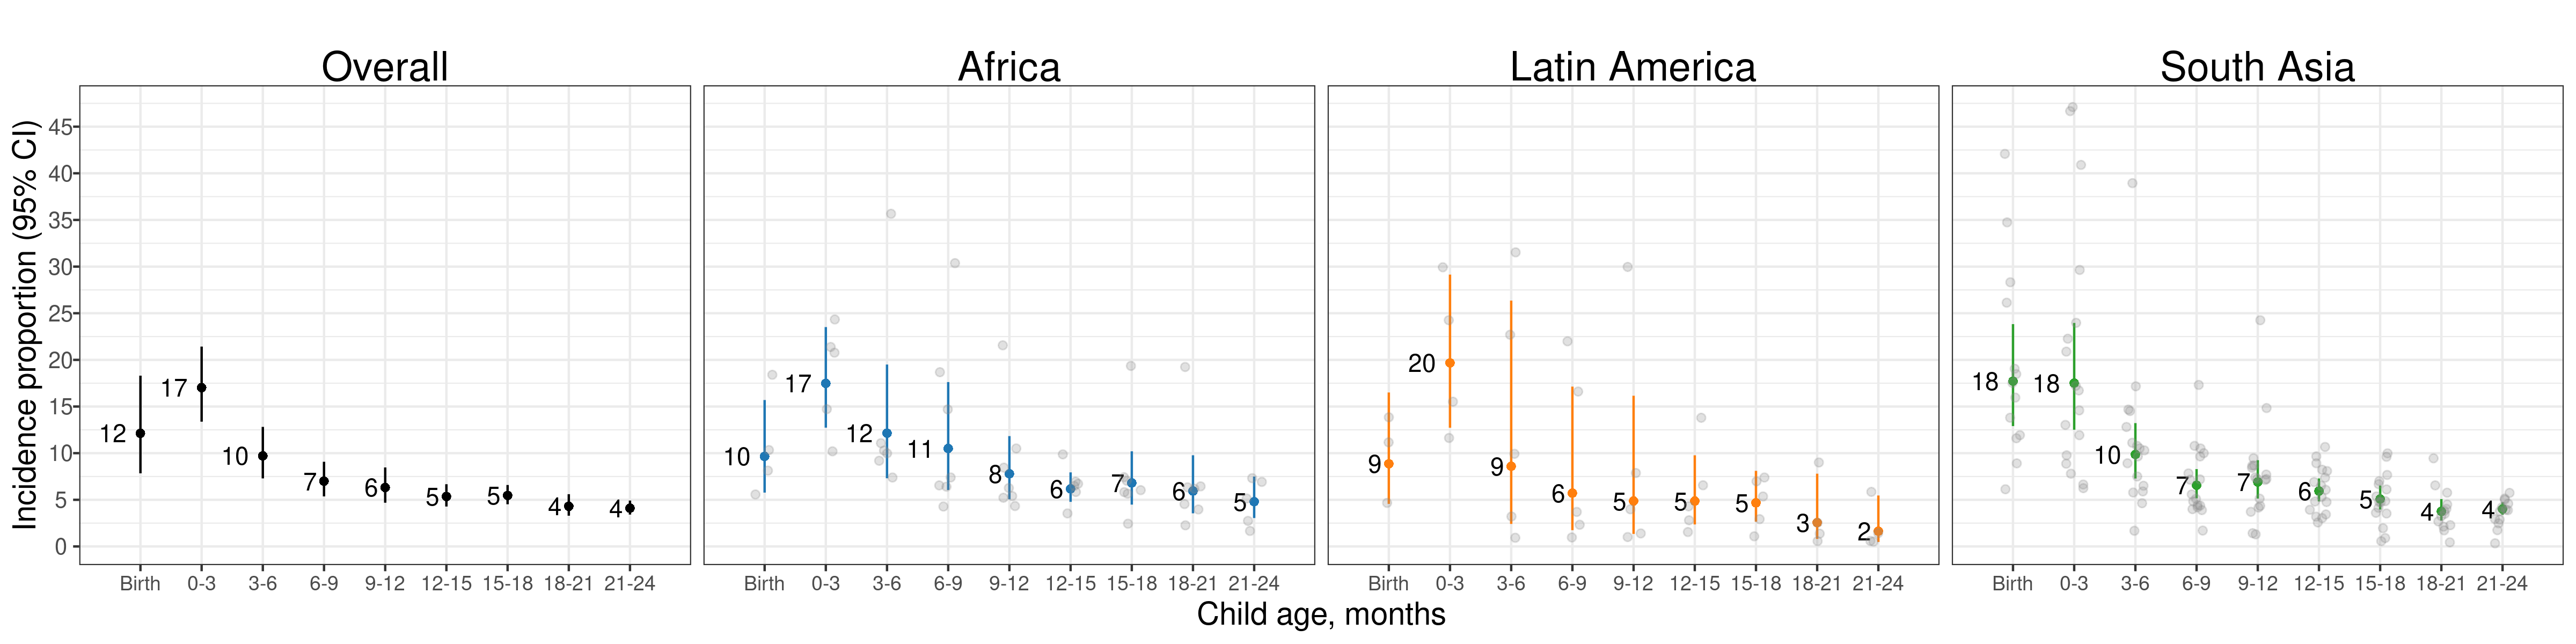
\includegraphics[width=66.67in]{figures//stunting/fig-stunt-2-inc-overall_region--allage-primary}

\hypertarget{cohorts-that-measured-monthly-from-birth-to-24-months-2}{%
\subsection{Cohorts that measured monthly from birth to 24 months}\label{cohorts-that-measured-monthly-from-birth-to-24-months-2}}

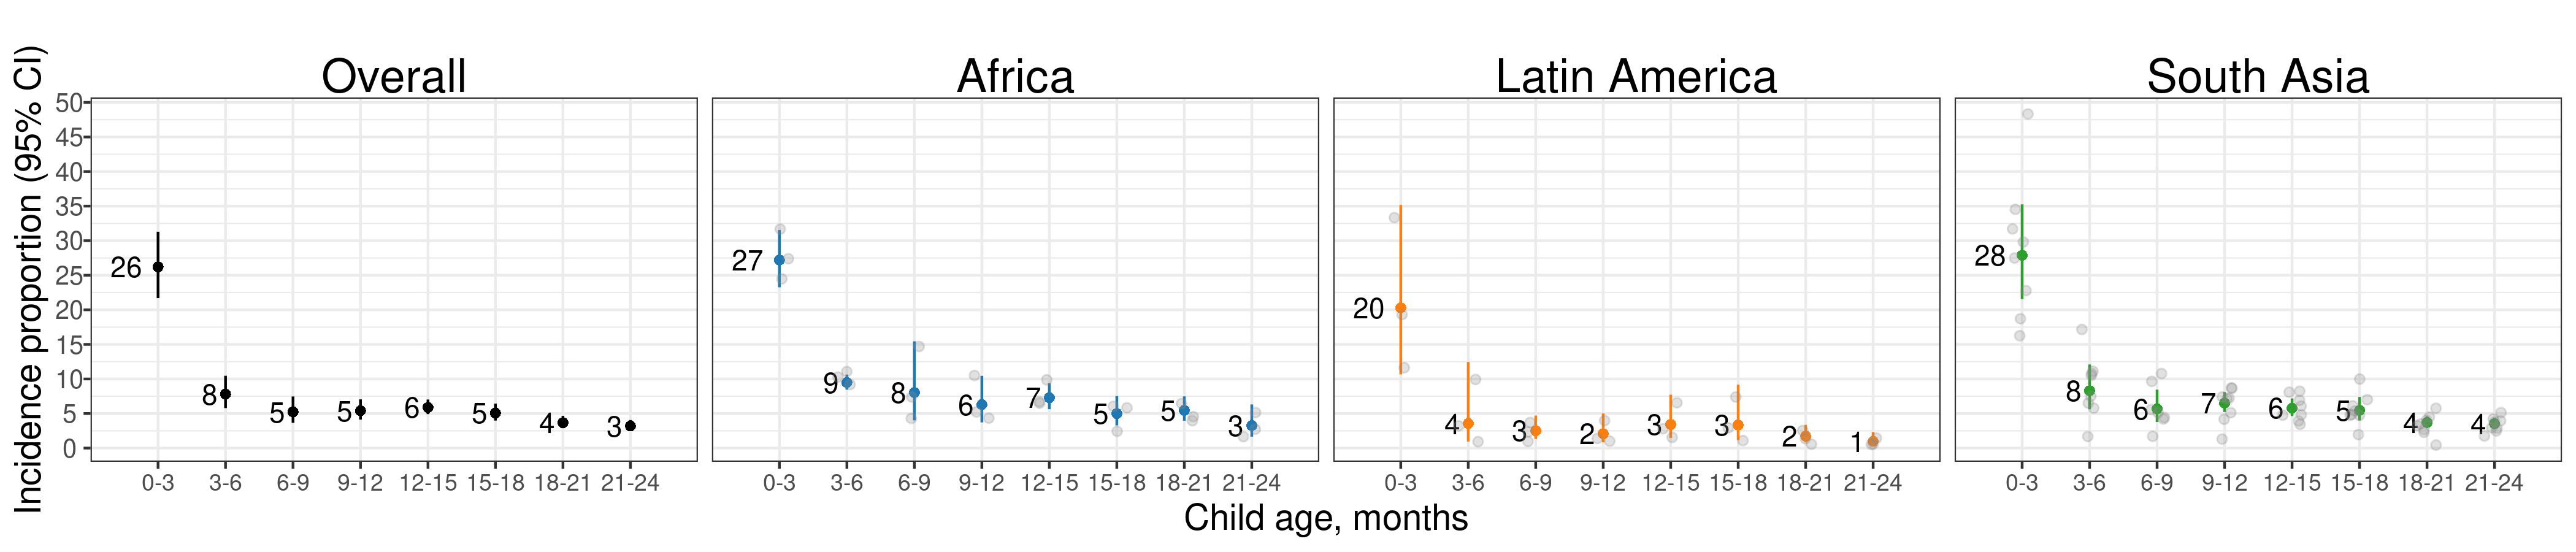
\includegraphics[width=58.33in]{figures//stunting/fig-stunt-2-inc-overall_region--allage-month24}

\hypertarget{linear-growth-velocity}{%
\section{Linear growth velocity}\label{linear-growth-velocity}}

\hypertarget{all-eligible-cohorts-3}{%
\subsection{All eligible cohorts}\label{all-eligible-cohorts-3}}

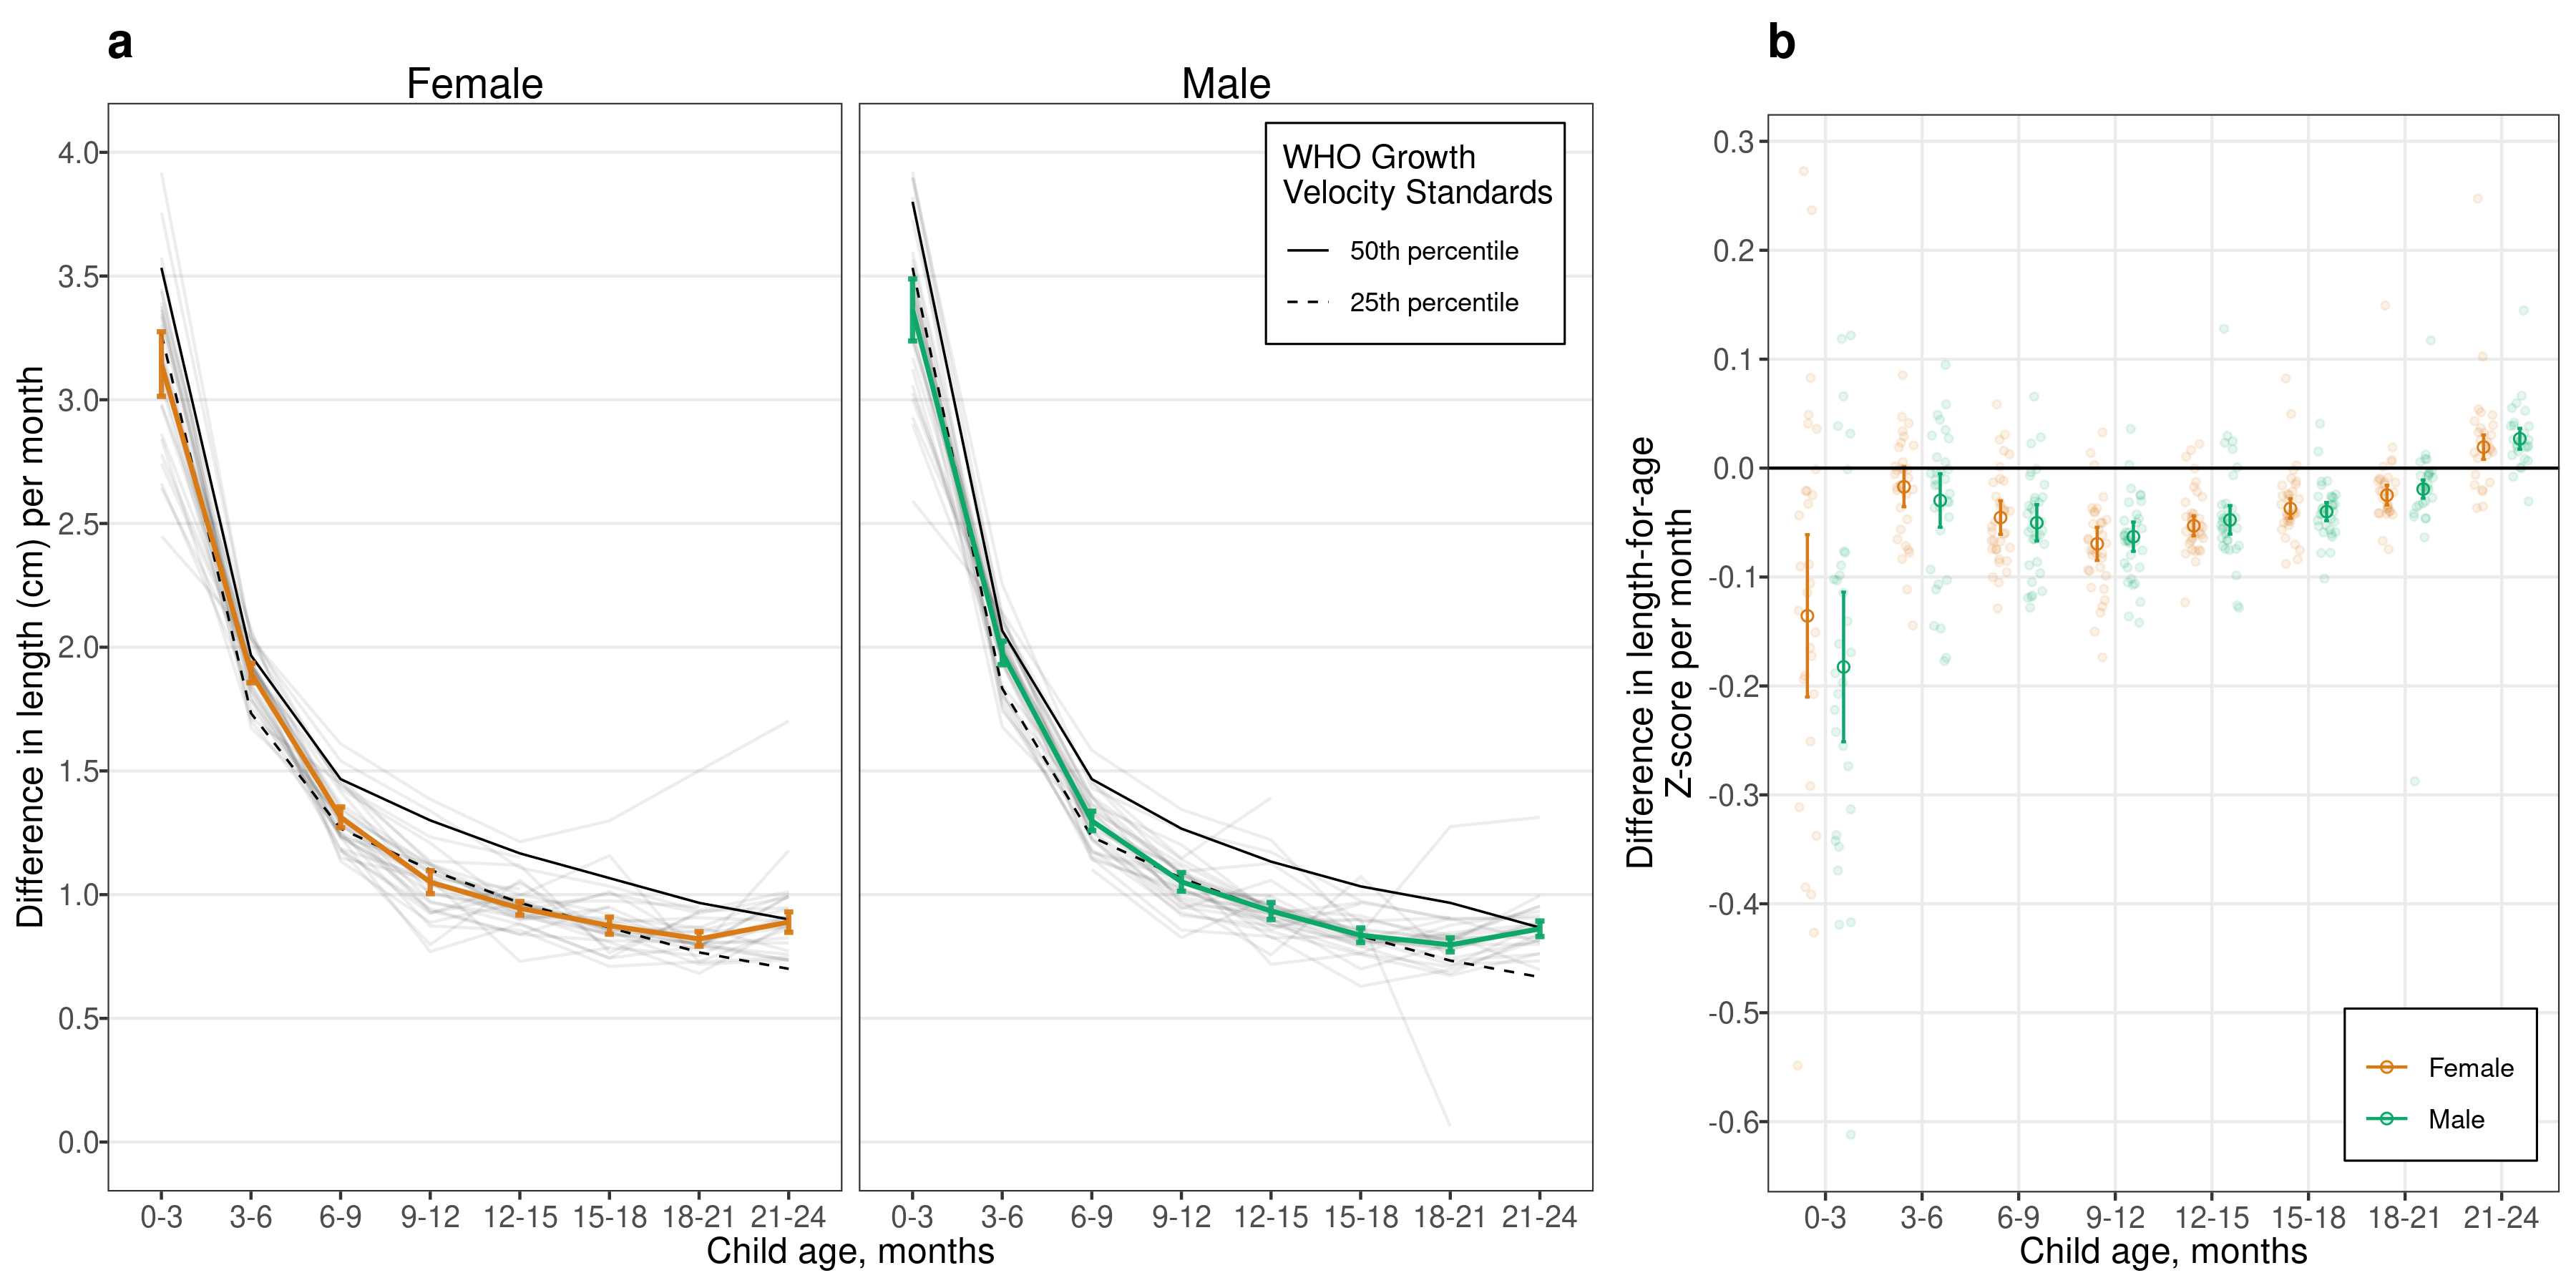
\includegraphics[width=50in]{figures//stunting/fig-stunt-2-vel-overall--allage-primary}

\hypertarget{cohorts-that-measured-monthly-from-birth-to-24-months-3}{%
\subsection{Cohorts that measured monthly from birth to 24 months}\label{cohorts-that-measured-monthly-from-birth-to-24-months-3}}

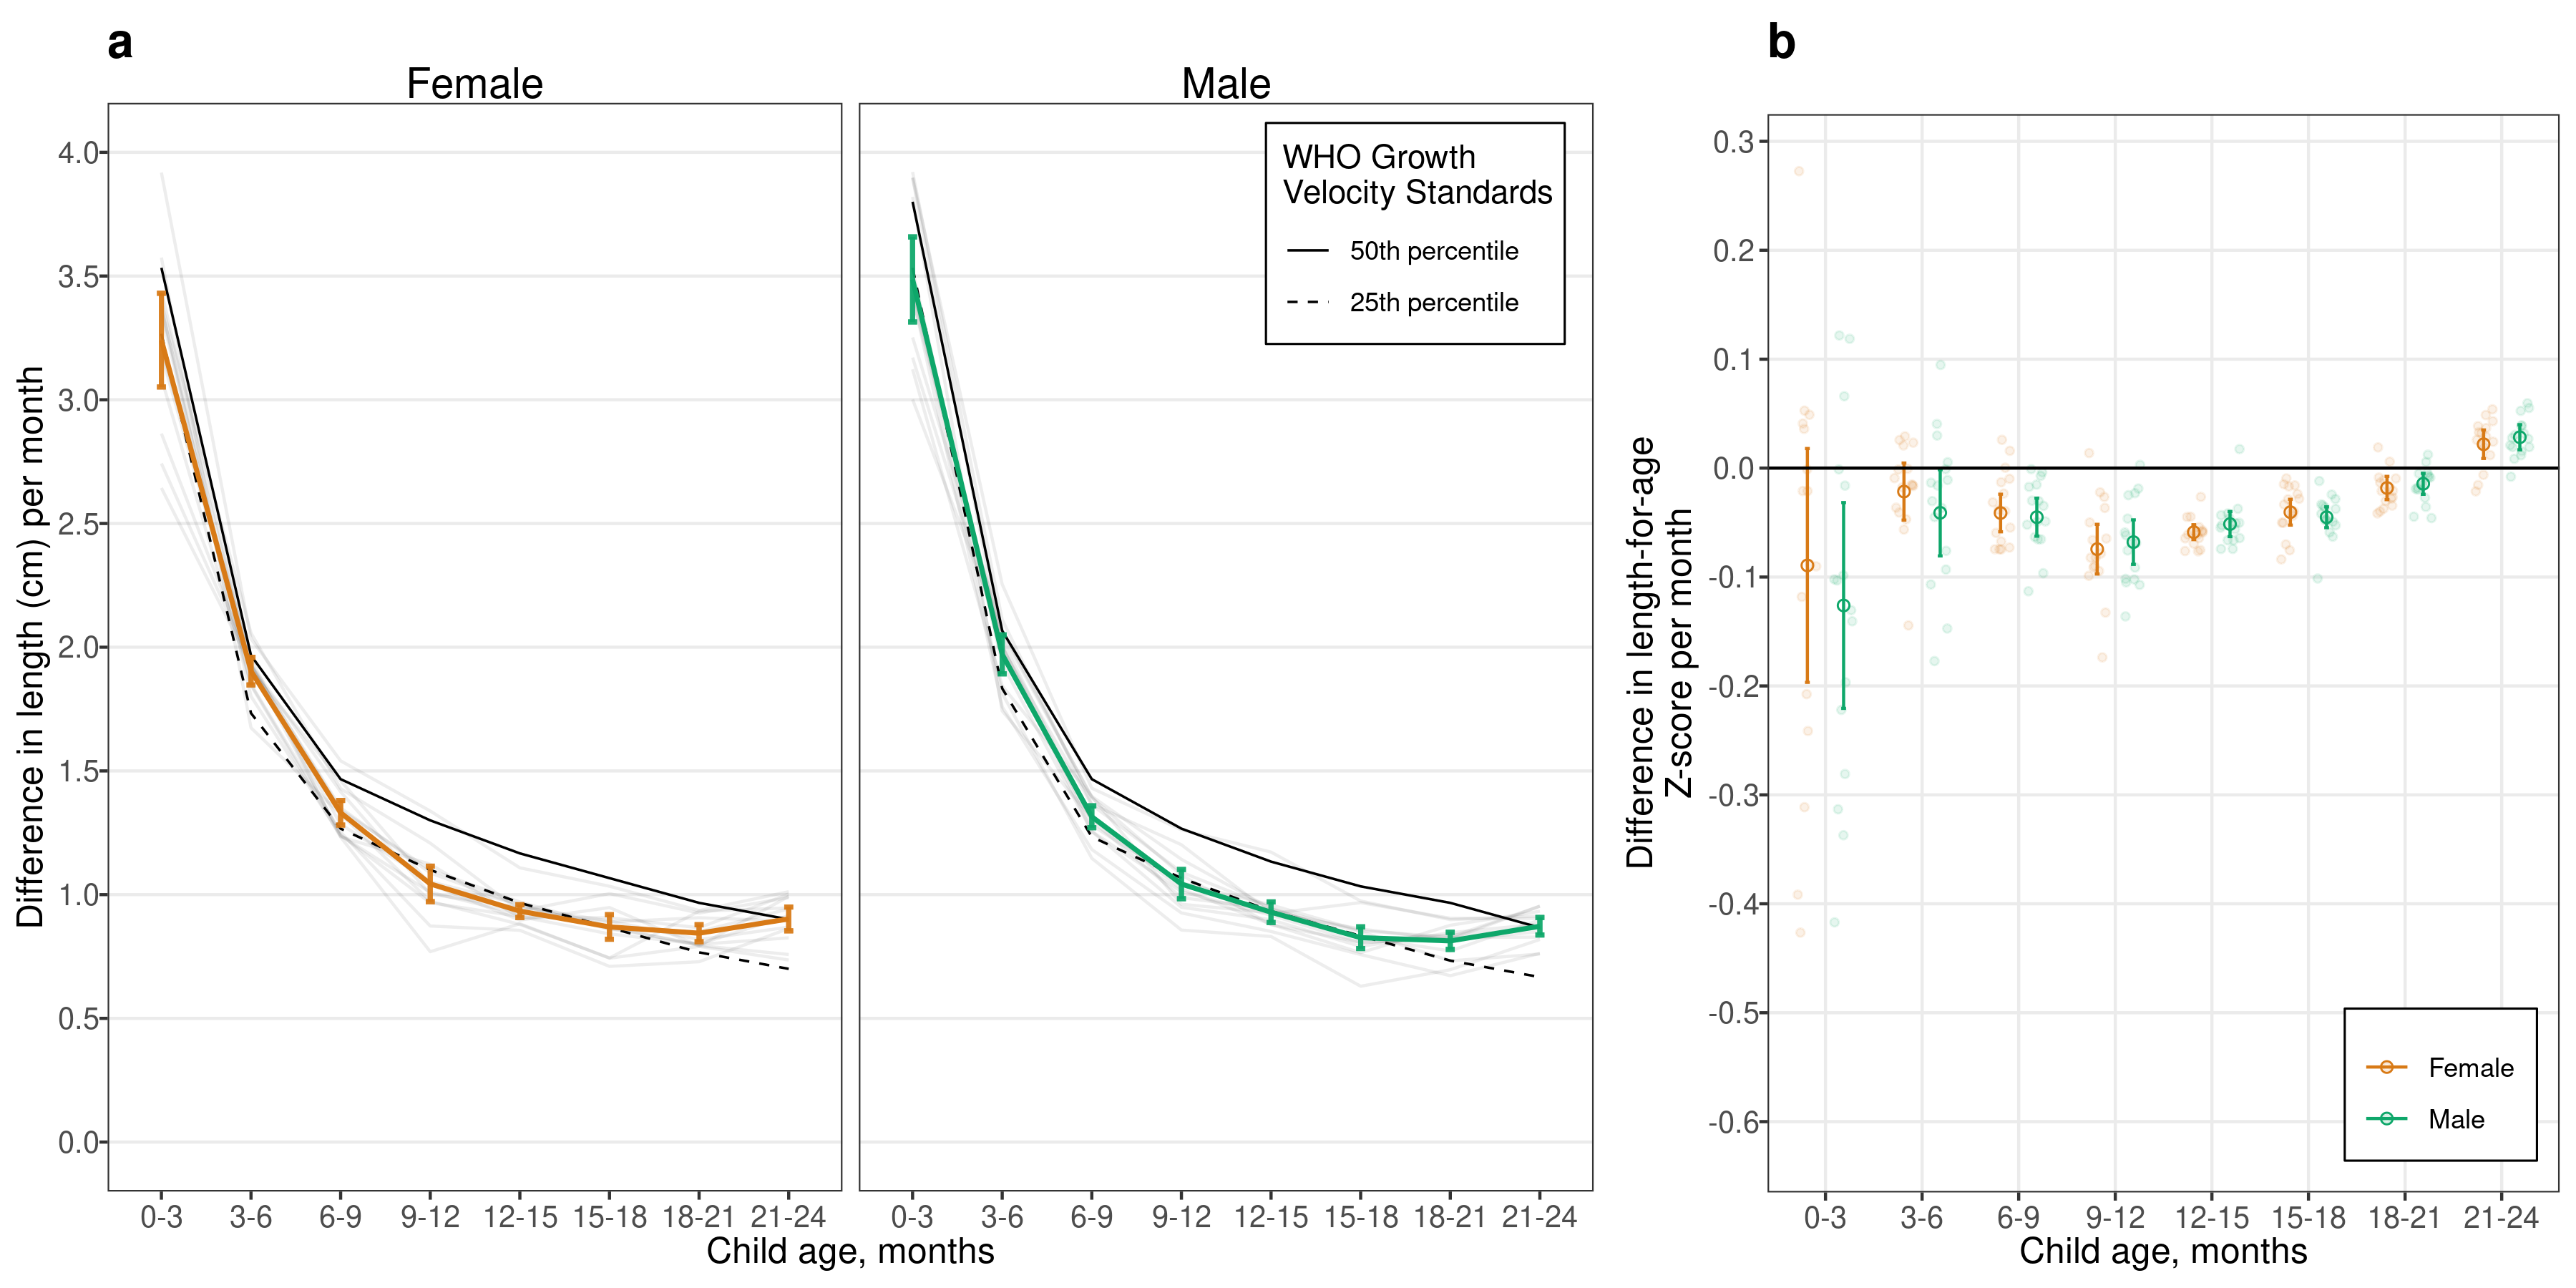
\includegraphics[width=41.67in]{figures//stunting/fig-stunt-2-vel-overall--allage-month24}

\hypertarget{fixed-effects}{%
\chapter{Sensitivity analysis using fixed effects}\label{fixed-effects}}

The primary analyses presented in this manuscript pooled across individual studies using random effects. Inferences about estimates from fixed effects models are restricted to only the included studies.\footnote{Hedges, L. V. \& Vevea, J. L. Fixed- and random-effects models in meta-analysis. Psychol. Methods 3, 486--504 (1998).} The random effects approach was more conservative in the presence of study heterogeneity, as evidenced by larger confidence intervals around each point estimates. Overall, the inference from results produced by each method was similar.

\hypertarget{age-specific-prevalence-2}{%
\section{Age-specific prevalence}\label{age-specific-prevalence-2}}

\hypertarget{random-effects}{%
\subsection{Random effects}\label{random-effects}}

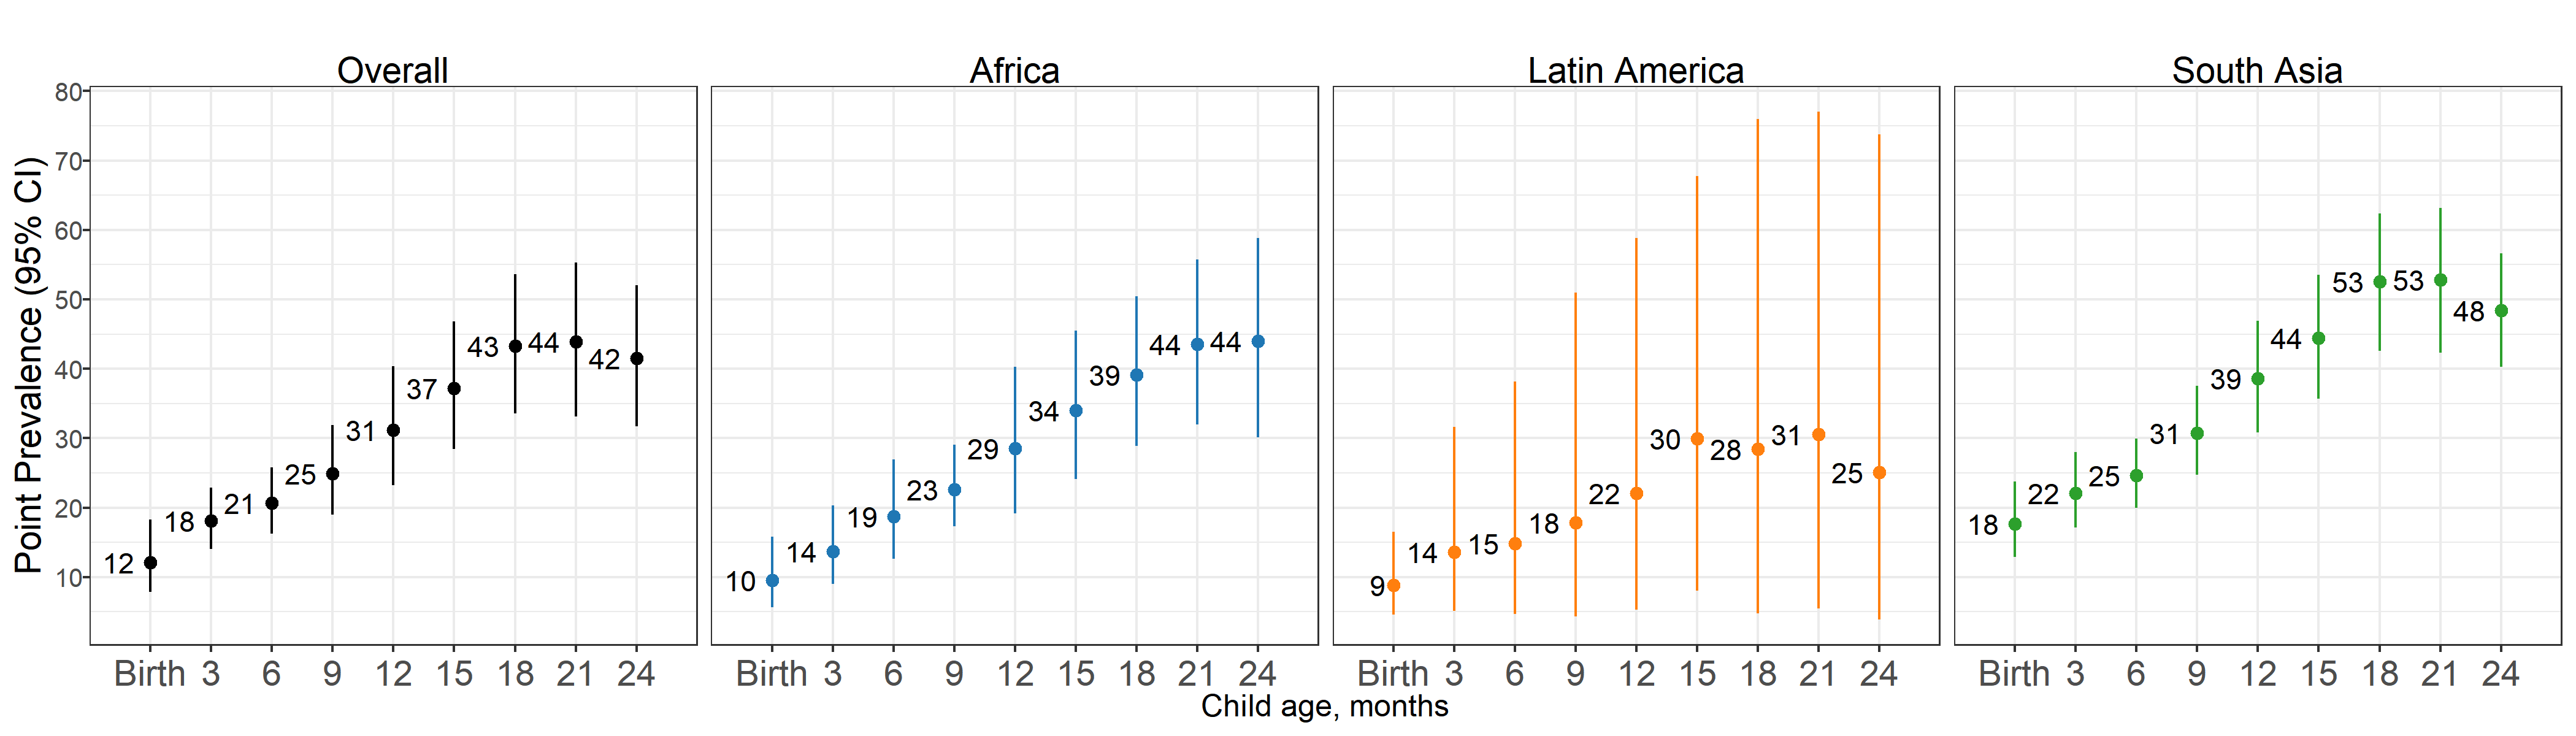
\includegraphics[width=58.33in]{figures//stunting/fig-stunt-2-prev-overall_region--allage-primary}

\hypertarget{fixed-effects-1}{%
\subsection{Fixed effects}\label{fixed-effects-1}}

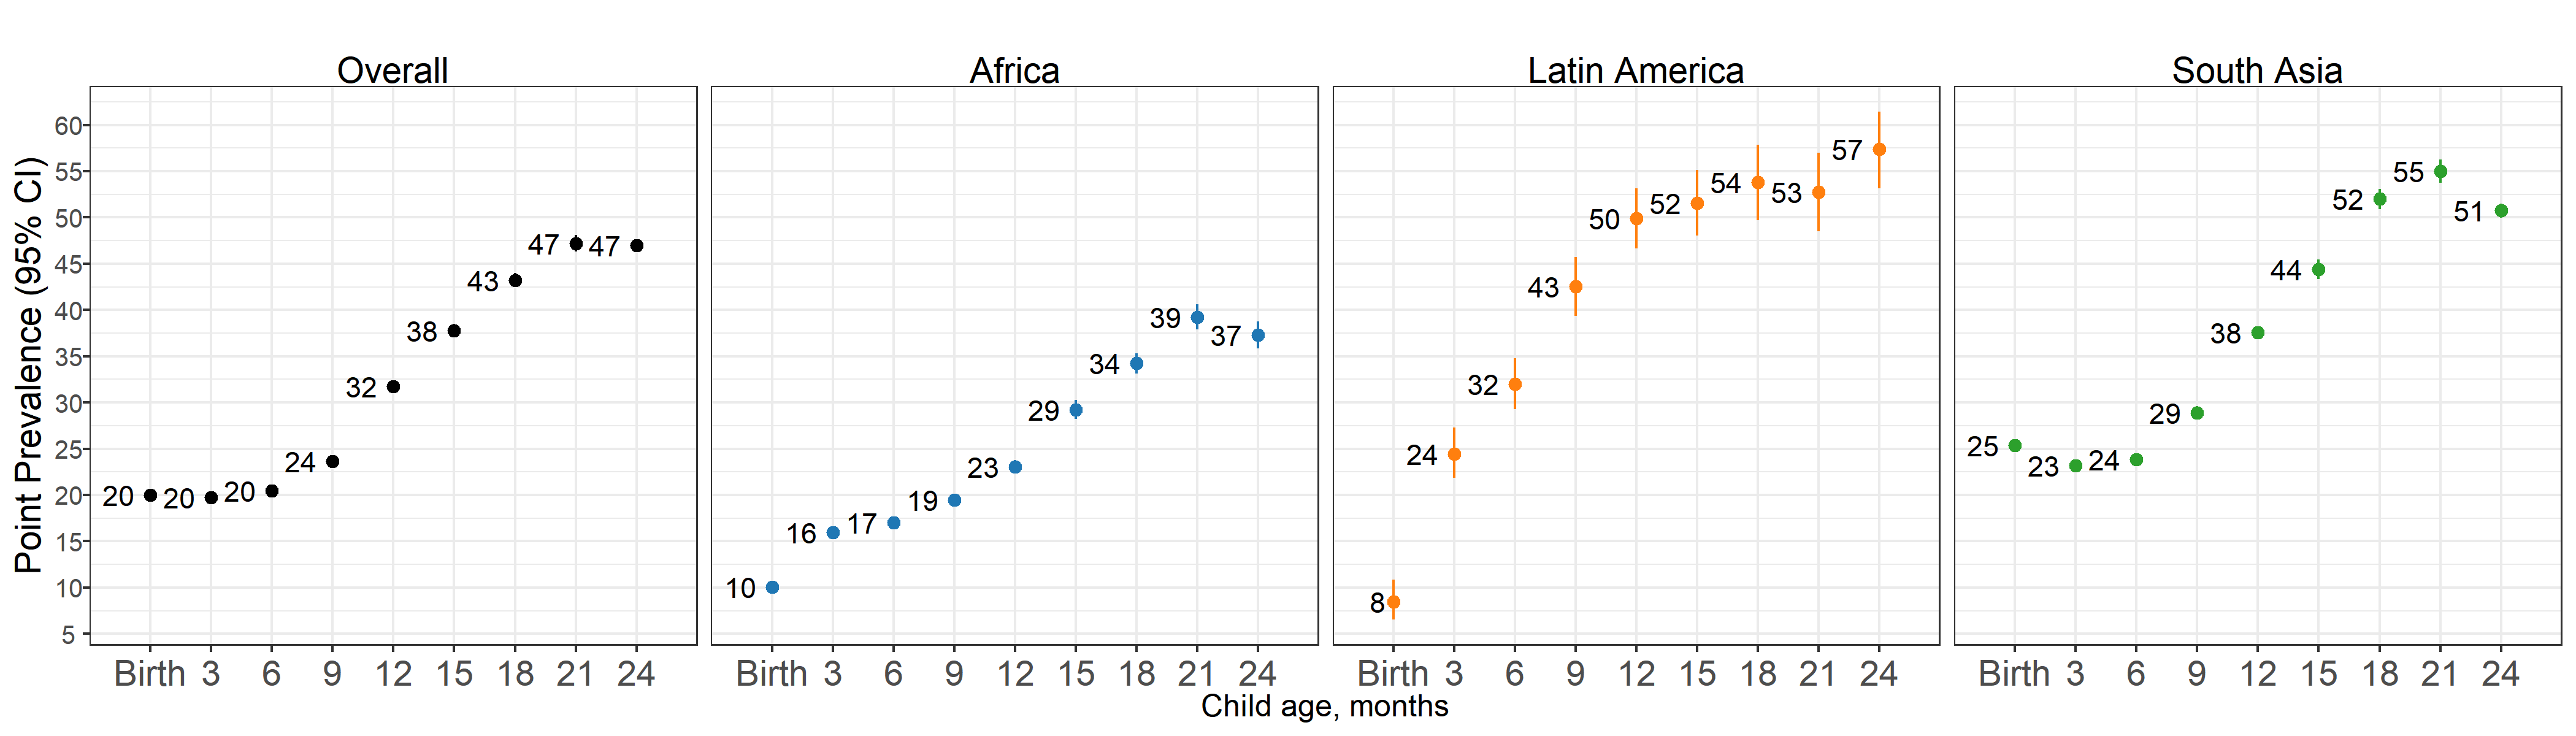
\includegraphics[width=58.33in]{figures//stunting/fig-stunt-2-prev-overall_region--allage-fe}

\hypertarget{age-specific-incidence-2}{%
\section{Age-specific incidence}\label{age-specific-incidence-2}}

\hypertarget{random-effects-1}{%
\subsection{Random effects}\label{random-effects-1}}

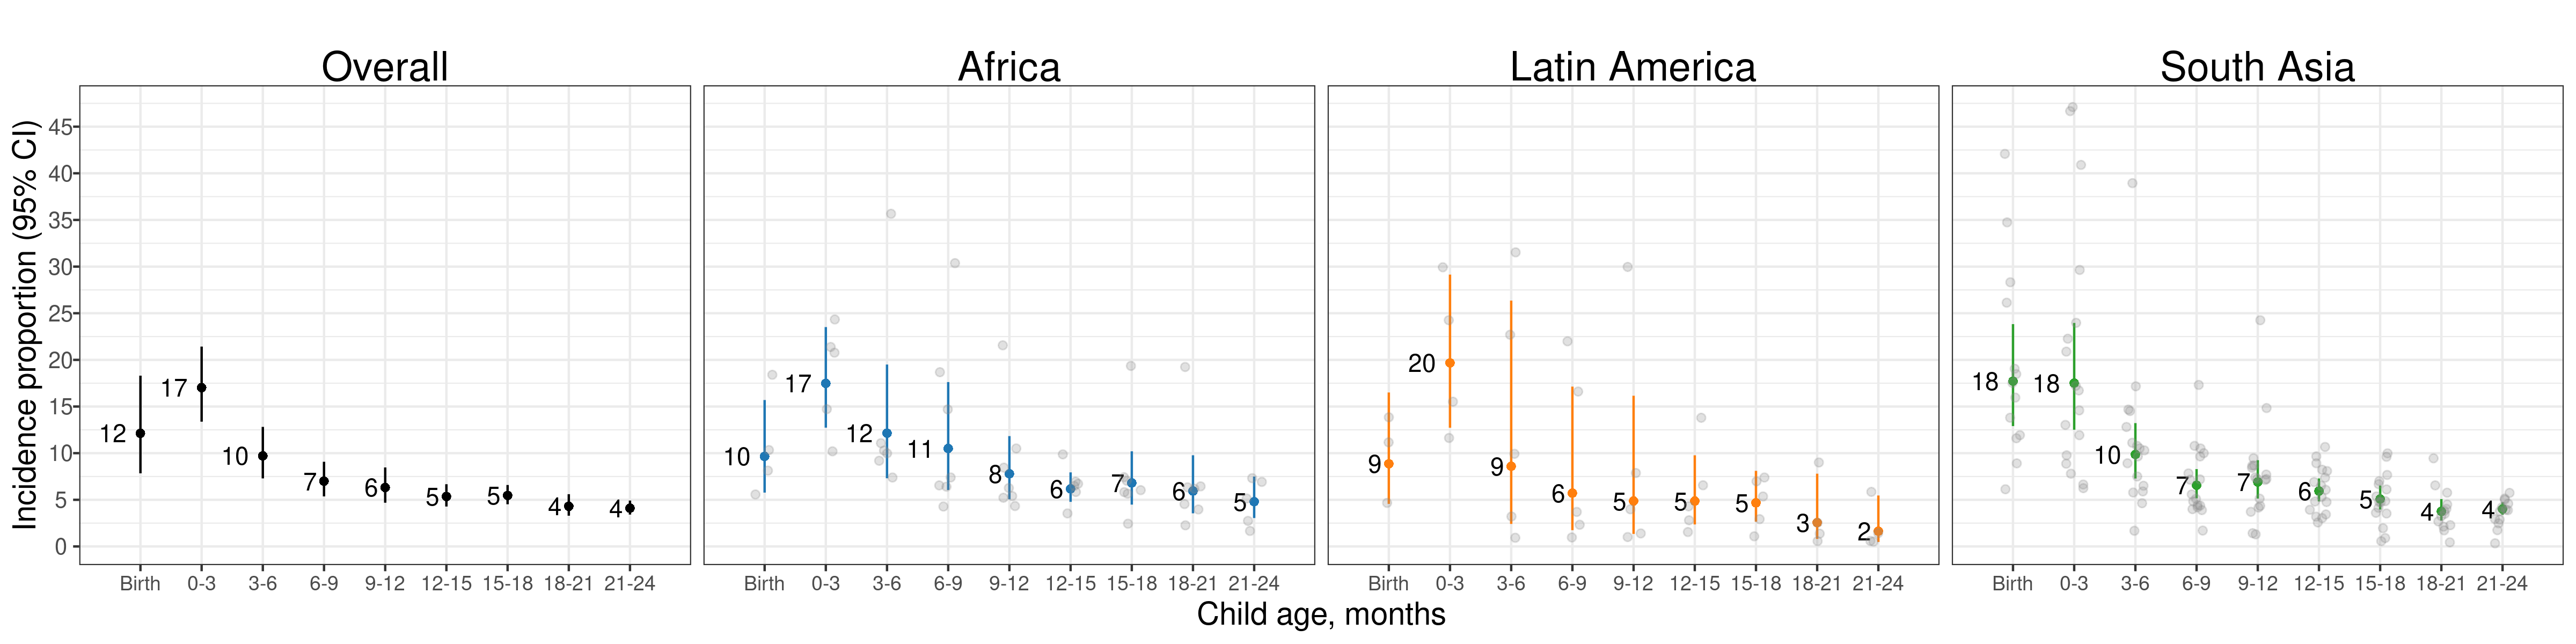
\includegraphics[width=66.67in]{figures//stunting/fig-stunt-2-inc-overall_region--allage-primary}

\hypertarget{fixed-effects-2}{%
\subsection{Fixed effects}\label{fixed-effects-2}}

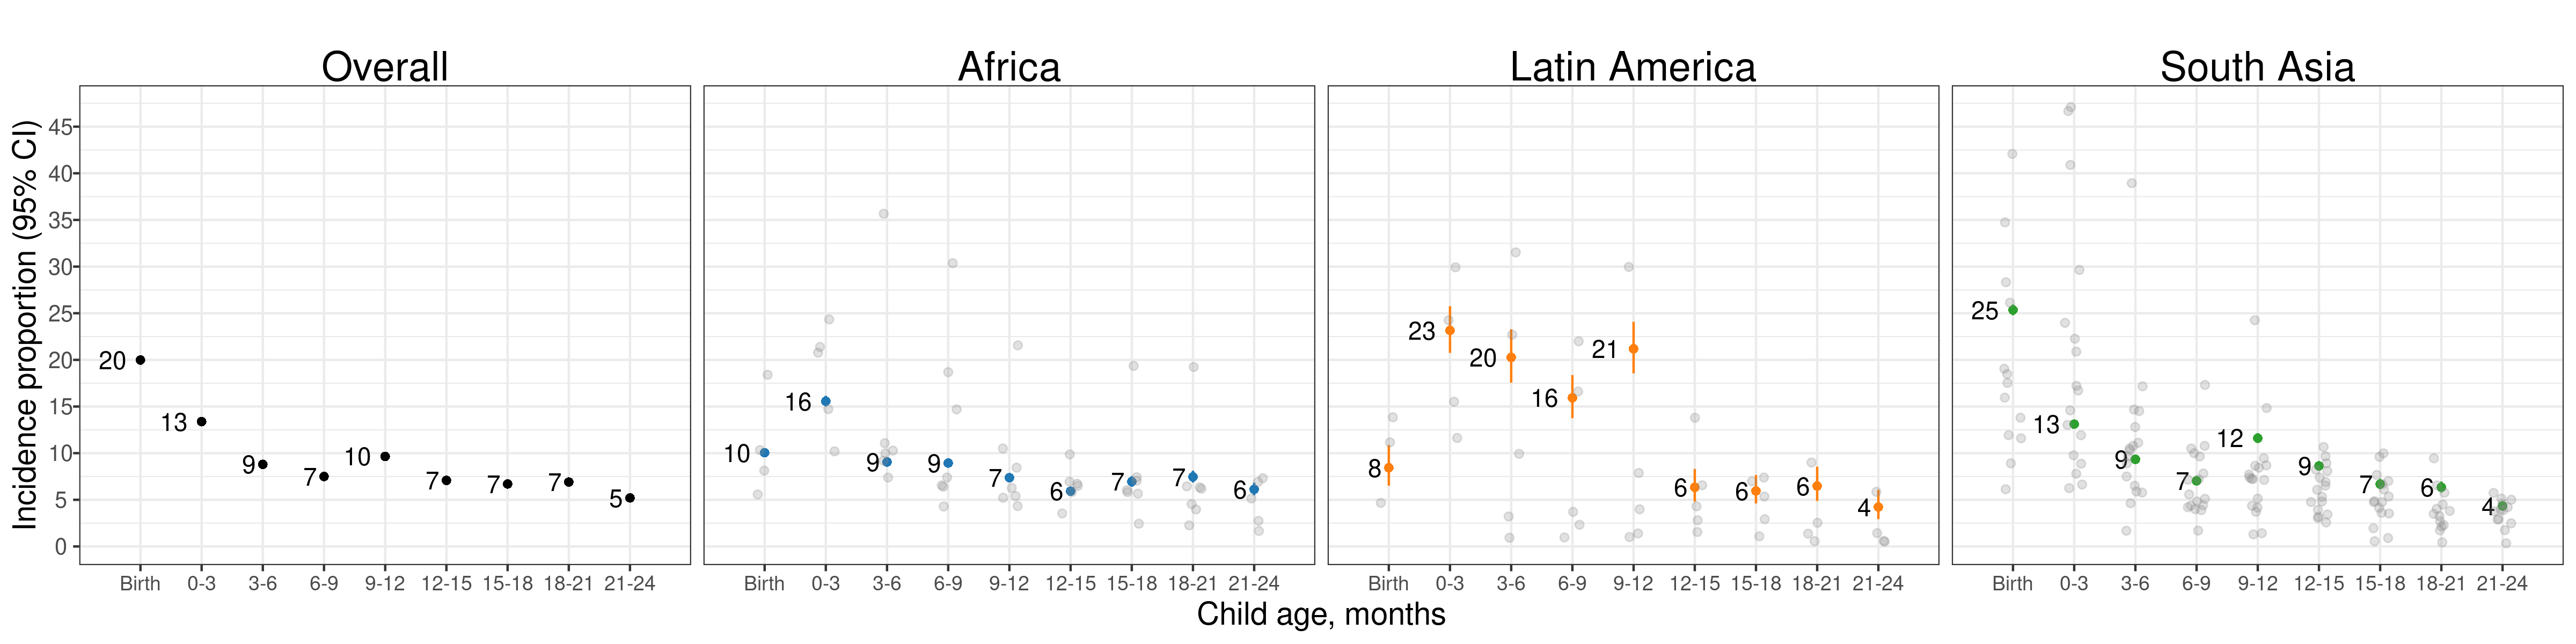
\includegraphics[width=66.67in]{figures//stunting/fig-stunt-2-inc-overall_region--allage-fe}

\hypertarget{changes-in-stunting-status-by-age}{%
\section{Changes in stunting status by age}\label{changes-in-stunting-status-by-age}}

\hypertarget{random-effects-2}{%
\subsection{Random effects}\label{random-effects-2}}

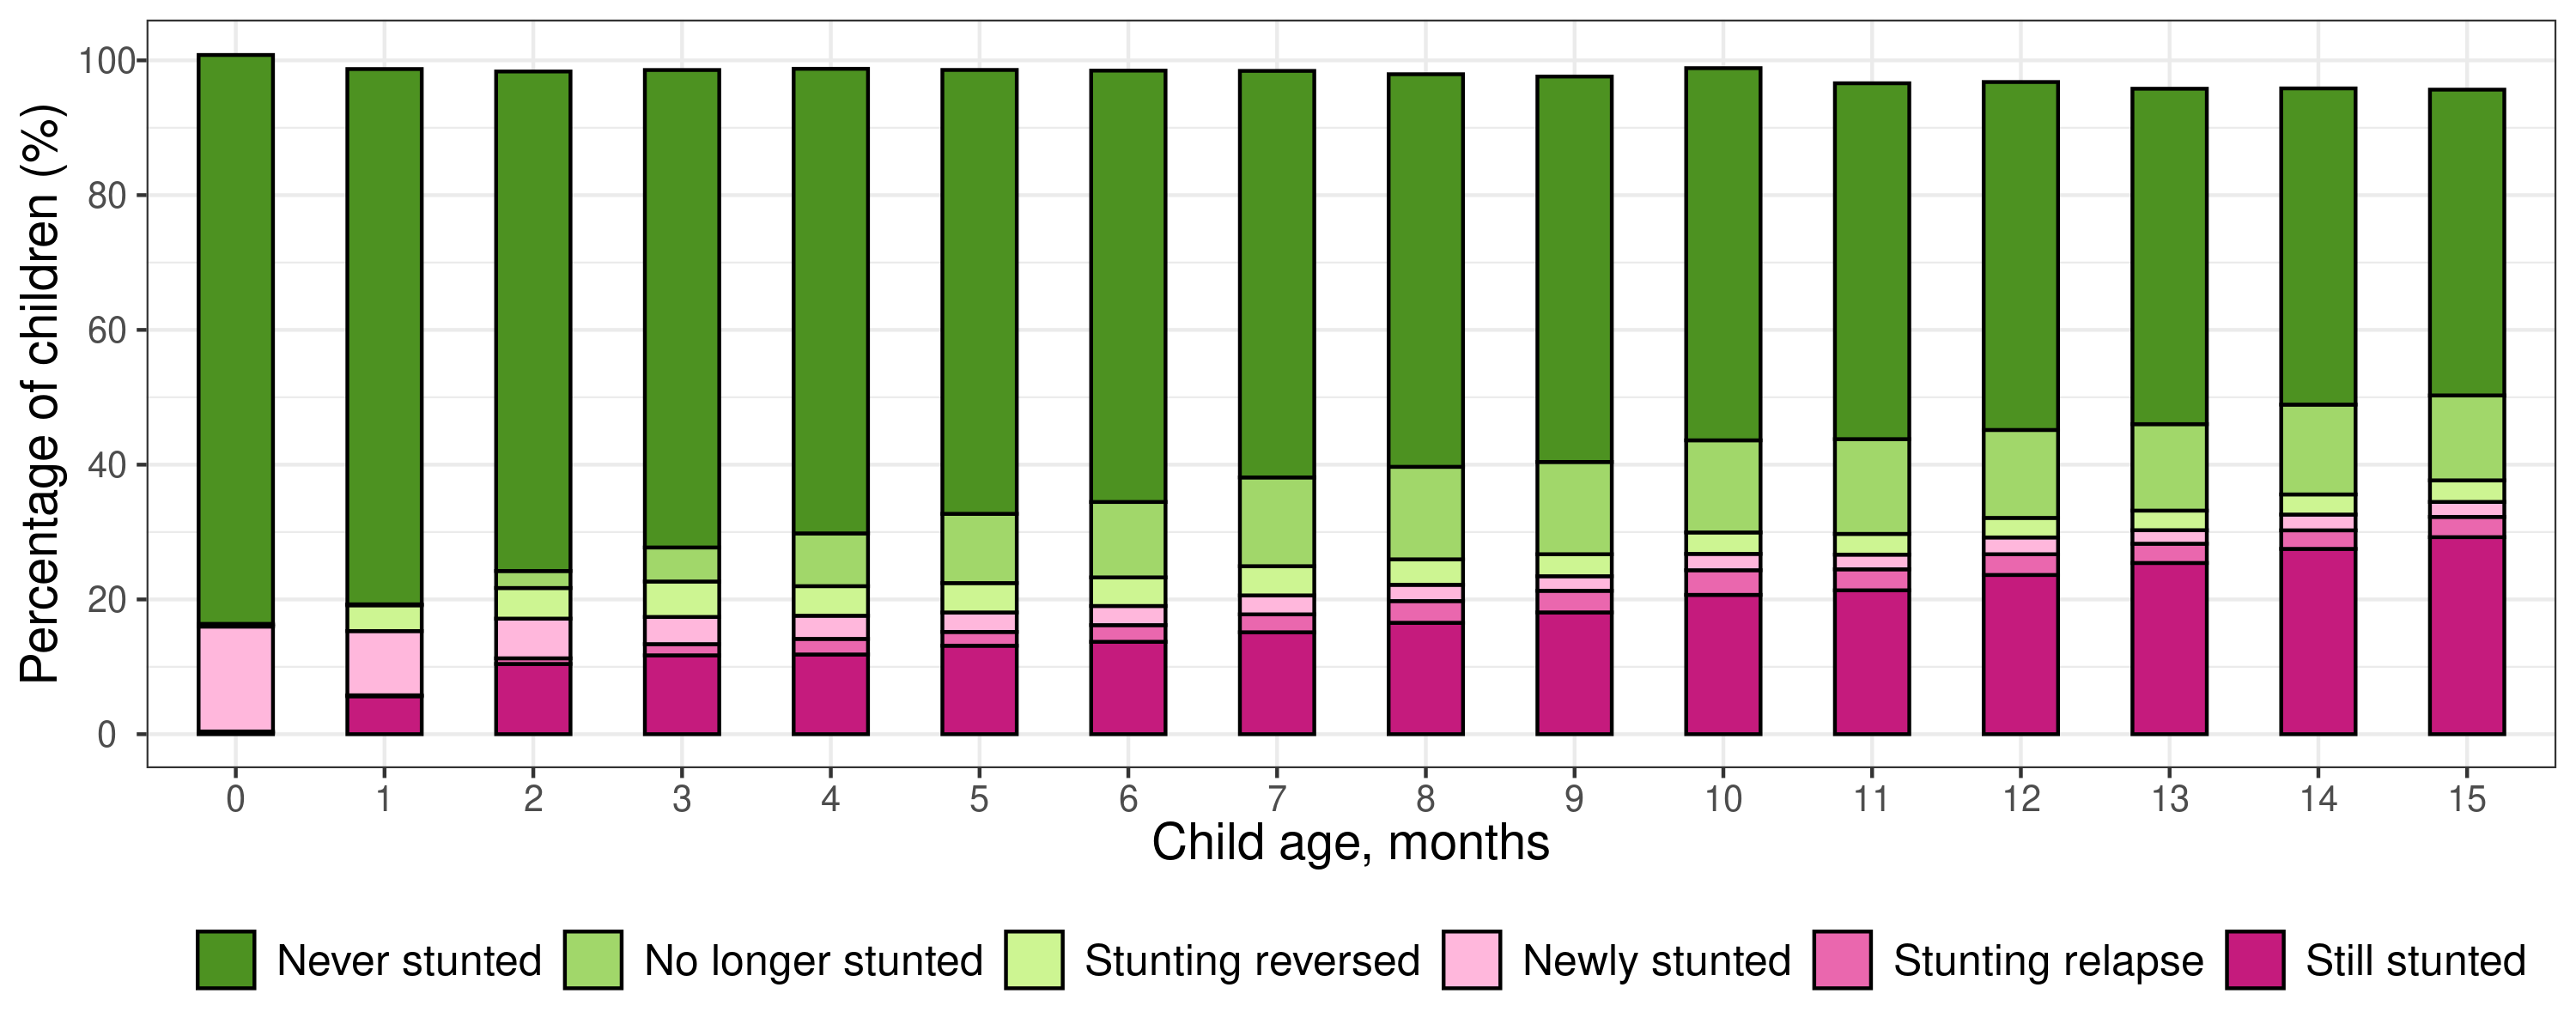
\includegraphics[width=41.67in]{figures//stunting/fig-stunt-2-flow-overall--allage-re}

\hypertarget{fixed-effects-3}{%
\subsection{Fixed effects}\label{fixed-effects-3}}

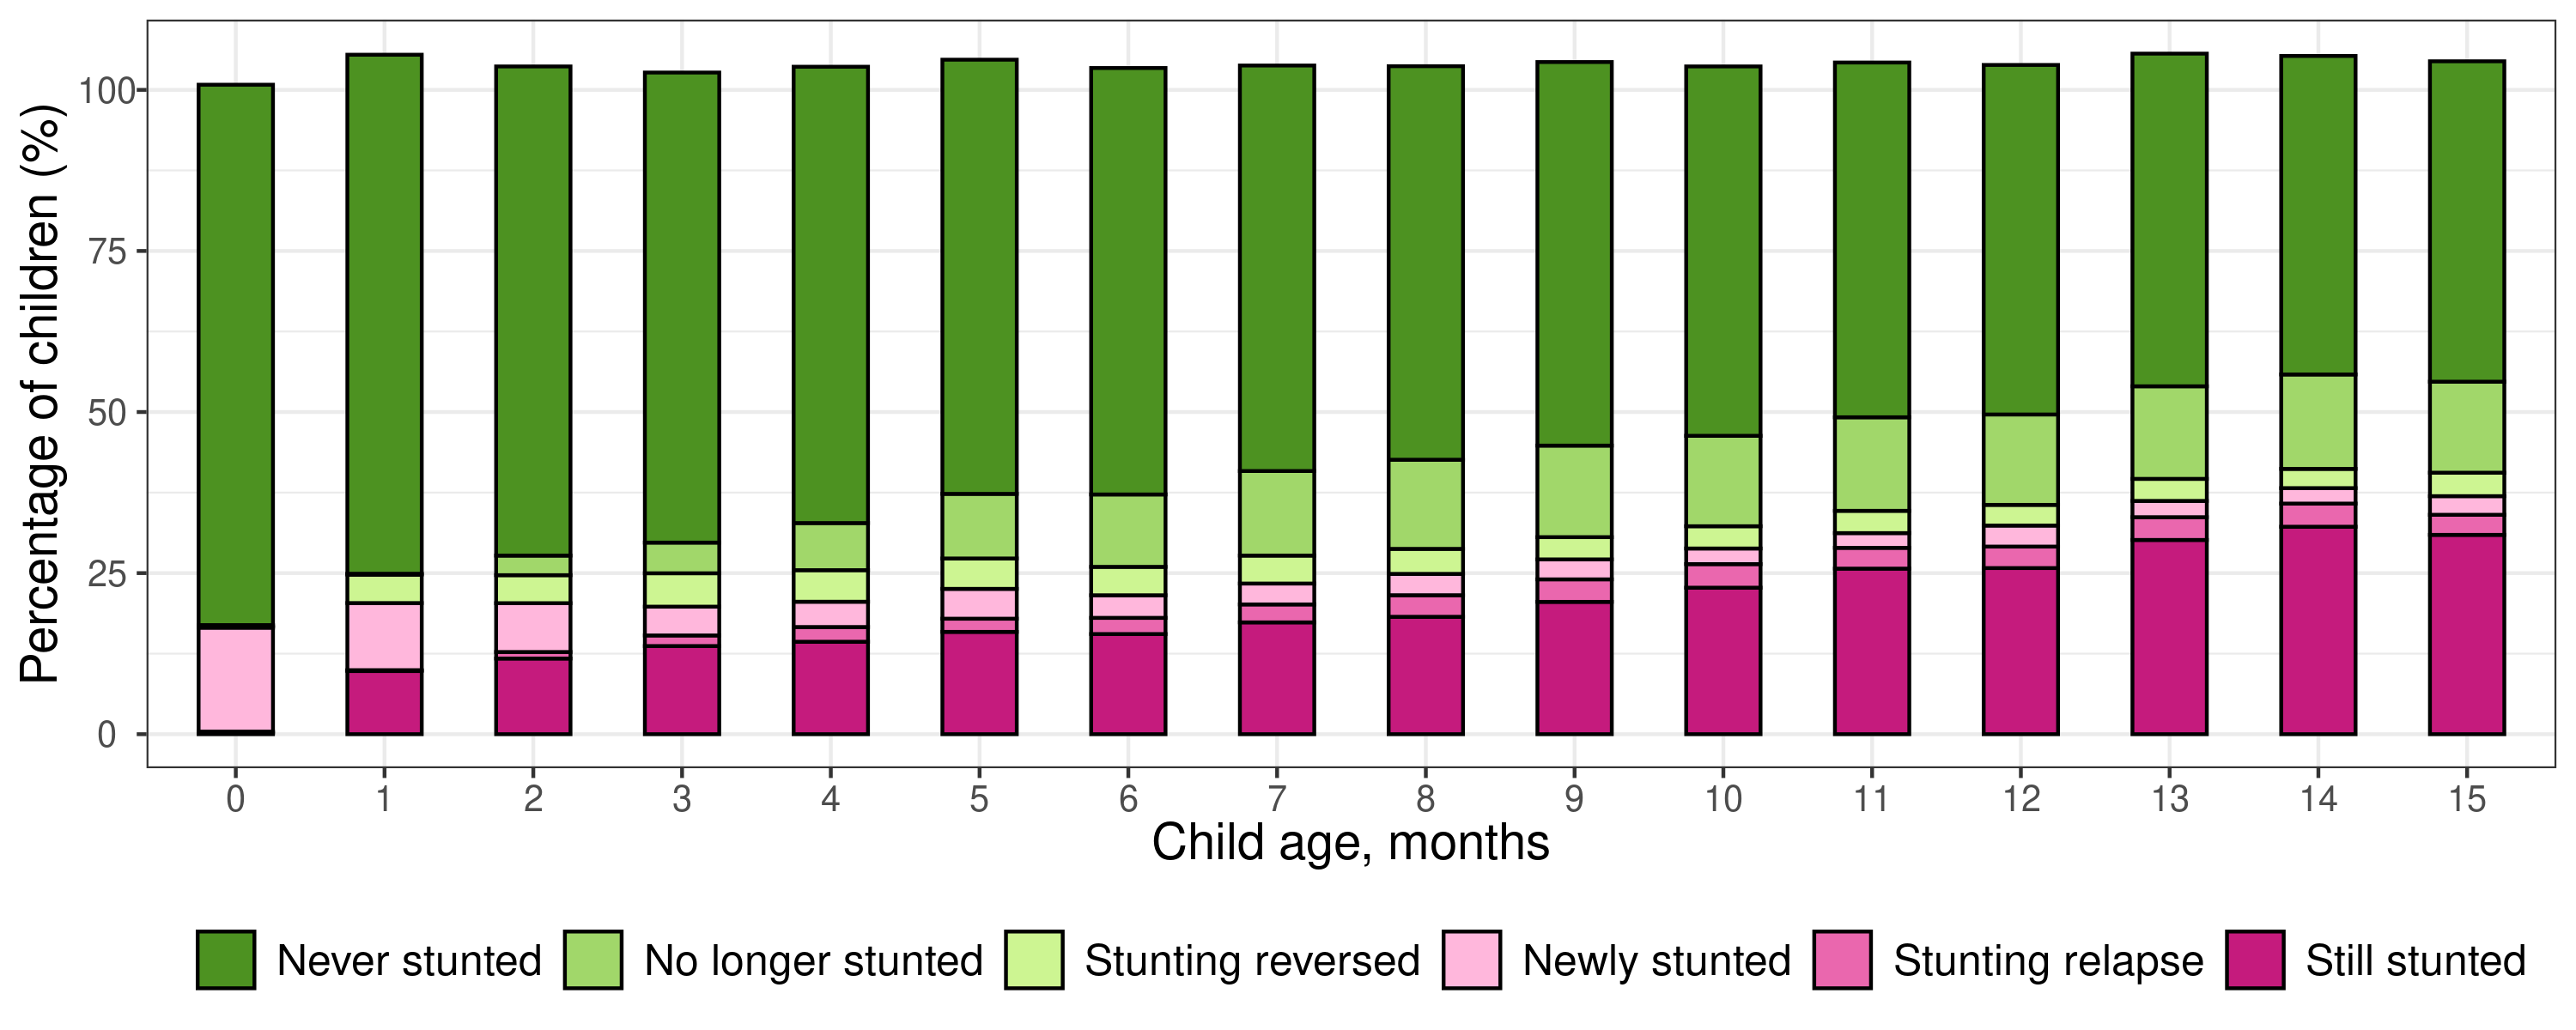
\includegraphics[width=41.67in]{figures//stunting/fig-stunt-2-flow-overall--allage-fe}

\hypertarget{linear-growth-velocity-1}{%
\section{Linear growth velocity}\label{linear-growth-velocity-1}}

\hypertarget{random-effects-3}{%
\subsection{Random effects}\label{random-effects-3}}

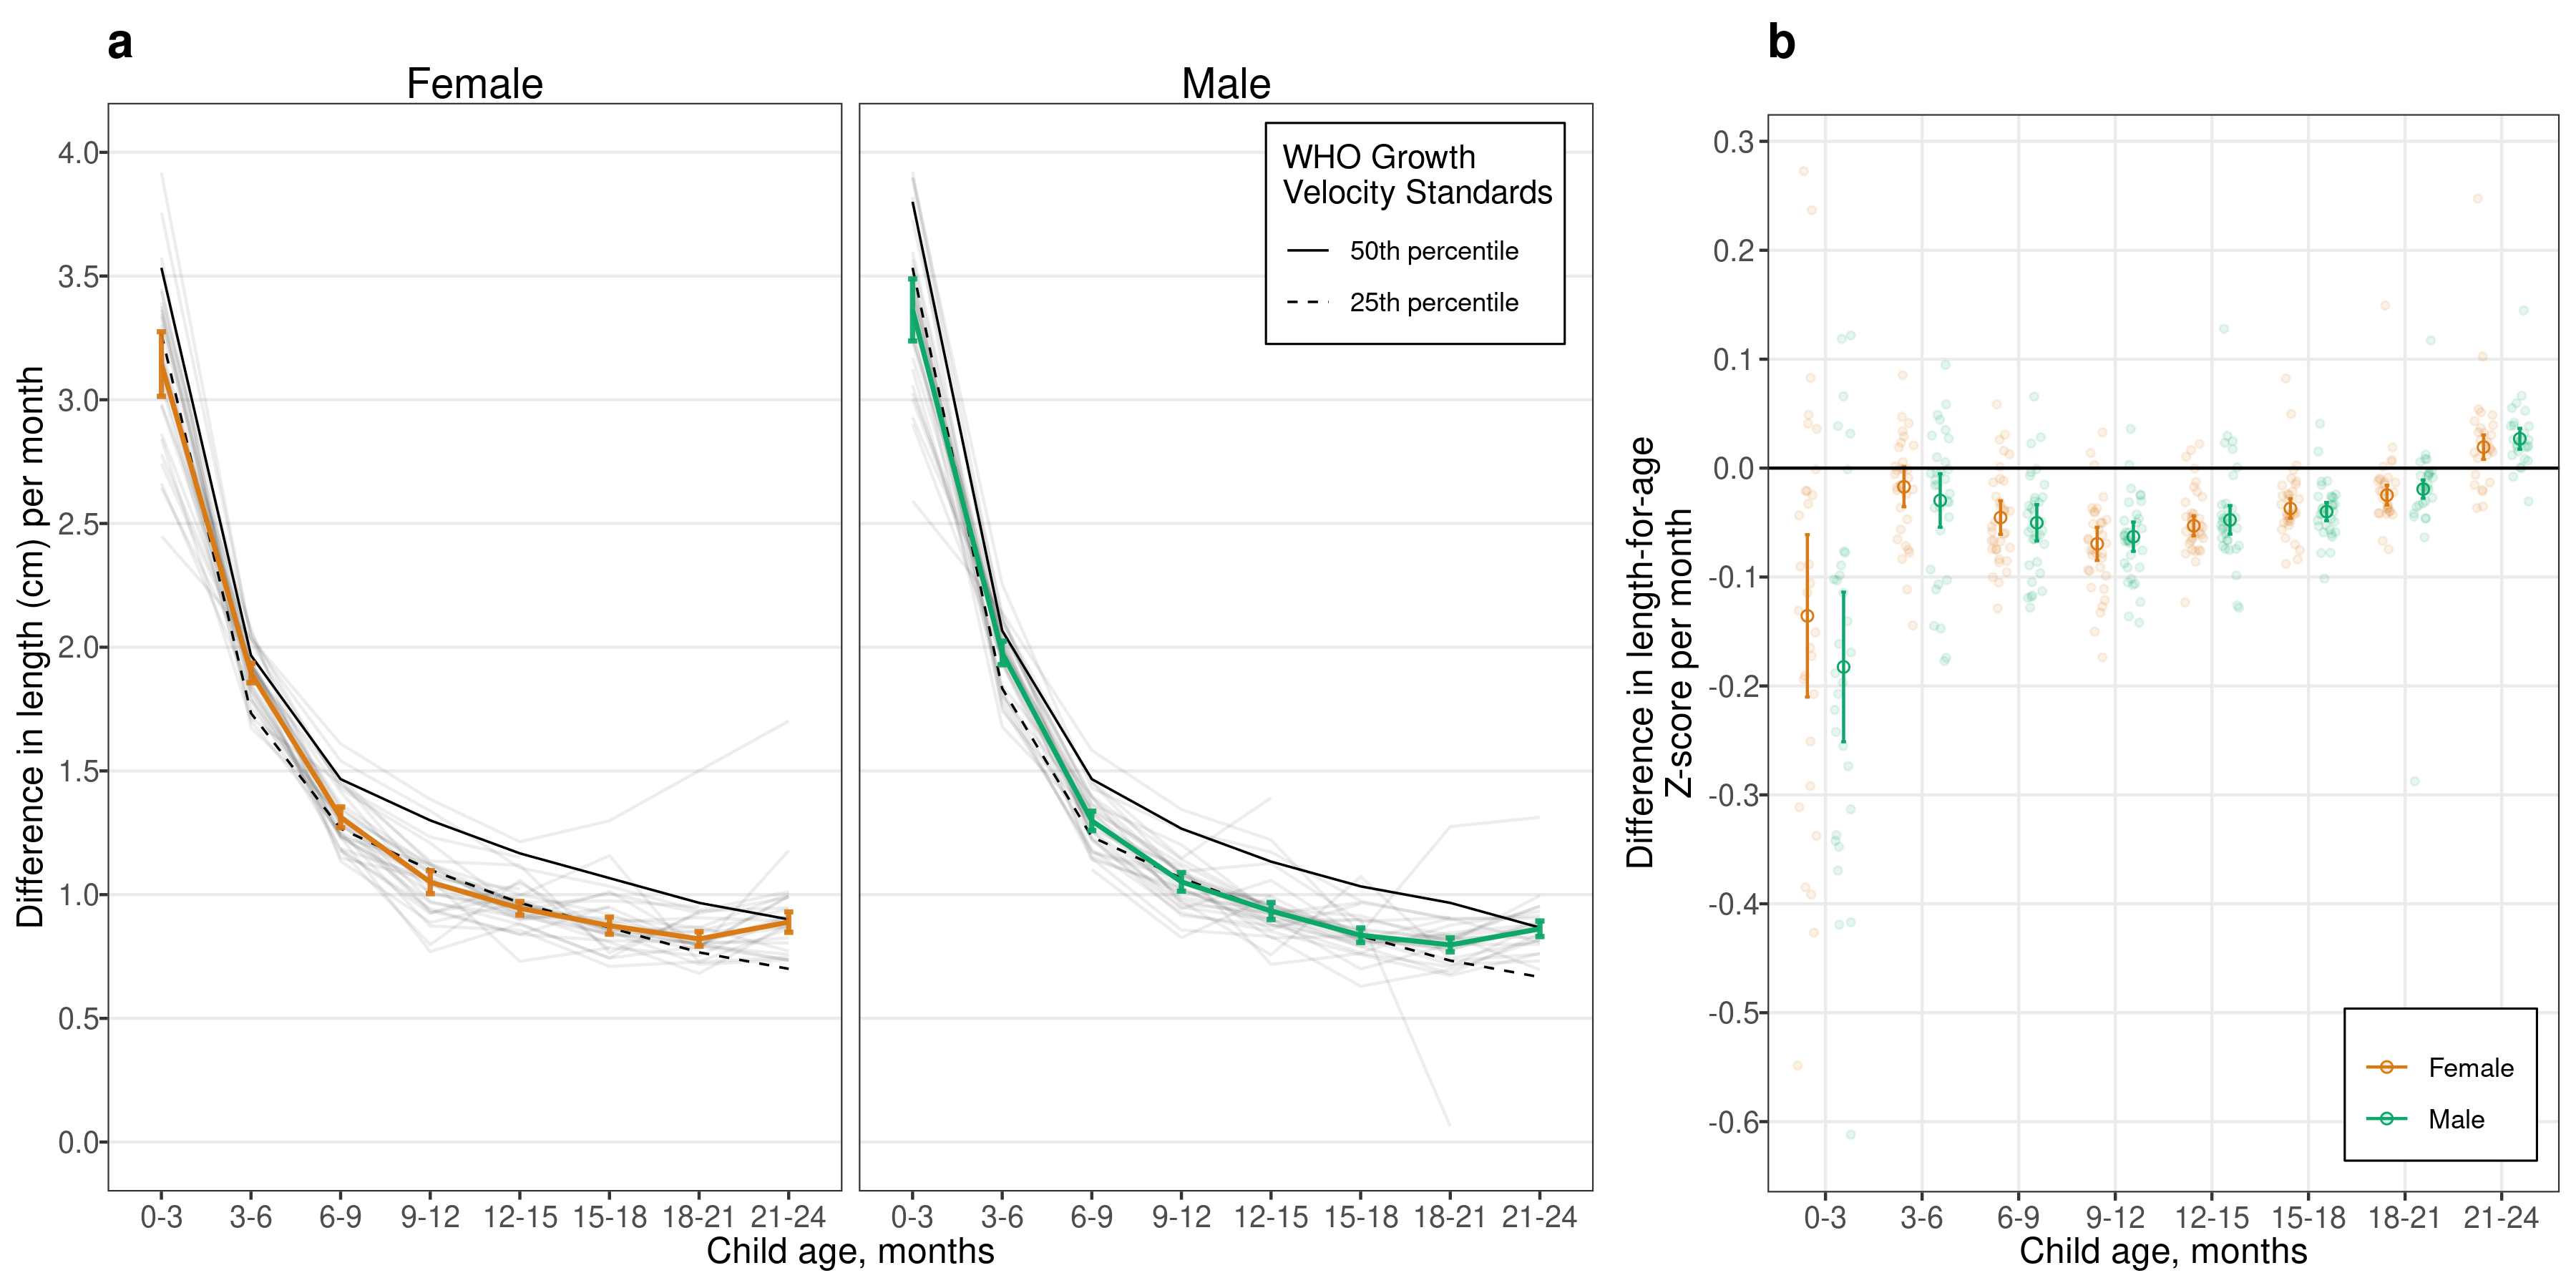
\includegraphics[width=50in]{figures//stunting/fig-stunt-2-vel-overall--allage-primary}

\hypertarget{fixed-effects-4}{%
\subsection{Fixed effects}\label{fixed-effects-4}}

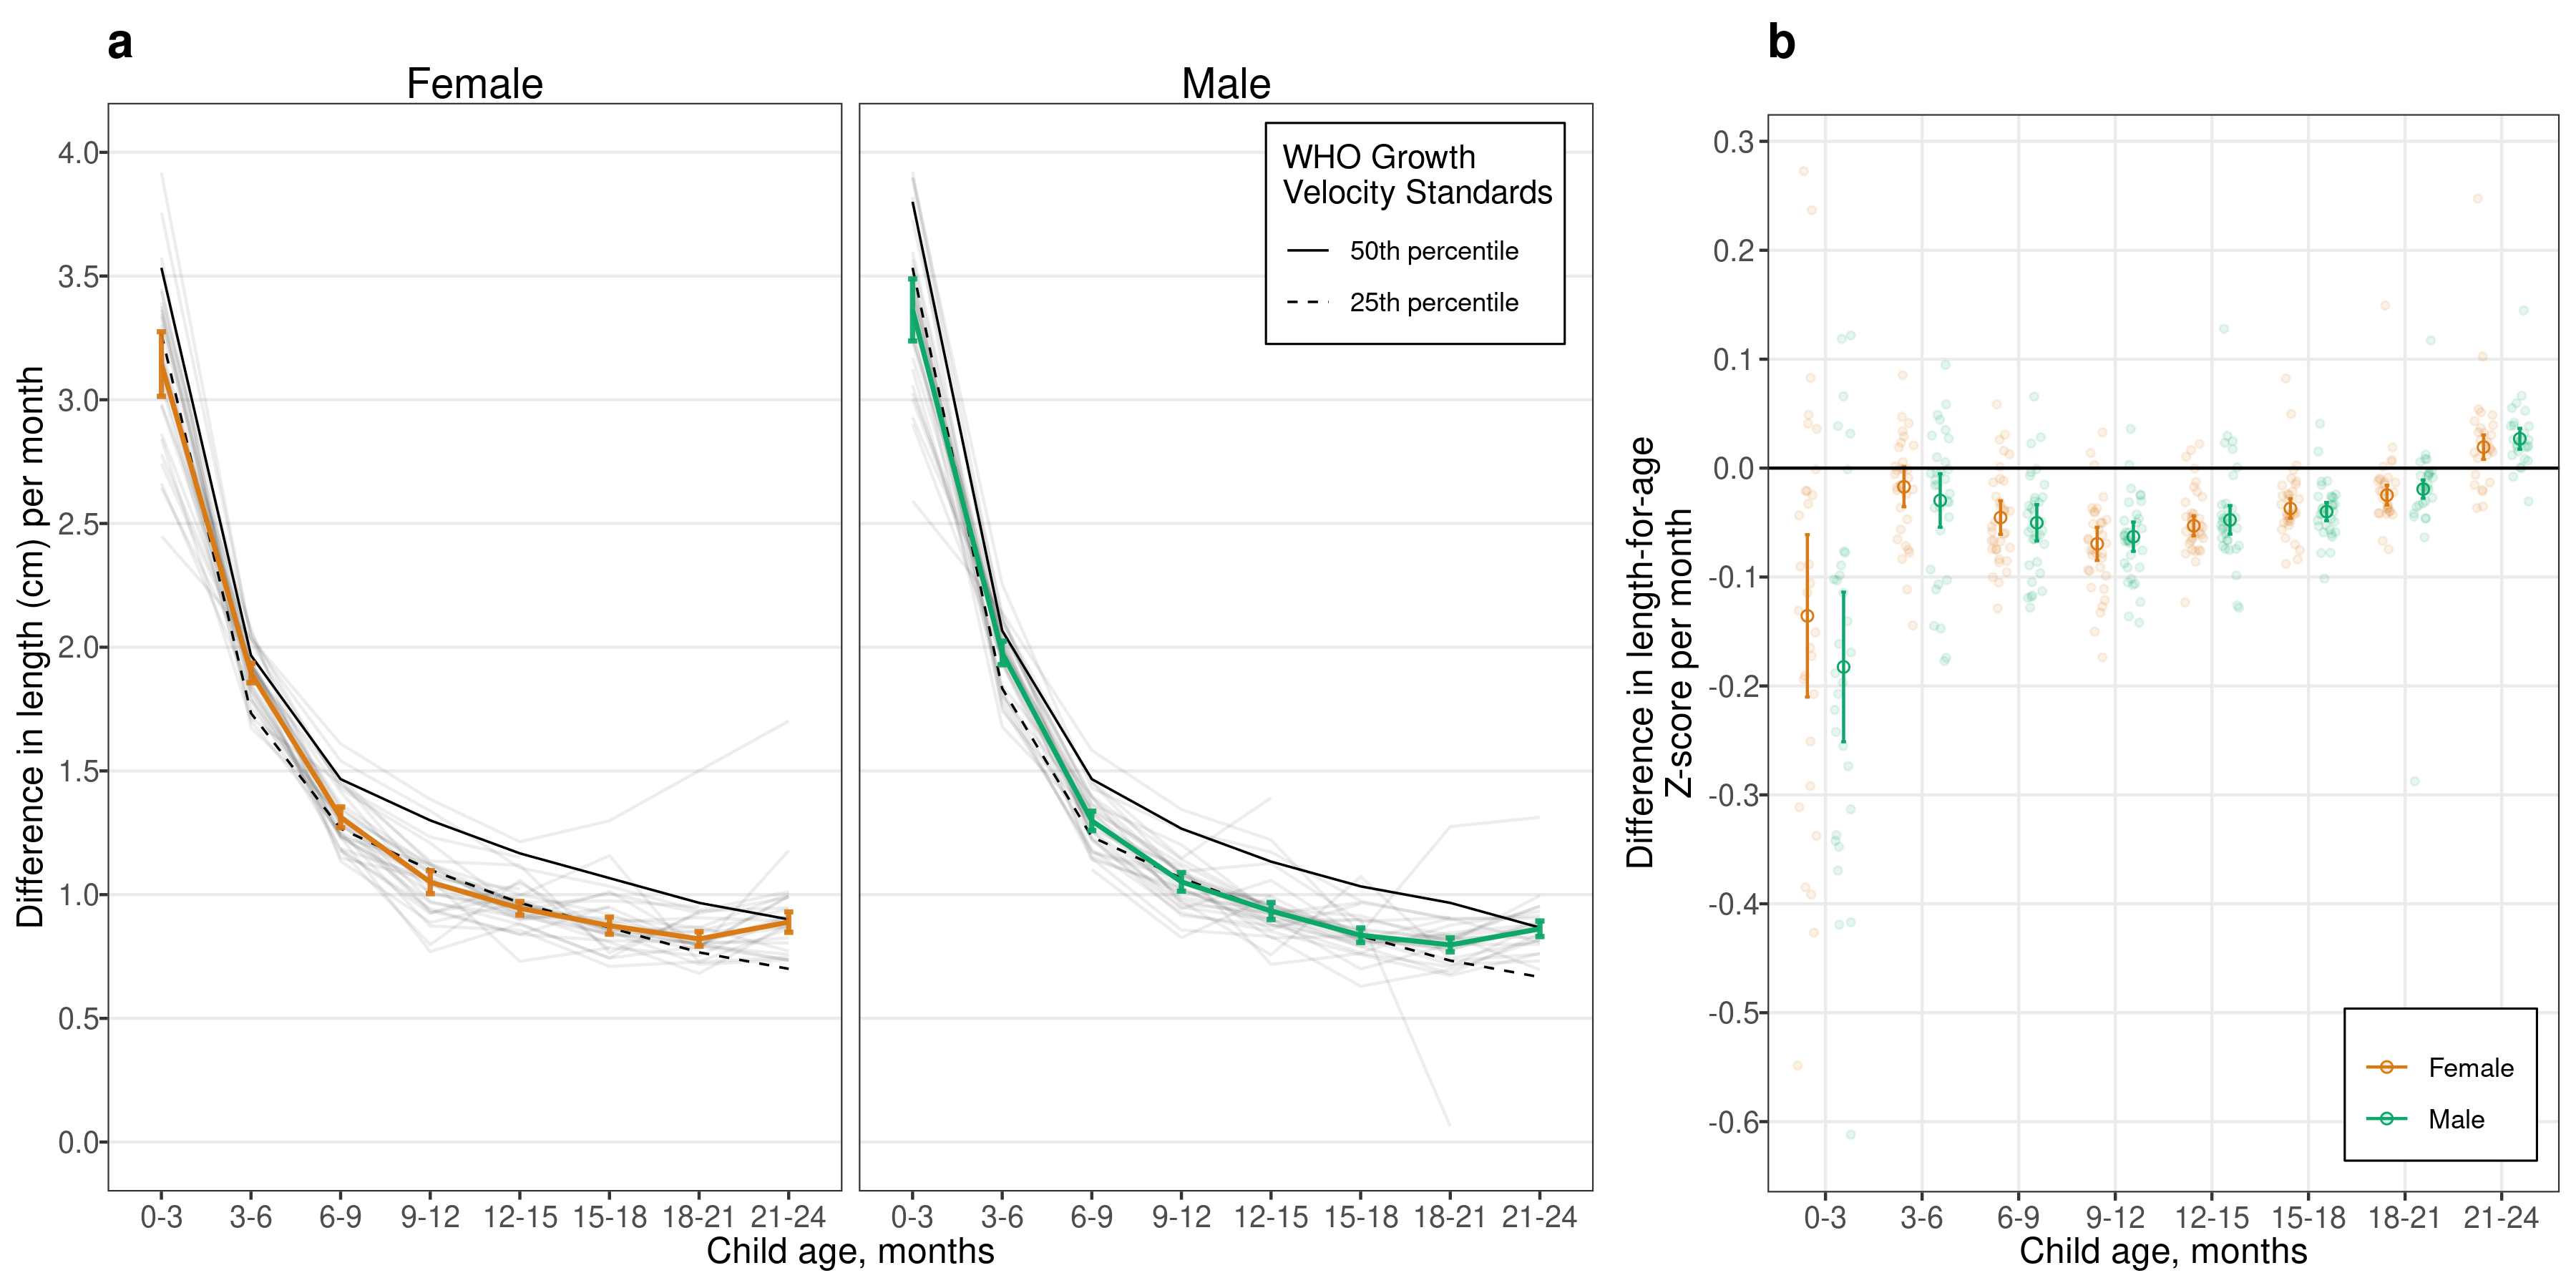
\includegraphics[width=50in]{figures//stunting/fig-stunt-2-vel-overall--allage-primary}

  \bibliography{book.bib,packages.bib}

\end{document}
